\pdfoutput=1
%%%%%%%% TEMPLATE FOR LATEX %%%%%%%%%%%%%%%%%

\documentclass{article}



\newenvironment{largetable}[1][htb]{
    \begin{sidewaystable}[#1]
}{
    \end{sidewaystable}
}

% \newenvironment{largetable}[1][htb]{
%     \begin{landscape}
%     \begin{table}[#1]
% }{
%     \end{table}
%     \end{landscape}
% }



% Recommended, but optional, packages for figures and better typesetting:
\usepackage{microtype}
\usepackage[dvipsnames,table,xcdraw]{xcolor}
\usepackage{graphicx}
\usepackage{afterpage}
\usepackage{caption}
\usepackage{subcaption}
\usepackage{float}
\usepackage{stfloats}
\usepackage{booktabs} % for professional tables
\usepackage{rotating}
\usepackage{tablefootnote}


% If your build breaks (sometimes temporarily if a hyperlink spans a page)
% please comment out the following usepackage line and replace
% \usepackage{template} with \usepackage[nohyperref]{template} above.
\usepackage{hyperref}


% Attempt to make hyperref and algorithmic work together better:
\newcommand{\theHalgorithm}{\arabic{algorithm}}

% For theorems and such
\usepackage{amsmath}
\usepackage{amssymb}
\usepackage{mathtools}
\usepackage{amsthm}

\usepackage[capitalize,noabbrev]{cleveref}



% Alter some LaTeX defaults for better treatment of figures:
% See p.105 of "TeX Unbound" for suggested values.
% See pp. 199-200 of Lamport's "LaTeX" book for details.
%   General parameters, for ALL pages:
\renewcommand{\topfraction}{0.9}	% max fraction of floats at top
\renewcommand{\bottomfraction}{0.9}	% max fraction of floats at bottom
%   Parameters for TEXT pages (not float pages):
\setcounter{topnumber}{5}
\setcounter{bottomnumber}{5}
\setcounter{totalnumber}{8}     % 2 may work better
\setcounter{dbltopnumber}{6}    % for 2-column pages
\renewcommand{\dbltopfraction}{0.9}	% fit big float above 2-col. text
\renewcommand{\textfraction}{0.07}	% allow minimal text w. figs
%   Parameters for FLOAT pages (not text pages):
\renewcommand{\floatpagefraction}{0.7}	% require fuller float pages
% N.B.: floatpagefraction MUST be less than topfraction !!
\renewcommand{\dblfloatpagefraction}{0.7}	% require fuller float pages

% remember to use [htp] or [htpb] for placement





%%%% OUR PACKAGES AND STUFF %%%%

\newcommand{\X}{\ensuremath{\mathbf{X}}\xspace}
\newcommand{\Y}{\ensuremath{\mathbf{Y}}\xspace}
\newcommand{\Gx}{\ensuremath{\mathbf{G}_X}\xspace}
\newcommand{\Gy}{\ensuremath{\mathbf{G}_Y}\xspace}
\newcommand{\Dx}{\ensuremath{\mathbf{D}_X}\xspace}
\newcommand{\Dy}{\ensuremath{\mathbf{D}_Y}\xspace}
\newcommand{\I}{\ensuremath{\mathbf{I}}\xspace}
\newcommand{\tr}{\ensuremath{\text{Tr}}\xspace}

\newcommand{\cA}{\mathcal{A}}
\newcommand{\cB}{\mathcal{B}}
\newcommand{\cC}{\mathcal{C}}
\newcommand{\cD}{\mathcal{D}}
\newcommand{\cE}{\mathcal{E}}
\newcommand{\cF}{\mathcal{F}}
\newcommand{\cG}{\mathcal{G}}
\newcommand{\cH}{\mathcal{H}}
\newcommand{\cI}{\mathcal{I}}
\newcommand{\cK}{\mathcal{K}}
\newcommand{\cL}{\mathcal{L}}
\newcommand{\cM}{\mathcal{M}}
\newcommand{\cN}{\mathcal{N}}
\newcommand{\cQ}{\mathcal{Q}}
\newcommand{\cS}{\mathcal{S}}
\newcommand{\cT}{\mathcal{T}}
\newcommand{\cX}{\mathcal{X}}
\newcommand{\cY}{\mathcal{Y}}
\newcommand{\cZ}{\mathcal{Z}}

\newcommand{\bA}{\mathbf{A}}
\newcommand{\bB}{\mathbf{B}}
\newcommand{\bC}{\mathbf{C}}
\newcommand{\bD}{\mathbf{D}}
\newcommand{\bE}{\mathbf{E}}
\newcommand{\bF}{\mathbf{F}}
\newcommand{\bG}{\mathbf{G}}
\newcommand{\bH}{\mathbf{H}}
\newcommand{\bI}{\mathbf{I}}
\newcommand{\bK}{\mathbf{K}}
\newcommand{\bL}{\mathbf{L}}
\newcommand{\bM}{\mathbf{M}}
\newcommand{\bN}{\mathbf{N}}
\newcommand{\bQ}{\mathbf{Q}}
\newcommand{\bS}{\mathbf{S}}
\newcommand{\bT}{\mathbf{T}}
\newcommand{\bX}{\mathbf{X}}
\newcommand{\bY}{\mathbf{Y}}
\newcommand{\bZ}{\mathbf{Z}}

\newcommand{\dist}{\text{Dist}}
\newcommand{\treedist}{\text{Dist}_T}
\newcommand{\dt}{d}
\newcommand{\children}{\text{children}\xspace}
\newcommand{\leaves}{\text{leaves}\xspace}
\newcommand{\lca}{\text{LCA}\xspace}
\newcommand{\cost}{\textup{Cost}}
\newcommand{\cd}{\textup{CostDecrease}}

\newcommand{\eps}{\varepsilon}

\DeclareMathOperator*{\argmax}{arg\,max}
\DeclareMathOperator*{\argmin}{arg\,min}


\newcommand{\abinline}[1]{\todo[inline, color=anna!30]{\textbf{AB:} #1}}


\usepackage[shortcuts]{extdash}
\usepackage{comment}
\usepackage{microtype}
\usepackage{amsthm}
\usepackage{multirow}
\usepackage{url}
\usepackage{tabularx}
\usepackage{booktabs}
\usepackage{bm}
\usepackage{extdash}
\usepackage{colortbl}
\usepackage{enumitem}

\usepackage{tikz}
\usepackage{pgfplots}
\pgfplotsset{compat=1.18}
\usepackage{circuitikz}
\usepackage{forest}
\usetikzlibrary{shapes}
\usetikzlibrary{positioning}
\usetikzlibrary{arrows}
\usetikzlibrary{decorations.pathmorphing}
\usetikzlibrary{math}
\usepackage{tikz-qtree}

\usepackage{svg}
% \usepackage{algorithm}
% \usepackage[algo2e,linesnumbered,ruled,vlined,noline,noend,nosemicolon]{algorithm2e}
% \usepackage[noend,algcompatible]{algpseudocode}
\usepackage{wrapfig}
\usepackage{pdflscape}
\usepackage{adjustbox}
\usepackage{nicematrix}
\usepackage{balance}


\newcommand*\circled[1]{\tikz[baseline=(char.base)]{
            \node[shape=circle,draw,inner sep=2pt] (char) {#1};}}
\newcommand*\putinsquare[1]{\tikz[baseline=(char.base)]{
            \node[shape=rectangle,draw,inner sep=2pt] (char) {#1};}}


\usepackage{amsmath}
\usepackage{thm-restate}
\usepackage{outlines}
\usepackage{natbib}




%symbols and abbreviations
\newcommand{\xx}{\colorbox{black}{\textcolor{red}{XX}}}



%%%%%%%%%%%%%%%%%%%%%%%%%%%%%%%%
% THEOREMS
%%%%%%%%%%%%%%%%%%%%%%%%%%%%%%%%
\theoremstyle{plain}
\newtheorem{theorem}{Theorem}[section]
\newtheorem{proposition}[theorem]{Proposition}
\newtheorem{lemma}[theorem]{Lemma}
\newtheorem{idea}[theorem]{Idea}
\newtheorem{fact}[theorem]{Fact}
\newtheorem{corollary}[theorem]{Corollary}
\theoremstyle{definition}
\newtheorem{definition}[theorem]{Definition}
\newtheorem{assumption}[theorem]{Assumption}
\theoremstyle{remark}
\newtheorem{remark}[theorem]{Remark}



%%%%%%%%%%%%%%%%%%%%%%%%%%%%%%%%
% Title and Authors
%%%%%%%%%%%%%%%%%%%%%%%%%%%%%%%%
% Use the following line for the initial blind version submitted for review:
% \usepackage{template2025}

% If accepted, instead use the following line for the camera-ready submission:
\usepackage[accepted]{template}


% Todonotes is useful during development; simply uncomment the next line
%    and comment out the line below the next line to turn off comments
\usepackage[disable,textsize=tiny]{todonotes}
% \usepackage[textsize=tiny]{todonotes}



% The \templatetitle you define below is probably too long as a header.
% Therefore, a short form for the running title is supplied here:
\templatetitlerunning{I Want 'Em All (At Once) -- Ultrametric Cluster Hierarchies}

\begin{document}

\twocolumn[
\templatetitle{I Want 'Em All (At Once) -- Ultrametric Cluster Hierarchies}

% Ultrametric Cluster Hierarchies Beyond HDBSCAN

% It is OKAY to include author information, even for blind
% submissions: the style file will automatically remove it for you
% unless you've provided the [accepted] option to the template2024
% package.

% List of affiliations: The first argument should be a (short)
% identifier you will use later to specify author affiliations
% Academic affiliations should list Department, University, City, Region, Country
% Industry affiliations should list Company, City, Region, Country

% You can specify symbols, otherwise they are numbered in order.
% Ideally, you should not use this facility. Affiliations will be numbered
% in order of appearance and this is the preferred way.
\templatesetsymbol{equal}{*}

\begin{templateauthorlist}


\templateauthor{Andrew Draganov}{equal,aarhus}
\templateauthor{Pascal Weber}{equal,vienna,docschool,ds}
\templateauthor{Rasmus Skibdahl Melanchton Jørgensen}{aarhus}
\templateauthor{Anna Beer}{vienna}
\templateauthor{Claudia Plant}{vienna,ds}
\templateauthor{Ira Assent}{aarhus}
\end{templateauthorlist}

\templateaffiliation{aarhus}{\href{https://cs.au.dk/research/data-intensive-systems}{Department of Computer Science, Aarhus University}, Aarhus, Denmark}
\templateaffiliation{vienna}{\href{https://dm.cs.univie.ac.at/}{Data Mining and Machine Learning, University of Vienna}, Vienna, Austria}
\templateaffiliation{docschool}{\href{https://docs.univie.ac.at/}{UniVie Doctoral School Computer Science, University of Vienna}, Vienna, Austria}
\templateaffiliation{ds}{\href{https://datascience.univie.ac.at/}{Data Science @ Uni Vienna, University of Vienna}, Vienna, Austria}


\templatecorrespondingauthor{Andrew Draganov}{\href{mailto:draganovandrew@cs.au.dk?subject=[SHIP]\%20I\%20want\%20to\%20reach\%20out\&cc=mailto:pascal.weber@univie.ac.at}{draganovandrew@cs.au.dk}}
\templatecorrespondingauthor{Pascal Weber}{\href{mailto:pascal.weber@univie.ac.at?subject=[SHIP]\%20I\%20want\%20to\%20reach\%20out\&cc=draganovandrew@cs.au.dk}{pascal.weber@univie.ac.at}}

% You may provide any keywords that you
% find helpful for describing your paper; these are used to populate
% the "keywords" metadata in the PDF but will not be shown in the document
\templatekeywords{clustering, hierarchies, efficiency, ultrametrics}

\vskip 0.3in
]

% this must go after the closing bracket ] following \twocolumn[ ...

% This command actually creates the footnote in the first column
% listing the affiliations and the copyright notice.
% The command takes one argument, which is text to display at the start of the footnote.
% The \templateEqualContribution command is standard text for equal contribution.
% Remove it (just {}) if you do not need this facility.

%\printAffiliationsAndNotice{}  % leave blank if no need to mention equal contribution
\printAffiliationsAndNotice{\templateEqualContribution} % otherwise use the standard text.

\begin{abstract}

Hierarchical clustering is a powerful tool for exploratory data analysis, organizing data into a tree of clusterings from which a partition can be chosen. This paper generalizes these ideas by proving that, for any reasonable hierarchy, one can optimally solve any center-based clustering objective over it (such as $k$-means). Moreover, these solutions can be found exceedingly quickly and are \emph{themselves} necessarily hierarchical. 
%Thus, given a cluster tree, we show that one can quickly generate a myriad of \emph{new} hierarchies from it. 
Thus, given a cluster tree, we show that one can quickly access a plethora of new, equally meaningful hierarchies.
Just as in standard hierarchical clustering, one can then choose any desired partition from these new hierarchies. We conclude by verifying the utility of our proposed techniques across datasets, hierarchies, and partitioning schemes.


\end{abstract}

\section{Introduction}

% Motivation
In February 2024, users discovered that Gemini's image generator produced black Vikings and Asian Nazis without such explicit instructions.
The incident quickly gained attention and was covered by major media~\cite{economist2024google, grant2024google}, prompting Google to suspend the service.
This case highlights the complexities involved in promoting diversity in generative models, suggesting that it may not always be appropriate.
Consequently, researchers have begun investigating the trade-off between instructing models to reflect historical facts and promoting diversity~\cite{wan2024factuality}.
Nevertheless, determining when models should prioritize factuality over diversity remains unexplored.

\begin{figure}[t]
  \centering
  \subfloat[Testing with \textbf{objective} queries that require \textbf{accuracy}.]{
    \includegraphics[width=1.0\linewidth]{Figures/obj-cover.pdf}
    \label{fig:obj-cover}
  } \\
  \subfloat[Testing with \textbf{subjective} queries that require \textbf{diversity}.]{
    \includegraphics[width=1.0\linewidth]{Figures/subj-cover.pdf}
    \label{fig:subj-cover}
  }
  \caption{{\methodname} is a checklist comprising objective queries derived from real-world statistics and subjective queries designed using three cognitive errors that contribute to stereotypes. It includes queries designed for LLMs and T2I models.}
\end{figure}

% Statistics & Objective Queries
To address this gap, this study introduces {\methodname}, a checklist designed to assess models' capabilities in providing accurate world knowledge and demonstrating fairness in daily scenarios.
For world knowledge assessment, we collect 19 key statistics on U.S. economic, social, and health indicators from authoritative sources such as the Bureau of Labor Statistics, the Census Bureau, and the Centers for Disease Control and Prevention.
Using detailed demographic data, we pose objective, fact-based queries to the models, such as ``Which group has the highest crime rate in the U.S.?''—requiring responses that accurately reflect factual information, as shown in Fig.~\ref{fig:obj-cover}.
Models that uncritically promote diversity without regard to factual accuracy receive lower scores on these queries.

% Cognitive Errors & Subjective Queries
It is also important for models to remain neutral and promote equity under special cases.
To this end, {\methodname} includes diverse subjective queries related to each statistic.
Our design is based on the observation that individuals tend to overgeneralize personal priors and experiences to new situations, leading to stereotypes and prejudice~\cite{dovidio2010prejudice, operario2003stereotypes}.
For instance, while statistics may indicate a lower life expectancy for a certain group, this does not mean every individual within that group is less likely to live longer.
Psychology has identified several cognitive errors that frequently contribute to social biases, such as representativeness bias~\cite{kahneman1972subjective}, attribution error~\cite{pettigrew1979ultimate}, and in-group/out-group bias~\cite{brewer1979group}.
Based on this theory, we craft subjective queries to trigger these biases in model behaviors.
Fig.~\ref{fig:subj-cover} shows two examples on AI models.

% Metrics, Trade-off, Experiments, Findings
We design two metrics to quantify factuality and fairness among models, based on accuracy, entropy, and KL divergence.
Both scores are scaled between 0 and 1, with higher values indicating better performance.
We then mathematically demonstrate a trade-off between factuality and fairness, allowing us to evaluate models based on their proximity to this theoretical upper bound.
Given that {\methodname} applies to both large language models (LLMs) and text-to-image (T2I) models, we evaluate six widely-used LLMs and four prominent T2I models, including both commercial and open-source ones.
Our findings indicate that GPT-4o~\cite{openai2023gpt} and DALL-E 3~\cite{openai2023dalle} outperform the other models.
Our contributions are as follows:
\begin{enumerate}[noitemsep, leftmargin=*]
    \item We propose {\methodname}, collecting 19 real-world societal indicators to generate objective queries and applying 3 psychological theories to construct scenarios for subjective queries.
    \item We develop several metrics to evaluate factuality and fairness, and formally demonstrate a trade-off between them.
    \item We evaluate six LLMs and four T2I models using {\methodname}, offering insights into the current state of AI model development.
\end{enumerate}
\section{Ultrametrics and Tree Representations}
\label{sec:ultrametrics}

We begin by formally introducing the data structure representing ultrametric spaces as it facilitates solving center-based clustering tasks quickly. The upcoming results operate over a generalization of the standard ultrametric:
\begin{restatable}{definition}{RelaxedUltrametric}
    \label{def:relaxed_ultrametric}
    Let $L$ be a set. Then $d: L \times L \rightarrow \mathbb{R}_{\geq 0}$ is a \emph{relaxed ultrametric} over $L$ if, for all $\ell_i, \ell_j, \ell_k \in L$, the
    following conditions are satisfied:
    \begin{align*}
        d(\ell_i, \ell_j) &= d(\ell_j, \ell_i) \geq 0 \\
        d(\ell_i, \ell_k) &\leq \max( d(\ell_i, \ell_j), d(\ell_j, \ell_k)).
    \end{align*}
\end{restatable}
Note that the standard ultrametric is a restriction that additionally requires $\dt(\ell_i, \ell_i) = 0$. Thus, not all relaxed ultrametrics are distances as $\dt(\ell_i, \ell_i) \gneq 0$ is allowed. Still, we use the word ``distance'' for readability.
%
We represent relaxed ultrametric relationships via the following data structure:

\begin{definition}
    \label{def:lca_tree}
    A \emph{lowest-common-ancestor tree} (\emph{LCA-tree}) is a rooted tree $T$ such that every node $\eta \in T$ has value $d(\eta) \geq 0$ associated with it. We write $\eta_i \preceq \eta_j$ to indicate that $\eta_j$ lies on the path from $\eta_i$ to the root and $\eta_i \lor \eta_j$ to refer to the LCA of $\eta_i$ and $\eta_j$. We say that the \emph{LCA-distance} between two leaves $\ell_i, \ell_j \in T$ is given by $d(\ell_i \lor \ell_j)$.
\end{definition}

An LCA-tree is not necessarily binary: if three or more subtrees are all equidistant, they can all be children of the same node. While similar data structures already exist for standard ultrametrics \citep{ultrametric_lca_def, memory_efficient_minimax}, the following theorem (proof in \ref{app:ultrametric_proofs}) states that it can also encode all relaxed ultrametrics:\footnote{
Note that \textit{relaxed} ultrametrics cannot be represented via shortest-path distances through a tree as is commonly done for ultrametrics \citep{ultrametrics_root_equidist} as $d(\ell_i, \ell_i) > 0$ is possible.}


\begin{restatable}{theorem}{UltrametricEquivalency}
    \label{thm:ultrametric_equivalency}
    Let $(L, d')$ be a finite relaxed ultrametric space. Then there exists LCA-tree $T$ with LCA-distance $d$ and a bijection $f:L \leftrightarrow \text{leaves}(T)$ such that, for all $\ell_i, \ell_j \in L$, $d'(\ell_i, \ell_j) = d \left( f(\ell_i) \lor f(\ell_j) \right)$.
\end{restatable}

This is visualized by the first box of Figure \ref{fig:overview}. It shows a minimum spanning tree (MST) over some data on the left. In this MST, the minimax ultrametric is given by the weight of the largest edge in the path between two nodes \cite{minimax_distance}. For example, the minimax distance between nodes $\circled{1}$ and $\circled{4}$ is $\putinsquare{5}$. The right-hand side of the first box of Figure 1 then stores these minimax distances in an LCA-tree where the LCA of nodes $\circled{1}$ and $\circled{4}$ has value $5$.

We show in Appendix \ref{app:ultrametric_proofs} that all LCA-trees are relaxed ultrametrics as long as they satisfy the following conditions:

\begin{restatable}{corollary}{LCAcorollary}
    \label{cor:ultrametric_lca}
    Let $T$ be an LCA-tree. For any leaf $\ell \in T$, let $p(\ell) = [\ell, \eta_a, \ldots, \eta_b, r(T)]$ be the path from $\ell$ to the root of the tree $r(T)$.
    Then the LCA-distances on $T$ form a relaxed ultrametric if and only if, for all $\ell \in \text{leaves}(T)$ and $\eta_i, \eta_j \in p(\ell)$, the following conditions are satisfied:
    \[\text{\emph{(1)}} \quad d(\ell) \geq 0 \quad \text{and} \quad \text{\emph{(2)}} \quad \eta_i \preceq \eta_j \implies d(\eta_i) \leq d(\eta_j).\]
\end{restatable}
%
Corollary \ref{cor:ultrametric_lca} describes a key property: if a tree's node values grow along paths from the leaves to the root, then the corresponding LCA-distances are a relaxed ultrametric. This is the natural representation of a hierarchy: since the subtrees grow in size as we go towards the root, the values corresponding to those subtrees also grow. Thus, relaxed ultrametrics and hierarchies are equivalent notions. Going forward, we assume that a relaxed ultrametric is given in its LCA-tree form, satisfying the properties in Corollary \ref{cor:ultrametric_lca}.
\section{Center-based clustering in ultrametrics}
\label{sec:clustering_theory}
%
Our primary theoretical result is that the $k$-means, $k$-median, and $k$-center objectives can be solved optimally in a relaxed ultrametric. Furthermore, these solutions are hierarchical and can all be found in $\texttt{Sort}(n)$ time.\footnote{ I.e., the time required to sort $O(n)$ distances in the metric. Although sorting is thought of as requiring $O(n \log n)$ time, in many settings, it only requires $O(n \log \log n)$ time \citep{sort_time}.}
%
\paragraph{Notation.} We define the \emph{$(k, z)$-clustering} and the \emph{$k$-center clustering} objectives over $T$ as finding the set of centers $\mathbf{C} \subseteq \text{leaves}(T)$ with $|\bC| = k$ which minimize, respectively, 
\[\cost_z(T, \bC) = \underbrace{ \sum_{\ell \in \text{leaves}(T)} \min_{c \in \bC} \dt(\ell, c)^z}_{(k, z)\text{-clustering objective}},\]
%
\[\cost_\infty(T, \bC) = \underbrace{\max_{\ell \in \text{leaves}(T)} \min_{c \in \bC} \dt(\ell, c)}_{k\text{-center clustering objective}}.\]
%
Note that the $(k, z)$-clustering task gives us the well-known $k$-median and $k$-means tasks for $z=1$ and $z=2$. Let us now define what it means for a clustering to be hierarchical. Given a set of points $L$, we define a \emph{cluster} $C$ as any subset of $L$. We then define a \emph{partition} $\mathcal{P}_k = \{C_1, \ldots, C_k\}$ as any \emph{non-overlapping} set of $k$ clusters, i.e., for all $C_i, C_j \in \mathcal{P}$, $C_i \cap C_j = \emptyset$. We now define cluster hierarchies:%This brings us to the following definition for cluster hierarchies (visualized in box 2 of \Cref{fig:overview}):


\begin{restatable}{definition}{Hierarchy}[\citet{hierarchical_center_based}]
    \label{def:hierarchical_clusters}
     A \emph{cluster hierarchy} $\mathcal{H} = \{\mathcal{P}_1, \ldots, \mathcal{P}_n\}$ is a set of partitions with
    \begin{enumerate}[topsep=0pt,itemsep=0ex,partopsep=0ex,parsep=1ex]
        \item for $k=1$, $\mathcal{P}_1 \subseteq L$, and
        \item for $1 < k \leq n$, $\mathcal{P}_k = \left( \mathcal{P}_{k-1} \symbol{92} C_i \right) \cup \{C_j, C_l\}$, such that $C_i = C_j \cup C_l \in \mathcal{P}_{k-1}$ with $C_j \cap C_l = \emptyset$ and $i \neq j \neq l$.
    \end{enumerate}
    We say a cluster $C_i \in \mathcal{H}$ if $\exists \; \mathcal{P}_j \in \mathcal{H}$ with $C_i \in \mathcal{P}_j$.
    %We write $\mathcal{H}[C_i]$ to denote the cluster hierarchy rooted at cluster $C_i$.
    %We say $\mathcal{P}'$ \textbf{indirectly} belongs to $\mathcal{H}$ if $\mathcal{P}' \subset \bigcup_{\mathcal{P}_i \in \mathcal{H}} \mathcal{P}_i$.
\end{restatable}
\noindent This means that the partition $\mathcal{P}_k$ is obtained by splitting a cluster from $\mathcal{P}_{k-1}$ in two. 
Thus, all cluster hierarchies can be represented as a rooted tree. We depict this in \cref{fig:overview} (middle), where the hierarchy is obtained by subdividing the clusters. We can now state our primary theoretical result:
%
\begin{restatable}{theorem}{maintheorem}
    \label{thm:optimal_clusters}
    Let $(L, d)$ be a finite relaxed ultrametric space represented over an LCA-tree $T$. Let $n = |L|$ and $z \in \mathbb{Z}_{>0}$.
    Then, for both the $k$-center and $(k, z)$-clustering objectives on $T$, there exists an algorithm which finds the optimal solutions $\{\mathbf{C}_1, \ldots, \mathbf{C}_n\}$ for all $k \in \mathbb{N}_n$ in $\texttt{Sort}(n)$ time. Furthermore, the respective partitions $\mathcal{H} = \{\mathcal{P}_1, \ldots, \mathcal{P}_n\}$ obtained by assigning all leaves in $T$ to their closest center satisfy Definition \ref{def:hierarchical_clusters}.
\end{restatable}
%
Theorem \ref{thm:optimal_clusters} states that given any LCA-tree over a relaxed ultrametric, it takes $\texttt{Sort}(n)$ time to find the optimal solutions for $k$-means, $k$-median or $k$-center across all values of $k$ and that these solutions are hierarchical. While subsets of this are known for specific ultrametrics \cite{hierarchical_kmedian, beer2023connecting}, our runtime improves over the previous state of the art, and we are not aware of a comprehensive treatment of this subject over all ultrametrics and center-based clustering objectives.
%For example, \cite{beer2023connecting} showed that one can optimally solve $k$-center given the minimax distances in $O(n^2)$ time. Similarly, \cite{hierarchical_kmedian} showed that $k$-median can be solved optimally in $O(n\log^2(n^2 + \Delta^2))$ time given a hierarchically well-separated tree (HST).\footnote{Here, $\log \Delta$ is the depth of the HST.} Nonetheless, our runtime improves over those listed above, and we are not aware of a comprehensive treatment of this subject over all ultrametrics and center-based clustering objectives. 
%
\paragraph{Proof Overview.} The $k$-center part of this result is an extension of the farthest-first traversal algorithm where one picks each subsequent center as the point that is farthest from the current set of centers \citep{farthest_first, Har-Peled}. In essence, Appendix \ref{app:k_center_proof} shows that the farthest-first traversal algorithm becomes optimal under the strong triangle inequality. Then, we show in Appendix \ref{app:k_z_clustering_proof} that the $(k, z)$-clustering objectives in a relaxed ultrametric can be reduced to the $k$-center one. Specifically, given an LCA-tree $T$ on which to do $(k, z)$-clustering, there exists a \emph{new} LCA-tree $T'$ such that an optimal $k$-center solution on $T'$ \emph{is} the optimal $(k, z)$-clustering solution on $T$. Interestingly, even if this reduction is applied in a standard ultrametric, it requires the definition of relaxed ultrametrics to go through.
Finally, the runtime bottleneck for $k$-center lies in sorting the $O(n)$ unique distances in the ultrametric so that we may apply farthest-first traversal. The reduction from $(k, z)$-clustering only requires $O(n)$ time. Thus, the bottleneck remains unchanged for $(k, z)$-clustering. We verify by a worst-case example that our runtime is tight: one cannot find the optimal centers for all values of $k \in \mathbb{N}_n$ faster than in $\texttt{Sort}(n)$ time (Lemma \ref{lma:worst_case}).

\paragraph{Takeaway.} An interesting consequence of Corollary \ref{cor:ultrametric_lca} and Theorem \ref{thm:optimal_clusters} is that these center-based cluster hierarchies \emph{themselves} constitute relaxed ultrametrics. That is, let $\mathcal{H}$ be a hierarchy of optimal $k$-center or $(k, z)$-clustering solutions from Theorem \ref{thm:optimal_clusters}. For each cluster $C$ in this hierarchy, consider the cost $d_{cost}(C)$ of assigning all of its points to a single optimal center. As we traverse the tree towards the root, these costs will necessarily grow (see Lemma \ref{lma:optimal_subtrees} in Appendix \ref{app:k_z_clustering_proof}). Thus, by Corollary \ref{cor:ultrametric_lca}, the hierarchy $\mathcal{H}$ with LCA-distances $d_{cost}$ \emph{must} be a relaxed ultrametric. This is precisely what facilitates our reduction from the $(k, z)$-clustering setting to the $k$-center one. Indeed, any LCA-tree satisfying the properties in Corollary \ref{cor:ultrametric_lca} \emph{is} its own optimal $k$-center hierarchy (non-binary LCA-trees can be binarized while preserving the LCA-distances to recover the equivalence to the $k$-center hierarchy).

\section{Choosing a Partition}\label{sec:best_clustering}

Theorem \ref{thm:optimal_clusters} gives us the optimal center-based clustering solutions for all values of $k$ at once. If we simply require the solution for a specific $k$ then this is sufficient. However, what if we are instead interested in the ``best'' clustering from this hierarchy? To this end, this section discusses how known techniques for obtaining a partition can be applied to Section \ref{sec:clustering_theory}'s hierarchies in $O(n)$ time.

\subsection{Cluster Selection Criteria}

\subsubsection{Feasibility of the Elbow Method}\label{sec:elbow}

One of the most common methods for choosing a ``best'' clustering is the elbow method \citep{elbow_original}. Here, one is given a set of values of $k$, $[k_1, k_2, \ldots, k_f]$, and a set of corresponding partitions $\mathcal{P} = [\mathcal{P}_{1}, \mathcal{P}_{2}, \ldots, \mathcal{P}_{f}]$. Each partition incurs a cost $\mathcal{L} = [\mathcal{L}_{1}, \mathcal{L}_{2}, \ldots, \mathcal{L}_{f}]$ with respect to the clustering objective, where $\mathcal{L}_i = \sum_{C \in \mathcal{P}_i} \mathcal{L}(C)$. This gives us a plot of costs over the different values of $k$. Informally, the \emph{elbow method} chooses the partition $\mathcal{P}_i$ whose cost $\mathcal{L}_i$ looks to be at a sharp point in this curve.

Due to the NP-hardness of $k$-means clustering \cite{kmeans_hardness_1}, standard elbow plots can only compute approximate solutions, traditionally done sequentially for each $k$ \cite{elbow_issues}. However, the elbow method is surprisingly viable in the ultrametric setting: Theorem \ref{thm:optimal_clusters} yields optimal clusterings for all $k$ values at once, eliminating both computational overhead and approximation errors. Moreover, we show that the relaxed ultrametric's elbow plot for $(k, z)$-clustering is guaranteed to be convex:

\begin{restatable}{corollary}{ElbowPlotCor}
    \label{cor:elbow_plot}
    Let $\mathcal{P}$ and $\mathcal{L}$ correspond to the $n$ partitions and losses obtained in accordance with Theorem \ref{thm:optimal_clusters} for the $(k, z$)-clustering objective. Let $\Delta_i = \mathcal{L}_{i+1} - \mathcal{L}_i$. Then either $\Delta_{i} < \Delta_{i+1} \leq 0$ or $\Delta_{i} = \Delta_{i+1} = 0$ for all $i \in [n-1]$.
\end{restatable}

The idea here is that $\Delta_i$ represents the elbow plot's first derivative at $k=i$. Thus, Corollary \ref{cor:elbow_plot} states that the elbow plot's slope is steepest at $k=1$ and monotonically levels out to 0 as $k \rightarrow n$. We prove this in Appendix \ref{app:ultrametric_elbow}, where we also specify how we determine the index of the elbow. We depict relaxed ultrametric elbow plots in the $(k, z)$-clustering setting for various values of $z$ in Figure \ref{fig:elbow_plot}, where we see that the plots are indeed convex.

\begin{figure}[t]
    \centering
    \vspace{0.2em}
    \resizebox{0.98\linewidth}{!}{%
    \begin{tikzpicture}
        \node[inner sep=0pt] (zoomed_out) at (0, 0) {\includegraphics[width=\linewidth, trim={0.75cm, 0.50cm, 0.5cm, 0.3cm}, clip]{figures/elbow_plot_large.pdf}};

        % Draw Zoomed in Figure
        \node[inner sep=0pt] (zoomed_in) at (0.75, 0.75){\includegraphics[width=0.72\linewidth, trim={1.1cm, 0.7cm, 0.5cm, 0.3cm}, clip]{figures/elbow_plot_zoomed_in.pdf}};
        \draw[red, thick, opacity=0.55] ($(zoomed_in.north west)$) rectangle ($(zoomed_in.south east)$);

        % Draw Zoom Box
        \draw[red, very thick, dotted, opacity=0.8] (-3.72,-2.9) rectangle (-1,-2.2);
    
        % Draw connecting lines from rectangle corners to zoomed image
        \draw[red, very thick, dashed, opacity=0.6] (-3.72,-2.2) -- (-2.25,2.99);
        \draw[red, very thick, dashed, opacity=0.6] (-1,-2.9) -- (3.72,-1.485);

        \node[inner sep=0pt] (a) at (-1.52, -1.67) {\tiny \textcolor{gray}{6}};
        \node[inner sep=0pt] (a) at (-1.31, -1.67) {\tiny \textcolor{gray}{7}};
        \node[inner sep=0pt] (a) at (-0.05, -1.67) {\tiny \textcolor{gray}{14}};

        \fill[white] (2.43,-1.84) rectangle (2.68,-1.6);
        \node[inner sep=0pt] (a) at (2.55, -1.67) {\tiny \textcolor{gray}{28}};

        \fill[white] (2.98,-1.82) rectangle (3.22,-1.6);
        \node[inner sep=0pt] (a) at (3.1, -1.67) {\tiny \textcolor{gray}{31}};

        \node[inner sep=0pt] (a) at (-3.76, -3.27) {\small \textcolor{darkgray}{0}};
        \node[inner sep=0pt] (a) at (-0.65, -3.27) {\textcolor{darkgray}{40}};
        \node[inner sep=0pt] (a) at (2.475, -3.27) {\textcolor{darkgray}{80}};
        \node[inner sep=0pt] (a) at (4.05, -3.27) {\textcolor{black}{\dots}};
        \node[inner sep=0pt] (a) at (0, -3.7) {\textcolor{darkgray}{Number of clusters ($k$)}};

        \node[inner sep=0pt] (a) at (-4.3, -2.75) {\small \textcolor{darkgray}{0}};
        \node[inner sep=0pt] (a) at (-4.3, 2.95) {\textcolor{darkgray}{1}};
        \node[inner sep=0pt] (a) at (-4.5, 0) {\textcolor{darkgray}{\rotatebox{90}{Normalized cost}}};        
    \end{tikzpicture}%
    }
    \vspace*{-0.4em}
    \caption{Example elbow plots for the $z=1, 2, 3, 4\text{, and }5$ settings under the dc-dist ultrametric on the D31 synthetic dataset. Elbow locations (circles) are determined using all $k$ from $1$ to $n$.}
    \label{fig:elbow_plot}
% \end{wrapfigure}
\end{figure}


\subsubsection{Thresholding the Tree}

While Corollary \ref{cor:elbow_plot} shows that the elbow method is reasonable in the ultrametric setting, it still has two main drawbacks. \emph{First}, the choice of the elbow is arbitrary, and it is unclear whether the best technique exists \citep{elbow_issues}. \emph{Second}, the elbow method is restricted to a single partition for each value of $k$. Although the cluster hierarchy can be cut in many ways to obtain $k$ clusters, the elbow method can only produce one of these partitions for any value of $k$.

One alternative is to threshold the cluster hierarchy, as done in single-linkage clustering or DBSCAN (see \citet{hdbscan}). Specifically, let $\varepsilon$ be any user-defined threshold parameter. We now (1) label the nodes of our cluster hierarchy by their costs as discussed at the end of Section \ref{sec:clustering_theory} and (2) report all clusters whose cost is less than $\varepsilon$, both in $O(n)$ time.
We further discuss this in \Cref{app:thresholding}.


\subsubsection{Cluster Value Functions} \label{sec:clustervaluefunction}

Rather than picking clusters based on their costs, one can also assign a \emph{new} value function to clusters and choose the partition that maximizes the sum of these values. Importantly, such a partition may not be attainable by choosing a value of $k$ or thresholding the clusters' costs in the hierarchy. For example, HDBSCAN uses the \emph{stability} objective to choose the clusters from a hierarchy that persist for the largest range of threshold values. Given any cluster hierarchy obtained via Theorem \ref{thm:optimal_clusters} and any reasonable value function, one can find the partition that maximizes this value function in $O(n)$ time. We detail this in Appendix \ref{app:cluster_merging_rules}. 


\subsection{Generalizing to Noisy Settings}

For a given LCA-tree $T$ and any node $\eta \in T$, one can remove the subtree rooted at $\eta$ from $T$ without affecting Corollary \ref{cor:ultrametric_lca}.
This allows handling additional noise points consistently, e.g., \citet{k-center-q-coverage, hdbscan}.

% To be consistent with the literature treating additional noise points in the data \citep{k-center-q-coverage, hdbscan}, we point out that one can prune nodes away from an LCA-tree without compromising our theoretical results. 
% Namely, given an LCA-tree $T$ and any node $\eta \in T$, one can remove the subtree rooted at $\eta$ from $T$ without affecting Corollary \ref{cor:ultrametric_lca}. Thus, pruning away subtrees does not affect any of the tree's ultrametric properties.

For example, consider a minimum-cluster-size parameter $\mu \in \mathbb{Z}_{+}$ and a cluster hierarchy $\mathcal{H}$ obtained via Theorem \ref{thm:optimal_clusters}. Then, for some cluster $C_i$ with $|C_i| < \mu$, we can prune the hierarchy by removing the cluster trees rooted at $C_i$ in $O(n)$ time \citep{hdbscan}. We can, therefore, obtain any desired clustering over this pruned hierarchy, guaranteeing that every cluster in the returned partition will have a size greater than or equal to the minimum cluster size. 


\subsection{Integrating Multiple Partition Methods} \label{sec:integrating_multiple_partition_methods}

Lastly, we note that we can combine results of several partitions without notable impact on runtime. As Section \ref{sec:experiments} confirms, fitting an ultrametric essentially always requires longer than $O(n \log n)$ time. Given such an ultrametric, we can find hierarchies of optimal center-based clustering solutions in $\texttt{Sort}(n) \leq O(n \log n)$ time (Section \ref{sec:clustering_theory}). Furthermore, we presented several $O(n) < \texttt{Sort}(n)$-time methods for choosing a partition. As Figure \ref{fig:runtime_barplot} highlights, the time it takes to fit the density-connectivity ultrametric dwarfs the time for finding a hierarchy or partition.
%
\begin{figure}
    \centering
    \vspace*{0.2em}
    \resizebox{\linewidth}{!}{
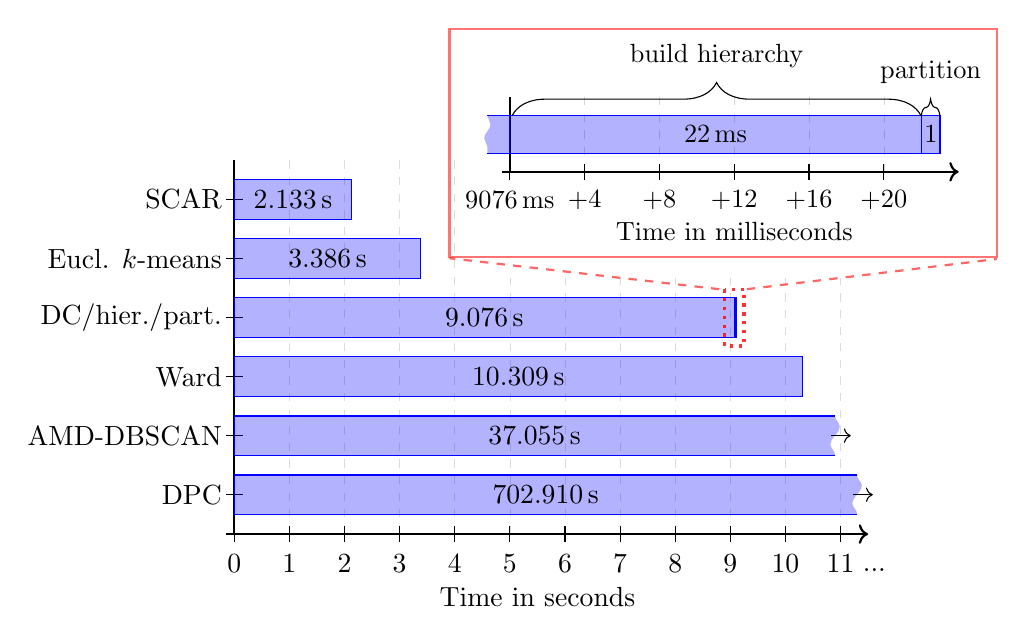
\begin{tikzpicture}[inner sep=0]

% Cover tree      00:00.322  
% DC tree         00:09.076  
% k-means         00:00.022  
% Stability       00:00.002  
% MoE             00:00.001  
% Elbow           00:00.001  
% Eucl. k-means   00:03.386  
% Eucl. k-means’  00:03.521  
% Ward            00:10.309  
% OPTICS          00:33.109  
% DPC             11:42.910   702.910
% SCAR            00:02.133  

\tikzmath{
	\ymax = 4.75;
	\ydc = 2.75;
	\dcTime = 9.076; \hierTime = 0.022; \partTime = 0.001;
	\dcTotalTime = {floor((\dcTime + \hierTime + \partTime) * 1000) / 1000};
    \xscale = 0.7;
}

% grid
%\draw  (0,0) rectangle (11,5);
%\draw[help lines, color=gray!30, dashed] (0.1,0.1) grid (10.9,4.9);
\foreach \x in {0,...,4}{
    \draw [help lines, color=gray!70, dashed, opacity=0.4] ($(\xscale*\x,0)$) -- ($( \xscale*\x,\ymax)$);
}
\foreach \x in {5,...,11}{
    \draw [help lines, color=gray!70, dashed, opacity=0.4] ($(\xscale*\x,0)$) -- ($( \xscale*\x,3.25)$);
}

% x-axis
\node at ($(\xscale*5.5, -0.8)$) {Time in seconds};
\draw[->,thick] (-0.1,0)--($(\xscale*11.5,0)$);  
% x-ticks
\foreach \x in {0,1,2,...,11} {        
    \coordinate (X\x) at ($(\xscale*\x*1cm,0)$) {};
    \draw ($(X\x)+(0,3pt)$) -- ($(X\x)-(0,3pt)$);
    \node at ($(X\x)-(0,2.5ex)$) {\x};
}
\coordinate (dots) at ($(\xscale*11*1cm,0)$) {};
\node at ($(dots)+(0.43,-3ex)$) {...};



% y-axis
\draw[-,thick] (0,0)--(0,\ymax);

% y-ticks and bars for time < 11s
\foreach \y/\alg/\time in {
		5/SCAR/2.133,
		4/Eucl. $k$-means/3.386,
		3/{DC/hier./part.}/\dcTime,
		2/Ward/10.309} {
	\coordinate (Y\y) at ($(0,0.5cm+\y*0.75cm)$) {};
	\draw ($(Y\y)+(3pt,0)$) -- ($(Y\y)-(3pt,0)$);
	\node [anchor=east, align=right] at ($(Y\y)-(1ex,0)$) {\alg};

    % Bars
    \draw  [fill=blue, fill opacity=0.3, blue] ($(Y\y)-(0,0.25)$) rectangle ($(Y\y)+(\xscale*\time,0.25)$);
	\node at ($(Y\y)+(\xscale*\time/2,0)$) {$\time$\,s};
}

% y-ticks and bars for time > 11s
\foreach \y/\alg/\xend\time in {
		1/AMD-DBSCAN/10.9/37.055,
		0/DPC/11.3/702.910} {
	\coordinate (Y\y) at ($(0,0.5cm+\y*0.75cm)$) {};
	\draw ($(Y\y)+(3pt,0)$) -- ($(Y\y)-(3pt,0)$);
	\node [anchor=east, align=right] at ($(Y\y)-(1ex,0)$) {\alg};
	
	\tikzset{decoration={snake,amplitude=.6mm,segment length=0.44cm, post length=0mm,pre length=0mm}}

    % Bars
	\fill[blue, opacity=0.3] ($(Y\y)-(0,0.25)$) -- ($(Y\y)+(0,0.25)$) -- ($(Y\y)+(\xscale*\xend,0.25)$) decorate { -- ($(Y\y)+(\xscale*\xend,-0.25)$) } -- cycle;
	\draw[blue] ($(Y\y)-(0,0.25)$) -- ($(Y\y)+(0,0.25)$);
	\draw[blue] ($(Y\y)+(0,0.25)$) -- ($(Y\y)+(\xscale*\xend,0.25)$);
	\draw[blue] ($(Y\y)-(0,0.25)$) -- ($(Y\y)+(\xscale*\xend,-0.25)$);
	\node at ($(Y\y)+(\xscale*\xend/2,0)$) {$\time$\,s};
    \draw[->] ($(Y\y)+(\xscale*\xend-0.05,0)$) -- ($(Y\y)+(\xscale*\xend+0.2,0)$);
}



% DC tree/hier./part.
%\draw  [fill=blue, fill opacity=0.3, blue] (0,2.5) rectangle (9.076,3);  % DC tree
\draw  [fill=blue, fill opacity=0.3, blue] ($(\xscale*\dcTime,\ydc)-(0,0.25)$) rectangle ($(\xscale*\dcTime,\ydc)+(\xscale*\hierTime,0.25)$);  % hierarchy
\draw  [fill=blue, fill opacity=0.3, blue]  ($(\xscale*\dcTime+\hierTime,\ydc)-(0,0.25)$) rectangle  ($(\xscale*\dcTime+\xscale*\hierTime,\ydc)+(\xscale*\partTime,0.25)$);  % partition



% Algorithms
%\draw  [fill=blue, fill opacity=0.3, blue] (0,0.25) rectangle (2.133,0.75);  % SCAR
%\draw  [fill=blue, fill opacity=0.3, blue] (0,1) rectangle (3.521,1.5);  % $k$-Means
%\draw  [fill=blue, fill opacity=0.3, blue] (0,0.25) rectangle (10.309,0.75);  % WARD

% OPTICS
%\fill[blue, opacity=0.3] (0,1) -- (0,1.5) -- (10.4,1.5) decorate { -- (10.4,1) } -- cycle;
%\draw[blue] (0,1) -- (0,1.5);
%\draw[blue] (0,1.5) -- (10.4,1.5);
%\draw[blue] (0,1) -- (10.4,1);
%\node at (5.47, 1.25) {$33.109$\,s};





%%% Zoomed-in version
\begin{scope}[shift={(\xscale*5,4.6)},scale=0.95, every node/.append style={transform shape}, inner sep=6, local bounding box=zoomed_in]
\tikzmath{
	\ymax = 1.;
	\ydc = 0.5;
	\dcTime = 0; \hierTime = 5.5; \partTime = 0.25;
	%\dcTotalTime = {floor((\dcTime + \hierTime + \partTime) * 1000) / 1000};
}

% grid
%\draw  (0,0) rectangle (11,5);
%\draw[help lines, color=gray!30, dashed] (0.1,0.1) grid (10.9,4.9);
\foreach \x in {0,...,5}{
  \draw [help lines, color=gray!80, dashed, opacity=0.4] (\x,0) -- (\x,\ymax);
}

% x-axis
\node at (3, -0.8) {Time in \textcolor{black}{milli}seconds};
\draw[->,thick] (-0.1,0)--(6,0);
% x-ticks
\foreach \x in {4,8,...,22} {
  \coordinate (X\x) at ($(\x*0.25cm,0)$) {};
  \draw ($(X\x)+(0,3pt)$) -- ($(X\x)-(0,3pt)$);
  \node at ($(X\x)-(0,2.5ex)$) {+\x};
}
\coordinate (X0) at ($(0*0.25cm,0)$) {};
\draw ($(X0)+(0,3pt)$) -- ($(X0)-(0,3pt)$);
\node at ($(X0)-(0,2.5ex)$) {9076\,ms};


% y-axis
\draw[-,thick] (0,0)--(0,\ymax);

\tikzset{decoration={snake,amplitude=.4mm,segment length=0.35cm, post length=0mm,pre length=0mm}}

%\draw  [fill=blue, fill opacity=0.3, blue] (0,2.5) rectangle (9.076,3);  % DC tree
%\draw  [fill=blue, fill opacity=0.3, blue] ($(-0.3,\ydc)-(0,0.25)$) rectangle ($(0,\ydc)+(0,0.25)$);
\fill[blue, opacity=0.3] ($(0,\ydc-0.25)$) -- ($(0,\ydc+0.25)$) -- ($(-0.3,\ydc+0.25)$) decorate { -- ($(-0.3,\ydc-0.25)$) } -- cycle;
\draw[blue] ($(0,\ydc-0.25)$) -- ($(0,\ydc+0.25)$);
\draw[blue] ($(0,\ydc-0.25)$) -- ($(-0.3,\ydc-0.25)$);
\draw[blue] ($(0,\ydc+0.25)$) -- ($(-0.3,\ydc+0.25)$);

\draw  [fill=blue, fill opacity=0.3, blue] ($(\dcTime,\ydc)-(0,0.25)$) rectangle ($(\dcTime,\ydc)+(\hierTime,0.25)$);  % hierarchy
\node at ($(2.75,\ydc)$) {$22$\,ms};
\draw  [fill=blue, fill opacity=0.3, blue]  ($(\dcTime+\hierTime,\ydc)-(0,0.25)$) rectangle  ($(\dcTime+\hierTime,\ydc)+(\partTime,0.25)$);  % partition
\node at ($(5.63,\ydc)$) {$1$};

\draw[black,decorate,decoration={brace,amplitude=12pt}] (0.03,0.75) -- (5.497,0.75) node[midway, above,yshift=12pt,]{build hierarchy};
\draw[black,decorate,decoration={brace,amplitude=6pt}] (5.5,0.75) -- (5.75,0.75) node[midway, above,yshift=6pt,]{partition};

\end{scope}




% Draw Zoom Box
\draw[red, very thick, dotted, opacity=0.8] ($(\xscale*8.9,\ydc+0.36)$) rectangle ($(\xscale*9.25,\ydc-0.36)$);

% Draw connecting lines from rectangle corners to zoomed image
%\draw[red, thick, dashed, opacity=0.6] ($(8.8,\ydc+0.36)$) -- (4.5,3.48);
%\draw[red, thick, dashed, opacity=0.6] ($(9.3,\ydc+0.36)$) -- (11,3.48);
\draw[red, thick, dashed, opacity=0.6] ($(\xscale*8.8,\ydc+0.36)$) -- ($(zoomed_in.south west) - (0,0.02)$);
\draw[red, thick, dashed, opacity=0.6] ($(\xscale*9.3,\ydc+0.36)$) -- ($(zoomed_in.south east) - (0,0.03)$);

% Draw Zoomed in Box
%\draw[red, thick, opacity=0.55] (4.5,3.5) rectangle (11,5);
\draw[red, thick, opacity=0.55] ($(zoomed_in.south west)$) rectangle ($(zoomed_in.north east)$);




\end{tikzpicture}
}
    \caption{
        Runtimes of competitors and our framework's components on letterrec dataset. Computing clusterings on the dc-dist is faster than other density-based methods, but building the hierarchy and partitioning it, is still several orders of magnitude faster.
    }
    \label{fig:runtime_barplot}
\end{figure}%
%
Consequently, once we have fit an ultrametric, we can calculate multiple hierarchies and partitions and integrate their information in negligible time. To illustrate this, we introduce a method for choosing the number of clusters that we find to work well in practice.
Given an ultrametric, our \emph{Median-of-Elbows} (MoE) algorithm starts by fitting the $(k, z)$-cluster hierarchies for $z = 1, 2, 3, 4\text{, and }5$. Intuitively, each of these hierarchies has a different penalty for large distances. Applying the elbow method to each hierarchy gives us a set of five $k$ values, each representing its hierarchy's `best' number of clusters. 
The MoE method picks the median $k$ from this set, which is essentially the $k$ that gives stable clusterings across values of $z$. Figure \ref{fig:elbow_plot} visualizes this process on the D31 dataset. Here, MoE selects $k=14$ (see also the D31 $k$-median/MoE cell in Figure \ref{fig:exp_ablation_partitioning}).


\section{Visualizations}

\textbf{Visualizations for LMC-Synth.} We provide visualizations for the multivariate synthetic data generated by LMC-Synth. For clarity, we have limited the number of channels to 5 and the sequence length to 96. Figures 3-6 showcase the MTS data generated using LMC-Synth.

\textbf{The Forecasts of TimePFN.} We provide forecasts from \name under various data budgets and datasets, including zero-shot and full-data scenarios. Figures 7-18 display the forecasts of \name in these settings. As shown, with an increasing data budget, \name's forecasts align more closely with the ground truth.



\begin{figure*}
    \centering
    \includegraphics[width=1\linewidth]{figures/synthetic_data1.pdf}
    \caption{Examples of synthetic multivariate time time-series data generated by LMC-Synth. For the ease of understanding, we took C=5 and sequence lenght = 96. Dirichlet concentration parameter controls the diversity of variates from one another. }
    \label{fig:LMC-synth1}
\end{figure*}

\begin{figure*}
    \centering
    \includegraphics[width=1\linewidth]{figures/synthetic_data2.pdf}
    \caption{Examples of synthetic multivariate time time-series data generated by LMC-Synth. For the ease of understanding, we took C=5 and sequence lenght = 96. Dirichlet concentration parameter controls the diversity of variates from one another. }    \label{fig:LMC-synth2}
\end{figure*}

\begin{figure*}
    \centering
    \includegraphics[width=1\linewidth]{figures/synthetic_data3.pdf}
    \caption{Examples of synthetic multivariate time time-series data generated by LMC-Synth. For the ease of understanding, we took C=5 and sequence lenght = 96. Dirichlet concentration parameter controls the diversity of variates from one another. }    \label{fig:LMC-synth3}
\end{figure*}

\begin{figure*}
    \centering
    \includegraphics[width=1\linewidth]{figures/synthetic_data4.pdf}
    \caption{Examples of synthetic multivariate time time-series data generated by LMC-Synth. For the ease of understanding, we took C=5 and sequence lenght = 96. Dirichlet concentration parameter controls the diversity of variates from one another. }    \label{fig:LMC-synth4}
\end{figure*}


\begin{figure*}[htp]
\centering

% Row 1
\begin{subfigure}{0.32\textwidth}
\includegraphics[width=\linewidth]{figures/ECL/zero_shot/20.pdf}
\caption{Zero Shot}
\end{subfigure}\hfill
\begin{subfigure}{0.32\textwidth}
\includegraphics[width=\linewidth]{figures/ECL/50/20.pdf}
\caption{Budget = 50}
\end{subfigure}\hfill
\begin{subfigure}{0.32\textwidth}
\includegraphics[width=\linewidth]{figures/ECL/100/20.pdf}
\caption{Budget = 100}
\end{subfigure}

% Row 2
\begin{subfigure}{0.32\textwidth}
\includegraphics[width=\linewidth]{figures/ECL/500/20.pdf}
\caption{Few-shot with budget 500}
\end{subfigure}\hfill
\begin{subfigure}{0.32\textwidth}
\includegraphics[width=\linewidth]{figures/ECL/1000/20.pdf}
\caption{Budget = 1000}
\end{subfigure}\hfill
\begin{subfigure}{0.32\textwidth}
\includegraphics[width=\linewidth]{figures/ECL/all/20.pdf}
\caption{Budget = All}
\end{subfigure}

\caption{The forecasts of TimePFN with various data budgets on ECL dataset. }
\label{fig:ECL20}
\end{figure*}
\begin{figure*}[htp]
\centering

% Row 1
\begin{subfigure}{0.32\textwidth}
\includegraphics[width=\linewidth]{figures/ECL/zero_shot/0.pdf}
\caption{Zero Shot}
\end{subfigure}\hfill
\begin{subfigure}{0.32\textwidth}
\includegraphics[width=\linewidth]{figures/ECL/50/0.pdf}
\caption{Budget = 50}
\end{subfigure}\hfill
\begin{subfigure}{0.32\textwidth}
\includegraphics[width=\linewidth]{figures/ECL/100/0.pdf}
\caption{Budget = 100}
\end{subfigure}

% Row 2
\begin{subfigure}{0.32\textwidth}
\includegraphics[width=\linewidth]{figures/ECL/500/0.pdf}
\caption{Budget = 500}
\end{subfigure}\hfill
\begin{subfigure}{0.32\textwidth}
\includegraphics[width=\linewidth]{figures/ECL/1000/0.pdf}
\caption{Budget = 1000}
\end{subfigure}\hfill
\begin{subfigure}{0.32\textwidth}
\includegraphics[width=\linewidth]{figures/ECL/all/0.pdf}
\caption{Budget = All}
\end{subfigure}

\caption{The forecasts of TimePFN with various data budgets on ECL dataset. }

\label{fig:ECL0}
\end{figure*}

\begin{figure*}[htp]
\centering

% Row 1
\begin{subfigure}{0.32\textwidth}
\includegraphics[width=\linewidth]{figures/weather/zero_shot/280.pdf}
\caption{Zero Shot}
\end{subfigure}\hfill
\begin{subfigure}{0.32\textwidth}
\includegraphics[width=\linewidth]{figures/weather/50/280.pdf}
\caption{Budget = 50}
\end{subfigure}\hfill
\begin{subfigure}{0.32\textwidth}
\includegraphics[width=\linewidth]{figures/weather/100/280.pdf}
\caption{Budget = 100}
\end{subfigure}

% Row 2
\begin{subfigure}{0.32\textwidth}
\includegraphics[width=\linewidth]{figures/weather/500/280.pdf}
\caption{Few-shot with budget 500}
\end{subfigure}\hfill
\begin{subfigure}{0.32\textwidth}
\includegraphics[width=\linewidth]{figures/weather/1000/280.pdf}
\caption{Budget = 1000}
\end{subfigure}\hfill
\begin{subfigure}{0.32\textwidth}
\includegraphics[width=\linewidth]{figures/weather/all/280.pdf}
\caption{Budget = All}
\end{subfigure}

\caption{The forecasts of TimePFN with various data budgets on weather dataset. }
\label{fig:weather280}
\end{figure*}
\begin{figure*}[htp]
\centering

% Row 1
\begin{subfigure}{0.32\textwidth}
\includegraphics[width=\linewidth]{figures/weather/zero_shot/40.pdf}
\caption{Zero Shot}
\end{subfigure}\hfill
\begin{subfigure}{0.32\textwidth}
\includegraphics[width=\linewidth]{figures/weather/50/40.pdf}
\caption{Budget = 50}
\end{subfigure}\hfill
\begin{subfigure}{0.32\textwidth}
\includegraphics[width=\linewidth]{figures/weather/100/40.pdf}
\caption{Budget = 100}
\end{subfigure}

% Row 2
\begin{subfigure}{0.32\textwidth}
\includegraphics[width=\linewidth]{figures/weather/500/40.pdf}
\caption{Few-shot with budget 500}
\end{subfigure}\hfill
\begin{subfigure}{0.32\textwidth}
\includegraphics[width=\linewidth]{figures/weather/1000/40.pdf}
\caption{Budget = 1000}
\end{subfigure}\hfill
\begin{subfigure}{0.32\textwidth}
\includegraphics[width=\linewidth]{figures/weather/all/40.pdf}
\caption{Budget = All}
\end{subfigure}

\caption{The forecasts of TimePFN with various data budgets on weather dataset. }
\label{fig:weather40}
\end{figure*}


\begin{figure*}[htp]
\centering

% Row 1
\begin{subfigure}{0.32\textwidth}
\includegraphics[width=\linewidth]{figures/ETTh1/zero_shot/280.pdf}
\caption{Zero Shot}
\end{subfigure}\hfill
\begin{subfigure}{0.32\textwidth}
\includegraphics[width=\linewidth]{figures/ETTh1/50/280.pdf}
\caption{Budget = 50}
\end{subfigure}\hfill
\begin{subfigure}{0.32\textwidth}
\includegraphics[width=\linewidth]{figures/ETTh1/100/280.pdf}
\caption{Budget = 100}
\end{subfigure}

% Row 2
\begin{subfigure}{0.32\textwidth}
\includegraphics[width=\linewidth]{figures/ETTh1/500/280.pdf}
\caption{Few-shot with budget 500}
\end{subfigure}\hfill
\begin{subfigure}{0.32\textwidth}
\includegraphics[width=\linewidth]{figures/ETTh1/1000/280.pdf}
\caption{Budget = 1000}
\end{subfigure}\hfill
\begin{subfigure}{0.32\textwidth}
\includegraphics[width=\linewidth]{figures/ETTh1/all/280.pdf}
\caption{Budget = All}
\end{subfigure}

\caption{The forecasts of TimePFN with various data budgets on ETTh1 dataset. }
\label{fig:etth1_280}
\end{figure*}
\begin{figure*}[htp]
\centering

% Row 1
\begin{subfigure}{0.32\textwidth}
\includegraphics[width=\linewidth]{figures/ETTh1/zero_shot/340.pdf}
\caption{Zero Shot}
\end{subfigure}\hfill
\begin{subfigure}{0.32\textwidth}
\includegraphics[width=\linewidth]{figures/ETTh1/50/340.pdf}
\caption{Budget = 50}
\end{subfigure}\hfill
\begin{subfigure}{0.32\textwidth}
\includegraphics[width=\linewidth]{figures/ETTh1/100/340.pdf}
\caption{Budget = 100}
\end{subfigure}

% Row 2
\begin{subfigure}{0.32\textwidth}
\includegraphics[width=\linewidth]{figures/ETTh1/500/340.pdf}
\caption{Few-shot with budget 500}
\end{subfigure}\hfill
\begin{subfigure}{0.32\textwidth}
\includegraphics[width=\linewidth]{figures/ETTh1/1000/340.pdf}
\caption{Budget = 1000}
\end{subfigure}\hfill
\begin{subfigure}{0.32\textwidth}
\includegraphics[width=\linewidth]{figures/ETTh1/all/340.pdf}
\caption{Budget = All}
\end{subfigure}

\caption{The forecasts of TimePFN with various data budgets on ETTh1 dataset. }
\label{fig:etth1_340}
\end{figure*}

\begin{figure*}[htp]
\centering

% Row 1
\begin{subfigure}{0.32\textwidth}
\includegraphics[width=\linewidth]{figures/ETTh2/zero_shot/0.pdf}
\caption{Zero Shot}
\end{subfigure}\hfill
\begin{subfigure}{0.32\textwidth}
\includegraphics[width=\linewidth]{figures/ETTh2/50/0.pdf}
\caption{Budget = 50}
\end{subfigure}\hfill
\begin{subfigure}{0.32\textwidth}
\includegraphics[width=\linewidth]{figures/ETTh2/100/0.pdf}
\caption{Budget = 100}
\end{subfigure}

% Row 2
\begin{subfigure}{0.32\textwidth}
\includegraphics[width=\linewidth]{figures/ETTh2/500/0.pdf}
\caption{Budget = 500}
\end{subfigure}\hfill
\begin{subfigure}{0.32\textwidth}
\includegraphics[width=\linewidth]{figures/ETTh2/1000/0.pdf}
\caption{Budget = 1000}
\end{subfigure}\hfill
\begin{subfigure}{0.32\textwidth}
\includegraphics[width=\linewidth]{figures/ETTh2/all/0.pdf}
\caption{Budget = All}
\end{subfigure}

\caption{The forecasts of TimePFN with various data budgets on ETTh2 dataset. }

\label{fig:etth2_0}
\end{figure*}
\begin{figure*}[htp]
\centering

% Row 1
\begin{subfigure}{0.32\textwidth}
\includegraphics[width=\linewidth]{figures/ETTh2/zero_shot/20.pdf}
\caption{Zero Shot}
\end{subfigure}\hfill
\begin{subfigure}{0.32\textwidth}
\includegraphics[width=\linewidth]{figures/ETTh2/50/20.pdf}
\caption{Budget = 50}
\end{subfigure}\hfill
\begin{subfigure}{0.32\textwidth}
\includegraphics[width=\linewidth]{figures/ETTh2/100/20.pdf}
\caption{Budget = 100}
\end{subfigure}

% Row 2
\begin{subfigure}{0.32\textwidth}
\includegraphics[width=\linewidth]{figures/ETTh2/500/20.pdf}
\caption{Budget = 500}
\end{subfigure}\hfill
\begin{subfigure}{0.32\textwidth}
\includegraphics[width=\linewidth]{figures/ETTh2/1000/20.pdf}
\caption{Budget = 1000}
\end{subfigure}\hfill
\begin{subfigure}{0.32\textwidth}
\includegraphics[width=\linewidth]{figures/ETTh2/all/20.pdf}
\caption{Budget = All}
\end{subfigure}

\caption{The forecasts of TimePFN with various data budgets on ETTh2 dataset. }

\label{fig:etth2_20}
\end{figure*}

\begin{figure*}[htp]
\centering

% Row 1
\begin{subfigure}{0.32\textwidth}
\includegraphics[width=\linewidth]{figures/ECL/zero_shot/0.pdf}
\caption{Zero Shot}
\end{subfigure}\hfill
\begin{subfigure}{0.32\textwidth}
\includegraphics[width=\linewidth]{figures/solar/50/0.pdf}
\caption{Budget = 50}
\end{subfigure}\hfill
\begin{subfigure}{0.32\textwidth}
\includegraphics[width=\linewidth]{figures/solar/100/0.pdf}
\caption{Budget = 100}
\end{subfigure}

% Row 2
\begin{subfigure}{0.32\textwidth}
\includegraphics[width=\linewidth]{figures/solar/500/0.pdf}
\caption{Budget = 500}
\end{subfigure}\hfill
\begin{subfigure}{0.32\textwidth}
\includegraphics[width=\linewidth]{figures/solar/1000/0.pdf}
\caption{Budget = 1000}
\end{subfigure}\hfill
\begin{subfigure}{0.32\textwidth}
\includegraphics[width=\linewidth]{figures/solar/all/0.pdf}
\caption{Budget = All}
\end{subfigure}

\caption{The forecasts of TimePFN with various data budgets on Solar dataset. }

\label{fig:solar0}
\end{figure*}
\begin{figure*}[htp]
\centering

% Row 1
\begin{subfigure}{0.32\textwidth}
\includegraphics[width=\linewidth]{figures/solar/zero_shot/20.pdf}
\caption{Zero Shot}
\end{subfigure}\hfill
\begin{subfigure}{0.32\textwidth}
\includegraphics[width=\linewidth]{figures/solar/50/20.pdf}
\caption{Budget = 50}
\end{subfigure}\hfill
\begin{subfigure}{0.32\textwidth}
\includegraphics[width=\linewidth]{figures/solar/100/20.pdf}
\caption{Budget = 100}
\end{subfigure}

% Row 2
\begin{subfigure}{0.32\textwidth}
\includegraphics[width=\linewidth]{figures/solar/500/20.pdf}
\caption{Few-shot with budget 500}
\end{subfigure}\hfill
\begin{subfigure}{0.32\textwidth}
\includegraphics[width=\linewidth]{figures/solar/1000/20.pdf}
\caption{Budget = 1000}
\end{subfigure}\hfill
\begin{subfigure}{0.32\textwidth}
\includegraphics[width=\linewidth]{figures/solar/all/20.pdf}
\caption{Budget = All}
\end{subfigure}

\caption{The forecasts of TimePFN with various data budgets on Solar dataset. }
\label{fig:solar20}
\end{figure*}


\begin{figure*}[htp]
\centering

% Row 1
\begin{subfigure}{0.32\textwidth}
\includegraphics[width=\linewidth]{figures/traffic/zero_shot/0.pdf}
\caption{Zero Shot}
\end{subfigure}\hfill
\begin{subfigure}{0.32\textwidth}
\includegraphics[width=\linewidth]{figures/traffic/50/0.pdf}
\caption{Budget = 50}
\end{subfigure}\hfill
\begin{subfigure}{0.32\textwidth}
\includegraphics[width=\linewidth]{figures/traffic/100/0.pdf}
\caption{Budget = 100}
\end{subfigure}

% Row 2
\begin{subfigure}{0.32\textwidth}
\includegraphics[width=\linewidth]{figures/traffic/500/0.pdf}
\caption{Budget = 500}
\end{subfigure}\hfill
\begin{subfigure}{0.32\textwidth}
\includegraphics[width=\linewidth]{figures/traffic/1000/0.pdf}
\caption{Budget = 1000}
\end{subfigure}\hfill
\begin{subfigure}{0.32\textwidth}
\includegraphics[width=\linewidth]{figures/traffic/all/0.pdf}
\caption{Budget = All}
\end{subfigure}

\caption{The forecasts of TimePFN with various data budgets on traffic dataset. }

\label{fig:traffic0}
\end{figure*}
\begin{figure*}[htp]
\centering

% Row 1
\begin{subfigure}{0.32\textwidth}
\includegraphics[width=\linewidth]{figures/traffic/zero_shot/80.pdf}
\caption{Zero Shot}
\end{subfigure}\hfill
\begin{subfigure}{0.32\textwidth}
\includegraphics[width=\linewidth]{figures/traffic/50/80.pdf}
\caption{Budget = 50}
\end{subfigure}\hfill
\begin{subfigure}{0.32\textwidth}
\includegraphics[width=\linewidth]{figures/traffic/100/80.pdf}
\caption{Budget = 100}
\end{subfigure}

% Row 2
\begin{subfigure}{0.32\textwidth}
\includegraphics[width=\linewidth]{figures/traffic/500/80.pdf}
\caption{Budget = 500}
\end{subfigure}\hfill
\begin{subfigure}{0.32\textwidth}
\includegraphics[width=\linewidth]{figures/traffic/1000/80.pdf}
\caption{Budget = 1000}
\end{subfigure}\hfill
\begin{subfigure}{0.32\textwidth}
\includegraphics[width=\linewidth]{figures/traffic/all/80.pdf}
\caption{Budget = All}
\end{subfigure}

\caption{The forecasts of TimePFN with various data budgets on traffic dataset. }

\label{fig:traffic80}
\end{figure*}



\section{Experiments}
\label{sec: experiments}

\subsection{Experimental Setup}
\label{sec: experimental_setup}
\begin{figure}[t]
\centering \includegraphics[width=\linewidth]{figure_2.png} \caption{The handheld platform configuration, including the radar, IMU, and onboard computer. The experiments are conducted in a room equipped with a motion capture system to obtain accurate ground truth.}
\label{fig2}
\end{figure}

We conduct experiments using three datasets, comprising a total of 15 sequences. One is our self-collected dataset, captured with a handheld platform as shown in Fig.~\ref{fig2}, while the other two are public radar datasets: ICINS2021~\cite{9470842}, and ColoRadar~\cite{kramer2022coloradar}. The sensors on our platform include a 4D FMCW radar, specifically the Texas Instruments AWR1843BOOST, and an Xsens MTI-670-DK IMU. No additional hardware triggers are used between the sensors, and the sensor data is recorded using an Intel NUC i7 onboard computer. The experiments are conducted in an indoor area equipped with a motion capture system to obtain precise ground truth. The extrinsic calibration between the IMU and the radar is performed manually. To highlight the significance of temporal calibration in RIO, we design the dataset with two levels of difficulty. Sequences 1 to 3 feature standard motion patterns, while Sequences 4 to 7 introduce more rotational motion to induce larger errors due to the time offset, providing a clearer demonstration of its impact.

\begin{figure*}[t]
\centering
\includegraphics[width=\linewidth]{figure_3.png}
\caption{Comparison of estimated trajectories with the ground truth. The \textcolor{black}{black} trajectory is the ground truth, the \textcolor{blue}{blue} one is the EKF-RIO, which does not account for temporal calibration, and the \textcolor{red}{red} one is the proposed RIO with online temporal calibration. Results are presented for Sequence 4, ICINS 1, and ColoRadar 1, representing one sequence from each of the three datasets.}
\label{trajectory}
\end{figure*}

In~\cite{9470842}, the ICINS2021 dataset is collected using a Texas Instruments IWR6843AOP radar sensor, an Analog Devices ADIS16448 IMU sensor, and a camera. A microcontroller board is used for active hardware triggering to accurately capture the timing of the radar measurements. Data is collected using both handheld and drone platforms. The handheld sequences, ``carried\_1'' and ``carried\_2'', are referred to as ``ICINS 1'' and ``ICINS 2'', while the drone sequences, ``flight\_1'' and ``flight\_2'', are referred to as ``ICINS 3'' and ``ICINS 4'', respectively. The ground truth is provided through visual-inertial SLAM, which performs multiple loop closures, offering a pseudo-ground truth. In~\cite{kramer2022coloradar}, the ColoRadar dataset is collected using a Texas Instruments AWR1843BOOST radar sensor, a Microstrain 3DM-GX5-25 IMU sensor, and a LiDAR mounted on a handheld platform. No specific synchronization setup is used between the sensors. The sequences, ``arpg\_lab\_run0'' and ``arpg\_lab\_run1'', are referred to as ``ColoRadar 1'' and ``ColoRadar 2'', while the sequences ``ec\_hallways\_run0'' and ``ec\_hallways\_run1'' are referred to as ``ColoRadar 3'' and ``ColoRadar 4'', respectively. The ground truth is generated via LiDAR-inertial SLAM, which includes loop closures, offering a pseudo-ground truth.
\subsection{Evaluation}
\label{sec: evaluation}

\begin{table}[t]
\centering
\caption{Quantitative Results of Fixed Offset and Online Estimation}
\label{fixed_offset}
\resizebox{\linewidth}{!}{
\begin{tblr}{
  cells = {c},
  cell{1}{1} = {r=2}{},
  cell{1}{2} = {r=2}{},
  cell{1}{3} = {r=2}{},
  cell{1}{4} = {c=2}{},
  cell{1}{6} = {c=2}{},
  cell{3}{1} = {r=6}{},
  cell{3}{2} = {r=5}{},
  cell{3}{5} = {fg=red},
  cell{4}{4} = {fg=red},
  cell{5}{4} = {fg=blue},
  cell{5}{5} = {fg=blue},
  cell{5}{6} = {fg=blue},
  cell{5}{7} = {fg=red},
  cell{6}{6} = {fg=red},
  cell{6}{7} = {fg=blue},
  cell{9}{1} = {r=6}{},
  cell{9}{2} = {r=5}{},
  cell{11}{4} = {fg=red},
  cell{11}{5} = {fg=blue},
  cell{11}{6} = {fg=red},
  cell{11}{7} = {fg=red},
  cell{12}{4} = {fg=blue},
  cell{12}{5} = {fg=red},
  cell{12}{6} = {fg=blue},
  cell{12}{7} = {fg=blue},
  hline{1,3,9,15} = {-}{},
  hline{2} = {4-7}{},
}
\textbf{Sequence} & \textbf{Method} &  \textbf{Time Offset (s)}            & \textbf{APE RMSE} &                & \textbf{RPE RMSE} &                   \\
                  &                 &                                      & Trans. (m)        & Rot. (\degree) & Trans. (m)        & Rot. (\degree)    \\
                  \hline
Sequence 1        & Fixed Offset    & 0.0             & 0.985             & 1.872          & 0.264             & 1.230          \\
                  &                 & -0.05           & 0.647             & 7.561          & 0.166             & 1.549          \\
                  &                 & -0.10           & 0.661             & 2.438          & 0.138             & 0.948          \\
                  &                 & -0.15           & 0.826             & 5.151          & \textbf{0.131}    & 1.196          \\
                  &                 & -0.20           & 0.974             & 2.698          & 0.156             & 1.274          \\
                  & Online Est.     & \textbf{-0.114} & \textbf{0.646}    & \textbf{0.935} & 0.132    & \textbf{0.774} \\
Sequence 4        & Fixed Offset    & 0.0             & 1.737             & 25.885         & 0.118             & 4.074          \\
                  &                 & -0.05           & 1.028             & 15.460         & 0.091             & 2.313          \\
                  &                 & -0.10           & 0.635             & 4.655          & 0.061             & 0.994          \\
                  &                 & -0.15           & 0.649             & 4.275          & 0.068             & 1.083          \\
                  &                 & -0.20           & 0.716             & 12.461         & 0.092             & 2.526          \\
                  & Online Est.     & \textbf{-0.115} & \textbf{0.610}    & \textbf{3.099} & \textbf{0.057}    & \textbf{0.944} 
\end{tblr}
}
\vspace{0.3em}
{\raggedright
\noindent\par {\footnotesize \textsuperscript{*}The initial time offset of `Online Est.' is set to 0.0 and the converged values are shown above.}
\noindent\par {\footnotesize \textsuperscript{**}For each sequence, the lowest error values among the fixed offsets are highlighted in \textcolor{red}{red}, and the second-lowest in \textcolor{blue}{blue}.}
\par}

\end{table}
For the performance comparison, the open-source EKF-RIO \cite{9235254}, which uses the same measurement model but does not account for temporal calibration, is employed. All parameters are kept identical to ensure a fair comparison. In the proposed method, the time offset \( t_d \) is initialized to 0.0 seconds for all sequences, reflecting a typical scenario where the initial time offset is unknown. The experimental results are evaluated using the open-source tool EVO \cite{grupp2017evo}. Figure~\ref{trajectory} illustrates the estimated trajectories compared to the ground truth for visual comparison, with one representative result from each dataset. Due to the stochastic nature of the RANSAC algorithm used in radar ego-velocity estimation, the averaged results from 100 trials across all datasets are presented. We compare the root mean square error (RMSE) of both absolute pose error (APE) and relative pose error (RPE), with the RPE calculated at 10-meter intervals.

APE evaluates the overall trajectory by calculating the difference between the ground truth and the estimated poses for all frames, making it particularly useful for assessing the global accuracy of the estimated trajectory. However, APE can be sensitive to significant rotational errors that occur early or in specific sections, potentially overshadowing smaller errors later in the trajectory. In contrast, RPE focuses on local accuracy by aligning poses at regular intervals and calculating the error, allowing discrepancies over shorter segments to be highlighted. When the temporal calibration between sensors is not accounted for, errors can accumulate over time, making RPE evaluation essential. Both metrics offer valuable insights, providing a comprehensive evaluation of the trajectory.

\subsubsection{Self-Collected Dataset}
The purpose of the self-collected dataset is to identify the actual time offset between the IMU and the radar and evaluate its impact on the accuracy of RIO. Since the handheld platform does not utilize a hardware trigger to synchronize the sensors, the exact time offset is unknown and must be estimated. To address this uncertainty, we evaluate the performance of fixed time offsets over a range of values to determine the interval that provides the best accuracy and estimate the likely time offset range.

As shown in Table \ref{fixed_offset}, error values are analyzed with fixed offsets set at 0.05-second intervals for both Sequence 1 and Sequence 4, which feature different motion patterns. The results show that the time offset falls within the -0.10 to -0.15 second range, where the highest accuracy in terms of APE and RPE is observed for both sequences. The proposed method, which utilizes online temporal calibration, estimates the time offset as -0.114 seconds for Sequence 1 and -0.115 seconds for Sequence 4, closely matching the range found through fixed offset testing. In both cases, the proposed method achieves improved performance in terms of both APE and RPE, demonstrates its effectiveness in accurately estimating the time offset.

\begin{table}[t]
\centering
\caption{Quantitative Results of Comparison study on Self-collected dataset}
\label{table_self}
\resizebox{\linewidth}{!}{
\begin{tblr}{
  cells = {c},
  cell{1}{1} = {r=2}{},
  cell{1}{2} = {r=2}{},
  cell{1}{3} = {c=2}{},
  cell{1}{5} = {c=2}{},
  cell{3}{1} = {r=2}{},
  cell{5}{1} = {r=2}{},
  cell{7}{1} = {r=2}{},
  cell{9}{1} = {r=2}{},
  cell{11}{1} = {r=2}{},
  cell{13}{1} = {r=2}{},
  cell{15}{1} = {r=2}{},
  cell{17}{1} = {r=2}{},
  hline{1,3,5,7,9,11,13,15,17,19} = {-}{},
  hline{2} = {3-6}{},
}
{\textbf{Sequence }\\\textbf{(Trajectory Length)}} & {\textbf{Method } \textbf{($\hat{t}_d$)}} & \textbf{APE RMSE } &                & \textbf{RPE RMSE } &                \\
                                                   &                                         & Trans. (m)         & Rot. (\degree)        & Trans. (m)         & Rot. (\degree)        \\
                                                   \hline
{Sequence 1\\(177 m)}                              & {EKF-RIO (N/A)}                        & 0.985              & 1.872           & 0.264              & 1.230          \\
                                                   & {Ours (-0.114 s)}                      & \textbf{0.646}     & \textbf{0.935}  & \textbf{0.132}     & \textbf{0.774} \\
{Sequence 2\\(197 m)}                              & {EKF-RIO}                              & 2.269              & 2.161           & 0.136              & 1.414          \\
                                                   & {Ours (-0.114 s)}                      & \textbf{0.587}     & \textbf{1.650}  & \textbf{0.064}     & \textbf{0.774} \\
{Sequence 3\\(144 m)}                              & {EKF-RIO}                              & 1.368              & 2.331           & 0.167              & 1.347          \\
                                                   & {Ours (-0.113 s)}                      & \textbf{0.414}     & \textbf{1.140}  & \textbf{0.088}     & \textbf{0.613} \\
{Sequence 4\\(197 m)}                              & {EKF-RIO}                              & 1.737              & 25.885          & 0.118              & 4.074          \\
                                                   & {Ours (-0.115 s)}                      & \textbf{0.610}     & \textbf{3.099}  & \textbf{0.057}     & \textbf{0.944} \\
{Sequence 5\\(190 m)}                              & {EKF-RIO}                              & 2.375              & 7.702           & 0.122              & 1.600          \\
                                                   & {Ours (-0.115 s)}                      & \textbf{1.150}     & \textbf{1.304}  & \textbf{0.069}     & \textbf{0.814} \\
{Sequence 6\\(179 m)}                              & {EKF-RIO}                              & 1.267              & 17.907          & 0.117              & 2.828          \\
                                                   & {Ours (-0.111 s)}                      & \textbf{0.661}     & \textbf{2.551}  & \textbf{0.051}     & \textbf{0.809} \\
{Sequence 7\\(223 m)}                              & {EKF-RIO}                              & 2.757              & 10.092          & 0.116              & 1.863          \\
                                                   & {Ours (-0.112 s)}                      & \textbf{1.596}     & \textbf{6.039}  & \textbf{0.057}     & \textbf{1.365} \\
{Average}                                          & {EKF-RIO}                              & 1.822              & 9.707            & 0.148             & 2.051          \\
                                                   & {Ours (-0.113 s)}                      & \textbf{0.809}     & \textbf{2.388}   & \textbf{0.074}    & \textbf{0.870}   
\end{tblr}
}
\end{table}

Since the radar delay is generally larger than IMU delay, the time offset \( t_d \), representing the difference between these delays, typically takes a negative value. To evaluate the robustness of the estimation, different initial values of \( t_d \) ranging from 0.0 to -0.3 seconds are tested. Figure \ref{sq5} illustrates the estimated time offset for each initial setting, along with the 3-sigma boundaries. As \( t_d \) is estimated from radar ego-velocity, it cannot be determined while the platform is stationary. Once the platform starts moving, the filter begins estimating \( t_d \) and quickly converges to a stable value. The filter converges to a stable time offset of -0.114 ± 0.001 seconds in Sequence 1 and -0.115 ± 0.001 seconds in Sequence 4.

Table \ref{table_self} presents the performance comparison between the proposed method with online temporal calibration and EKF-RIO across seven sequences. The proposed method outperforms EKF-RIO, significantly reducing both APE and RPE across all sequences. Specifically, it reduces APE translation error by an average of 56\%, APE rotation error by 75\%, RPE translation error by 50\%, and RPE rotation error by 58\% compared with EKF-RIO. Despite using the same measurement model, the performance improvement is achieved solely by applying propagation and updates based on a common time stream through the proposed online temporal calibration.

On average, the time offset \( t_d \) is estimated to be -0.113 ± 0.002 seconds, confirming consistent temporal calibration throughout the experiments. Compared with LiDAR-inertial and visual-inertial systems, radar-inertial systems exhibit a significantly larger time offset, as shown in Table~\ref{time_offset_comparison}. Given the radar sensor rate (10 Hz), such a large time offset is significant enough to cause a misalignment spanning more than one data frame. These findings highlight the necessity of temporal calibration in RIO, which is crucial for accurate sensor fusion and reliable pose estimation in real-world applications.

\begin{figure}[t]
\centering
\includegraphics[width=\linewidth]{figure_4.png}
\caption{Time offset estimation with 3-sigma boundaries for different initial values in Sequence 1 and 4.}
\label{sq5}
\end{figure}

\begin{table}[t]
\centering
\caption{Comparison of Time Offset in Multi-Sensor Fusion Systems}
\label{time_offset_comparison}
\begin{tabular}{|c|c|c|} 
\hline
\textbf{Systems} & \textbf{Sensor} & \textbf{Time Offset} \\ 
\hline
LiDAR-Inertial~\cite{10113826} & Velodyne VLP-32 & 0.006 s\\ 
\hline
Visual-Inertial~\cite{li2014online} & PointGrey Bumblebee2 & 0.047 s\\ 
\hline
Radar-Inertial & TI AWR1843BOOST & \textbf{0.113 s} \\
\hline
\end{tabular}
\end{table}

\subsubsection{Open Datasets}
Table \ref{opendataset} presents the results from the two open datasets. The ICINS dataset incorporates a hardware trigger for the radar, which we use to validate the accuracy of the time offset estimation for the proposed method. In this setup, a microcontroller sends radar trigger signals, prompting the radar to begin scanning. The radar data is timestamped based on the actual trigger signal, providing a pseudo-ground truth for time offset estimation. Theoretically, if the sensors are time-synchronized through triggers, the time offset \( t_d \) is expected to be close to 0.0 seconds. The proposed method estimates the time offset to be an average of 0.016 ± 0.003 seconds. Despite this slight discrepancy, the proposed method demonstrates comparable or improved performance on average in both APE and RPE compared with EKF-RIO. Although the ICINS dataset includes hardware-triggered signals for the radar, there is no such trigger signal for the IMU in the dataset, which may introduce a delay in IMU measurements. As defined in Eq.~\eqref{time_offset}, we attribute the estimated positive time offset to this IMU delay, explaining the difference from the expected value.

The ColoRadar dataset, widely used for performance comparison in the RIO field, is utilized to assess if the proposed method generalizes well across different datasets. As shown in Table \ref{opendataset}, the proposed method also demonstrates performance improvements over EKF-RIO in terms of both APE and RPE on average. However, the extent of improvement is smaller compared with the self-collected dataset, which can be explained by differences in trajectory characteristics. The radar ego-velocity model utilizes not only the accelerometer but also the gyroscope measurements. As illustrated in Fig.~\ref{trajectory}, the ColoRadar dataset involves movement over a larger area with less rotation, leading to a smaller impact of the time offset on performance. Nonetheless, the proposed method achieves 33\% reduction in RPE translation error, demonstrating its effectiveness even in this less challenging trajectory. On average, the time offset \( t_d \) is estimated to be -0.111 ± 0.003 seconds, similar to the time offset found in the self-collected dataset. This consistency is likely due to the use of the same radar sensor model in both datasets, further validating the reliability of the proposed method across different environments.

\begin{table}[t]
\centering
\caption{Quantitative Results of Comparison study on Open datasets}
\label{opendataset}
\resizebox{\linewidth}{!}{
\begin{tblr}{
  cells = {c},
  cell{1}{1} = {r=2}{},
  cell{1}{2} = {r=2}{},
  cell{1}{3} = {c=2}{},
  cell{1}{5} = {c=2}{},
  cell{3}{1} = {r=2}{},
  cell{5}{1} = {r=2}{},
  cell{7}{1} = {r=2}{},
  cell{9}{1} = {r=2}{},
  cell{11}{1} = {r=2}{},
  cell{13}{1} = {r=2}{},
  cell{15}{1} = {r=2}{},
  cell{17}{1} = {r=2}{},
  cell{19}{1} = {r=2}{},
  cell{21}{1} = {r=2}{},
  hline{1,3,5,7,9,11,13,15,17,19,21,23} = {-}{},
  hline{2-3} = {3-6}{},
}
{\textbf{Sequence }\\\textbf{(Trajectory Length)}}       & \textbf{Method ($\hat{t}_d$)} & \textbf{APE RMSE}        &                                           & \textbf{RPE RMSE}       &                         \\
                        &                               & Trans. (m)               & Rot. (\degree)                                   & Trans. (m)              & Rot. (\degree)                 \\
                        \hline
{ICINS 1\\(295 m)}      & EKF-RIO (N/A)                 & 1.959                    & 10.694                                    & \textbf{0.093}          & \textbf{0.896}          \\
                        & Ours (0.016 s)                & \textbf{1.922}           & \textbf{10.135}                           & 0.098                   & 0.918          \\
{ICINS 2\\(468 m)}      & EKF-RIO                       & 3.830                    & 23.151                                    & \textbf{0.114}          & 1.289                   \\
                        & Ours (0.013 s)                & \textbf{3.198}           & \textbf{19.235}                           & 0.121                   & \textbf{1.076}          \\
{ICINS 3\\(150 m)}      & EKF-RIO                       & \textbf{1.502}           & \textbf{9.905}                            & 0.130                   & \textbf{1.512}           \\
                        & Ours (0.015 s)                & 1.530                    & 10.189                                    & \textbf{0.126}          & 1.553          \\
{ICINS 4\\(50 m)}       & EKF-RIO                       & \textbf{0.213}           & \textbf{2.091}                            & \textbf{0.076}          & \textbf{0.923}           \\
                        & Ours (0.019 s)                & 0.216                    & 2.098                                     & 0.081                   & \textbf{0.923}          \\
Average                 & EKF-RIO                       & 1.876                    & 11.460                                    & \textbf{0.103}          & 1.155                   \\
                        & Ours (0.016 s)                & \textbf{1.716}           & \textbf{10.414}                           & 0.106                   & \textbf{1.117}          \\
                        \hline
{ColoRadar 1\\(178 m) } & EKF-RIO (N/A)                 & 6.556                    & \textbf{\textbf{1.354}}                   & 0.182                   & \textbf{1.071} \\
                        & Ours (-0.110 s)               & \textbf{\textbf{6.173}}  & 1.382                                     & \textbf{\textbf{0.155}} & 1.188                   \\
{ColoRadar 2\\(197 m) } & EKF-RIO                       & \textbf{\textbf{4.747}}  & 1.238                                     & 0.372                   & 1.375                   \\
                        & Ours (-0.114 s)               & 4.826                    & \textbf{\textbf{0.960}}                   & \textbf{\textbf{0.292}} & \textbf{\textbf{1.180}} \\
{ColoRadar 3\\(197 m) } & EKF-RIO                       & \textbf{\textbf{8.307}}  & 1.969                                     & 0.259                   & 1.015                   \\
                        & Ours (-0.108 s)               & 8.550                    & \textbf{\textbf{1.852}}                   & \textbf{\textbf{0.221}} & \textbf{\textbf{0.879}} \\
{ColoRadar 4\\(144 m) } & EKF-RIO                       & 12.111                   & 2.815                                     & 0.488                   & 1.263                   \\
                        & Ours (-0.112 s)               & \textbf{11.946}          & \textbf{2.756}                            & \textbf{0.200}          & \textbf{1.116} \\
Average                 & EKF-RIO                       & 7.930                    & 1.844                                     & 0.325                   & 1.181                   \\
                        & Ours(-0.111 s)                & \textbf{7.874}           & \textbf{1.737}                            & \textbf{0.217}          & \textbf{1.091}          
\end{tblr}
}
\end{table}

In this paper, we systematically investigate the position bias problem in the multi-constraint instruction following. To quantitatively measure the disparity of constraint order, we propose a novel Difficulty Distribution Index (CDDI). Based on the CDDI, we design a probing task. First, we construct a large number of instructions consisting of different constraint orders. Then, we conduct experiments in two distinct scenarios. Extensive results reveal a clear preference of LLMs for ``hard-to-easy'' constraint orders. To further explore this, we conduct an explanation study. We visualize the importance of different constraints located in different positions and demonstrate the strong correlation between the model's attention distribution and its performance.
\section*{Acknowledgements}
We thank Chris Schwiegelshohn, who provided advice and insights when developing the theoretical framework surrounding Theorem \ref{thm:optimal_kz}.

We gratefully acknowledge financial support from the Vienna Science and Technology Fund (WWTF-ICT19-041) and the Austrian funding agency for business-oriented research, development, and innovation (FFG-903641\footnote{\url{https://projekte.ffg.at/projekt/4814676}}). Andrew Draganov is partially supported by the Independent Research Fund Denmark (DFF) under a Sapere Aude Research Leader grant No 1051-00106B. We also acknowledge funding from Danish Pioneer Centre for AI (aicentre.dk), DNRF grant number P1.

% \section*{Impact Statement}
% This paper presents work whose goal is to advance the field of Machine Learning. There are many potential societal consequences of our work, none of which we feel must be specifically highlighted here.


\afterpage{\balance}
\bibliography{main}
\bibliographystyle{template}


%%%%%%%%%%%%%%%%%%%%%%%%%%%%%%%%%%%%%%%%%%%%%%%%%%%%%%%%%%%%%%%%%%%%%%%%%%%%%%%
%%%%%%%%%%%%%%%%%%%%%%%%%%%%%%%%%%%%%%%%%%%%%%%%%%%%%%%%%%%%%%%%%%%%%%%%%%%%%%%
% APPENDIX
%%%%%%%%%%%%%%%%%%%%%%%%%%%%%%%%%%%%%%%%%%%%%%%%%%%%%%%%%%%%%%%%%%%%%%%%%%%%%%%
%%%%%%%%%%%%%%%%%%%%%%%%%%%%%%%%%%%%%%%%%%%%%%%%%%%%%%%%%%%%%%%%%%%%%%%%%%%%%%%
\newpage
\appendix
\onecolumn
\newpage
\section{Proofs for Section \ref{sec:ultrametrics} - Ultrametrics and Tree Representations}

In this section, we prove Theorem \ref{thm:ultrametric_equivalency}, Corollary \ref{cor:ultrametric_lca}, and Theorem \ref{thm:optimal_clusters} from the main body of the paper. We restate each here:

\UltrametricEquivalency*

\LCAcorollary*

\maintheorem*

\paragraph{More detailed proof outline.}

Before diving in, we give a more thorough proof outline to the one that appears in the main body of the paper.

First, we will define a relaxation of ultrametrics and show a few immediate properties of these spaces. Their key property is that there is essentially an equivalence relation induced by any relaxed ultrametric: for any distance value $d$, the sets of points that are within distance $d$ of each other partition the space. This is a generalization of the ideas in \cite{ultrametric_stability}.

We then show that all relaxed ultrametrics can be represented as lowest-common-ancestor-trees (LCA-trees). These are rooted trees where every node has a value associated with it. The distance between two leaves in an LCA-tree is the value in their lowest common ancestor. Furthermore, all LCA-trees are (relaxed) ultrametrics if the values are monotonically non-decreasing along the path from any leaf to the root (Corollary \ref{cor:ultrametric_lca}). As a result, there is a bijective relationship between LCA-trees and ultrametrics (Theorem \ref{thm:ultrametric_equivalency}). We proceed by only considering ultrametrics in the LCA-tree data structure. 

We now consider the center-based clustering objectives over these LCA-trees. For $k$-center, we will see that the well-known strategy of farthest-first traversal~\cite{Har-Peled} (which achieves a $2$-approximation in Euclidean space) is
actually optimal in ultrametrics. The intuition here is that the farthest-first traversal's standard $2$-approximation is a direct consequence of the triangle inequality.  Thus, the
ultrametric's strong triangle inequality resolves the approximation error. The runtime being $\texttt{Sort}(n)$ comes from the fact that the ultrametric allows
us to sort these distances quickly. As a result, we will solve $k$-center in an ultrametric by sorting the distances from largest to smallest and placing the
corresponding centers.

% Moreover, in the ultrametric setting, we will see that the set of optimal
% $k$-center solutions are themselves hierarchical -- each newly placed center simply splits a previous cluster in two. This means that optimal ultrametric
% $k$-center solutions can be found quickly.

Given this, we will conclude the proof by showing how to reduce the general problems of $k$-means and $k$-median clustering to this $k$-center algorithm.
We will consider these through the lens of the \emph{cost-decreases} of placing $k$-means or $k$-median centers in an ultrametric. That is, if we have an optimal solution for some value of $k$, then the optimal solution for $k+1$ centers will have a lower cost. Thus, there is a cost-decrease associated with each center. Our key observation is that these cost-decreases \emph{themselves} satisfy the strong triangle inequality.
We will also show that greedily choosing centers that maximize these cost-decreases gives optimal $k$-means and $k$-median solutions in an ultrametric. Putting the pieces together, these
results imply that we can simply apply the $k$-center algorithm in the LCA-tree of cost-decreases to get optimal $k$-means and $k$-median solutions.

\paragraph{Notation.} Throughout this section, we use $T$ to represent an arbitrary rooted tree with root $r$. We use $\eta$ to represent arbitrary internal
nodes and $\ell$ to represent arbitrary leaves. We also assume that every internal node $\eta$ in the tree is equipped with a value, which we write by
$d(\eta)$. We also use the notation $\eta_i \preceq \eta_j$ to indicate that $\eta_j$ lies on the path from $\eta_i$ to $r$.
We use $\text{children}(\eta)$ and
$\text{parent}(\eta)$ to indicate the direct children and parent of a node. Lastly, we use the notation from \cite{dasgupta_objective} with $\ell_i \lor \ell_j$
denoting the lowest common ancestor (LCA) of a set of nodes/leaves and $T[\eta]$ denoting the subtree rooted at $\eta$. Thus, $T[\ell_i \lor \ell_j]$ is the
smallest subtree containing both $\ell_i$ and $\ell_j$.

For notation on clustering, we define $(k, z)$-clustering as finding the set of centers $\mathbf{C} \in T$ with $|\bC| = k$ which minimize

\[\cost_z(T, \bC) = \sum_{\ell \in \text{leaves}(T)} \min_{c \in \bC} \dt(\ell, c)^z.\]

\noindent This corresponds to $k$-median and $k$-means for $z=1$ and $z=2$, respectively. We also define $k$-center clustering as finding the $\bC$ which
minimizes

\[ \cost_\infty(T, \bC) = \max_{\ell \in \text{leaves}(T)} \min_{c \in \bC} \dt(\ell, c). \]

\subsection{Ultrametrics and LCA-Trees}
\label{app:ultrametric_proofs}

Throughout the literature, the stand-out candidate for a hierarchical (dis-)similarity measure is the \emph{ultrametric}. We will, however require a looser
definition, which we refer to as a \emph{relaxed ultrametric}:

\RelaxedUltrametric*

\noindent We will prove our optimal center-based clustering results over these relaxed ultrametrics. We note that every ultrametric is a relaxed
ultrametric with the additional condition that the distance between two points is $0$ if and only if they are the same point. Thus, our theoretical results will
immediately apply to all ultrametrics.

The \emph{strong triangle inequality} in Definition \ref{def:relaxed_ultrametric} is what allows ultrametrics to capture hierarchical relationships. Specifically, the strong triangle inequality implies that any three points in an ultrametric space must form an isosceles triangle with an angle less than 60 degrees:

\begin{fact}
    \label{fact:isosceles}
    Let $\dt$ be a dissimilarity measure on a space $L$, which satisfies the strong triangle inequality. Then for any $\ell_i, \ell_j, \ell_k \in L$, one
    of the following holds:
    \begin{enumerate}
        \item $\dt(\ell_i, \ell_j) \leq \dt(\ell_i, \ell_k) = \dt(\ell_j, \ell_k)$
        \item $\dt(\ell_i, \ell_k) \leq \dt(\ell_i, \ell_j) = \dt(\ell_j, \ell_k)$
        \item $\dt(\ell_j, \ell_k) \leq \dt(\ell_i, \ell_j) = \dt(\ell_i, \ell_k)$
    \end{enumerate}
\end{fact}
\begin{proof}
    We prove this by contradiction. First, assume that all three are unequal, so WLOG $\dt(\ell_i, \ell_j) < \dt(\ell_i, \ell_k) < \dt(\ell_j,
    \ell_k)$. Then the strong triangle inequality does not hold, since $\dt(\ell_j, \ell_k) \not\leq \max(\dt(\ell_i, \ell_j), \dt(\ell_i, \ell_k))$.

    Similarly, assume that the singleton edge is longer than the two others, i.e. $\dt(\ell_i, \ell_k) = \dt(\ell_j, \ell_k) < \dt(\ell_i, \ell_j)$. This also
    breaks the strong triangle inequality, since $\dt(\ell_i, \ell_j) \not\leq \max(\dt(\ell_i, \ell_j), \dt(\ell_j, \ell_k))$.
\end{proof}

As a result, for any three points in a relaxed ultrametric space, knowing two of the pairwise distances is sufficient to give the ordering of all three. For example, if two of the distances in a triangle are equal, then the third must be equal to this distance or smaller.

This naturally extends to groups of more than 3 points. Consider the case where we have $n$ points $\{x_1, x_2, \ldots, x_n\}$ so that for any $x_i, x_j$, we have ultrametric distance $d(x_i, x_j) < 1$. Now let $y$ be a point with $d(x_1, y) = 100$. Since the $x$'s are all close to one another, Fact \ref{fact:isosceles} implies that $d(x_i, y)$ must also equal $100$ for all $i$. This has the following fundamental consequences:


\UltrametricEquivalency*

We first put this in context before giving its proof. In other words, Theorem~\ref{thm:ultrametric_equivalency} states that any ultrametric can be represented over the leaves of a tree, with the property that the distance between two leaves is uniquely determined by the value in their LCA. We note that variants of this theorem have been given elsewhere \cite{ultrametric_minimax, ultrametric_single_linkage, hierarchical_clustering_combinations}; nonetheless, the results later in this section require the form given above.

\begin{proof}

    We use Fact \ref{fact:isosceles} to design an algorithm to construct the tree $T$ by repeatedly splitting the relaxed ultrametric over its largest distance $d_{max}$. First, let us see that $d_{max}$ induces a partition over $L$. Let $\ell_i \in L$ be any point and let $L_{\ell_i} = \{ \ell_j : d(\ell_i, \ell_j) \leq d_{max} \} \cup \{\ell_i\}$ be the set consisting of $\ell_i$ and all the points closer to it than $d_{max}$. Now let $\ell_k \in L \setminus L_{\ell_i}$ be any other point not in $L_{\ell_i}$. By definition $d(\ell_i, \ell_k) = d_{max}$. Furthermore, by Fact \ref{fact:isosceles}, $d(\ell_j, \ell_k) = d_{max}$ for all $\ell_j \in L_{\ell_i}$. Thus, $d_{max}$ induces a partition on a relaxed ultrametric where, across any two points in distinct clusters, the distance is necessarily $d_{max}$. We refer to $L_{\ell_i}$ as a cluster with center $\ell_i$.
    
    We now use this idea to devise an algorithm that embeds the ultrametric in an LCA-tree. Specifically, our algorithm receives a root node $r$ and a relaxed ultrametric space $(L, d)$ as input. Let $d_{max}$ be the largest distance in $(L, d)$ and let $\mathcal{P}$ be the partition induced by $d_{max}$. Assign $d(r) = d_{max}$. For each cluster in the partition, make a node and assign it as a child of the root $r$.
    
    We now apply this construction recursively for
    each of the children. The base case occurs when $L$ has either one or two points. If there is only one point, $x_i \in L$, we simply return a leaf $\ell_i$. This
    leaf is given weight $d(\ell_i) = d(\ell_i, \ell_i)$ and we define $f(x_i) = \ell_i$. If $L$ has two points, $x_i$ and $x_j \in L$, then we create two leaves $\ell_i$ and
    $\ell_j$ as children of the input node. The mapping is arbitrarily defined as $f(x_i) = \ell_i$ and $f(x_j) = \ell_j$. We assign the input node with weight
    $d(\eta) = \dt(x_i, x_j)$ and give the leaves weight $0$, i.e. $d(\ell_i) = d(\ell_j) = 0$.

    We verify the validity of this construction inductively. In the base case, the space $(L, \dt)$ has either one or two points. We respectively represent
    these as a singleton node with a value of 0 or a rooted tree with two children, such that the value of the root is the distance between the two points. In both
    settings, all pairwise distances in $L$ are preserved via the LCA values.

    In the inductive step, assume that $(L, \dt)$ has more than two points, that the maximal distance is $d_{max}$, and that all smaller distances are
    represented via distinct trees. By the above logic, the distance between any two nodes in separate trees must be $d_{max}$. Since the construction described above assigns the value $d_{max}$ to the root and assigns the existing trees to it as children, this new node is a parent
    to the already-existing trees. Thus, their internal LCAs are not affected. However, the LCA between any nodes in separate subtrees has value $d_{max}$. Therefore,
    the entire ultrametric $(L, \dt)$ is preserved.

\end{proof}

We refer to this data structure as an \emph{LCA-tree}. The following corollary gives the sufficient conditions for an LCA-tree to correspond to a relaxed ultrametric:

\LCAcorollary*
\begin{proof}

    First, note that the LCA-distances in the tree satisfy symmetry by the definition of LCA: $d(\ell_i, \ell_j) = d(\text{LCA}(\ell_i, \ell_j)) = d(\ell_j, \ell_i)$. Furthermore, conditions (1) and (2) together ensure the
    non-negativity conditions required for a relaxed ultrametric. Therefore, it remains to show the strong triangle inequality. Let $\ell_i, \ell_j$ and $\ell_k$
    be three leaves in the LCA-tree. If they all have the same LCA (i.e., $\ell_i \lor \ell_j = \ell_j \lor \ell_k = \ell_i \lor \ell_k$), then the leaves are
    equidistant in the LCA-tree, and the strong triangle inequality is satisfied. Thus, assume WLOG that $\ell_i \lor \ell_j \preceq \ell_i \lor \ell_k$. This
    implies that $\ell_i \lor \ell_k = \ell_j \lor \ell_k$. This immediately implies that the strong triangle inequality is satisfied:

    \[ \ell_i \lor \ell_j \preceq \ell_i \lor \ell_k = \ell_j \lor \ell_k \underset{\substack{\uparrow\\\text{By Assumption}}}{\implies} d(\ell_i \lor \ell_j)
    \leq d(\ell_i \lor \ell_k) = d(\ell_j \lor \ell_k). \]

\end{proof}

\noindent As a result of Corollary~\ref{cor:ultrametric_lca}, if we wish to show that a tree's LCA-distances satisfy the strong triangle inequality, we
essentially need to show that the tree's values are non-decreasing on paths from the leaves to the root. Going forward, we will rely exclusively on this
LCA-distance representation of relaxed ultrametrics: unless stated otherwise, every discussion of ultrametrics will implicitly be through their LCA-tree
representation. 

% We now make one final observation about LCA-trees -- it turns out that the condition of Corollary~\ref{cor:ultrametric_lca} can be loosened to be a strict
% inequality:
% \begin{lemma}
%     \label{lma:n-ary_tree}
%     Let $T$ be an LCA-tree that satisfies the strong triangle inequality. Then there exists another LCA-tree $T'$ and a mapping $g: \leaves(T) \rightarrow
%     \leaves(T)'$ such that
%     \begin{itemize}
%         \item $T'$ preserves all distances in $T$; i.e. $\dt(\ell_i, \ell_j) = \text{Dist}_{T'}(g(\ell_i), g(\ell_j))$, and
%         \item For any leaf $\ell \in T'$, let $p(\ell) = [\ell, \eta_i, \ldots, \eta_j, r(T')]$ be the path from $\ell$ to the root of $T'$. Then for all
%             $\eta_1, \eta_2 \in p(\ell)$, $\eta_1 \preceq \eta_2 \implies d(\eta_1) < d(\eta_2)$.
%     \end{itemize}
%     Furthermore, there exists an algorithm to convert $T$ to $T'$ in $O(n)$ time.
% \end{lemma}
% \begin{proof}
% 
%     We assume we are given a tree $T$ and we now must convert it to a tree $T'$. To do so, we must consider all sets of nodes $\eta_1$, $\eta_2$ in $T$ with
%     $\eta_1 \preceq \eta_2$ and $d(\eta_1) = d(\eta_2)$. First, notice that since $T$ satisfies the strong triangle inequality, it must also satisfy the
%     condition that node values are non-decreasing along paths to the root. Thus, if there exists an $\eta*$ in $T$ with $\eta_1 \preceq \eta* \preceq \eta_2$,
%     then $d(\eta*) = d(\eta_1) = d(\eta_2)$. Thus, WLOG, let $\eta_2$ be the direct child of $\eta_1$ and let the children of $\eta_2$ have value strictly less
%     than $d(\eta_2) = d(\eta_1)$.
% 
%     We now consider all of the distances between leaves in $T[\eta_1]$ and $T[\eta_2]$. WLOG, let $\eta_2$ have two children: $\eta_2'$ and $\eta_1$.
%     Similarly, let $\eta_1$ have two children: $\eta_1'$ and $\eta_1''$. Let $\ell_j' \in T[\eta_2']$, $\ell_i' \in T[\eta_1']$ and $\ell_i'' \in T[\eta_1'']$.
%     Now notice that all of the following distances are equal: $\dt(\ell_j', \ell_i') = \dt(\ell_j', \ell_i'') = \dt(\ell_i', \ell_i'') = d(\eta_2) = d(\eta_1)$.
%     As a result, we can remove $\eta_1$ from the tree completely and re-assign its children to $\eta_2$. This operation preserves all distances in the tree.
%     However, since the children of $\eta_1$ had strictly smaller value than $d(\eta_1) = d(\eta_2)$, after this operation we have that the values are strictly
%     increasing as we go from the leaves in $\eta_1'$ or $\eta_1''$ to $\eta_2$.
% 
%     We are now ready to present Algorithm \ref{alg:n-ary_tree} which implements the above logic. It starts with the root node of tree $T$ as input and, by
%     depth-first search, collapses those branches which have consecutive nodes of equal value.
% 
%     Suppose we are at node $\eta_1$ and have that $d(\eta_1) = d(\text{parent}(\eta_1))$. By the depth-first search in Algorithm \ref{alg:n-ary_tree}, we have
%     a pointer to node $\eta_2$, which is the lowest ancestor of $\eta_1$ satisfying $d(\eta_1) = d(\eta_2)$. We therefore need to re-assign $\eta_1$'s children
%     to $\eta_2$. By line 8, we have already recursively processed all of $\eta_1$'s children. Let $\eta'$ be a child of $\eta_1$. If $d(\eta') = d(\eta_1)$,
%     then the children of $\eta'$ have already been re-assigned to $\eta_2$ and $\eta'$ has been marked as collapsed. Thus, we do nothing with $\eta'$. In the
%     other case, we must re-assign the children of $\eta'$ to be children of $\eta_2$.
% 
%     This algorithm only sees each node a constant number of times and therefore runs in $O(n)$ time.
% 
%     \begin{algorithm}
%     \caption{\texttt{CollapseTree}}\label{alg:n-ary_tree}
%     \textbf{Input:} node $\eta_1$ in an LCA-tree; node $\eta_2$ in an LCA-tree
%     \begin{algorithmic}[1]
%         \If{$\eta_2$ is leaf}
%             \State $\eta_1$.is\_collapsed = False
%             \State \textbf{Return}
%         \EndIf
%         \If{$d(\eta_1) = d(\eta_2)$}
%             \For{$\eta' \in \children(\eta_1)$}
%                 \State $\eta'$.is\_collapsed = False
%                 \State \texttt{CollapseTree}($\eta'$, $\eta_2$)
%                 \If{not $\eta'$.is\_collapsed}
%                     \State $\eta'$.parent = $\eta_2$
%                     \State $\eta_1$.children.append($\eta'$)
%                 \EndIf
%             \EndFor
%             \State $\eta_1$.is\_collapsed = True
%         \Else
%             \For{$\eta' \in \children(\eta_1)$}
%                 \State \texttt{CollapseTree}($\eta'$, $\eta'$)
%             \EndFor
%         \EndIf
%         \State \textbf{Return}
%     \end{algorithmic}
%     \end{algorithm}
% \end{proof}
% 
% Thus, if we have an LCA-tree which satisfies the property in Corollary \ref{cor:ultrametric_lca}, we can, in $O(n)$ time, also ensure that our LCA-tree's values
% are strictly increasing along paths from the leaves to the root.

\section{Proofs for Section \ref{sec:clustering_theory} - Center-based Clustering in Ultrametrics}

\subsection{$k$-Center in Ultrametrics}
\label{app:k_center_proof}

\subsubsection{Structure of a Center-Based Solution}

Before delving into how to solve center-based clustering objectives optimally in LCA-trees, we must first describe how cluster memberships are defined.
Recall that a cluster is the set of points that are closest to a center. Since many of the center-to-leaf relationships are equidistant in an LCA-tree, we use
the ``marking'' procedure from \cite{hierarchical_kmedian} to define a consistent notion of cluster attribution:

Let $\bC = [c_1, \ldots c_k]$ be $k$ arbitrarily ordered centers that correspond to distinct leaves in the LCA-tree. We obtain the cluster memberships $C_i = \{\ell \in
T: c_i = \argmin_{c \in \mathbf{C}} d(\ell, c)\}$ by adding the centers in the given order and, for each center placed, marking the nodes in the tree from the
corresponding leaf to its lowest unmarked ancestor. Thus, if we place center $c_i$ in a leaf node, we go up the tree and mark every node with ``$C_i$'' until we
hit a previously marked node. Leaves are then assigned to clusters by finding their lowest marked ancestor.

We will often discuss our clustering algorithms through the lens of an LCA-tree's ``most expensive unmarked node''. This represents the node that has the largest value among the LCA-tree's unmarked nodes. A key insight is that, in a $k$-center solution on an LCA-tree, this ``most expensive unmarked node'' precisely corresponds to the cost of the solution. That is, if $\eta$ is the most expensive unmarked node for solution $\mathbf{C}$ on LCA-tree $T$, then $\cost_{\infty}(T, \mathbf{C}) = d(\text{parent}(\eta))$.

% An example is shown in
% Figure~\ref{subfig:marking_example}, where we first place a center in subtree $T_1$ and mark every node on the path from the center to the root with $C_1$. We
% then add the second center in subtree $T_2$ and mark along its path to the root until we reach an already-marked node. We therefore have that the leaves in $T_1
% \cup T_3$ belong to cluster $C_1$ and the leaves in $T_2$ belong to cluster $C_2$.
% 
% \begin{figure}[t!]
%     \begin{subfigure}[t]{0.65\linewidth}
%     \centering
%     \begin{tikzpicture}[level distance=30pt]
%         \Tree [.\textcolor{blue}{$C_1$} [.\textcolor{blue}{$C_1$} [.\textcolor{blue}{$C_1$} \edge[roof]; {$T_1$} ] [.\; \edge[roof]; {$T_2$} ]] 
%                      [.\;  \edge[roof]; {$T_3$} ] ]
%         %\node at (-0.12, -2.86) {\textcolor{blue}{x}};
%         \node at (-0.75, -2.84) {\textcolor{blue}{x}};
%         \node at (-0.75, -2.66) {\small \textcolor{blue}{$c_1$}};
%         %\node at (0.36, -1.8) {\textcolor{blue}{x}};
%     \end{tikzpicture}
%     \quad \quad
%     \begin{tikzpicture}[level distance=30pt]
%         \Tree [.\textcolor{blue}{$C_1$} [.\textcolor{blue}{$C_1$} [.\textcolor{blue}{$C_1$} \edge[roof]; {$T_1$} ] [.\textcolor{green}{$C_2$} \edge[roof]; {$T_2$} ]] 
%                      [.\;  \edge[roof]; {$T_3$} ] ]
%         \node at (-0.12, -2.84) {\textcolor{green}{x}};
%         \node at (-0.12, -2.66) {\small \textcolor{green}{$c_2$}};
%         
%         \node at (-0.75, -2.84) {\textcolor{blue}{x}};
%         \node at (-0.75, -2.66) {\small \textcolor{blue}{$c_1$}};
%         %\node at (0.36, -1.8) {\textcolor{blue}{x}};
%     \end{tikzpicture}
%     \caption{A visualization of the marking procedure. We first place center $c_1$ and mark every node from it to the root. We then place center $c_2$ and mark
%     every node from it to its lowest unmarked ancestor.}
%     \label{subfig:marking_example}
%     \end{subfigure}
%     \quad
%     \begin{subfigure}[t]{0.3\linewidth}
%         \centering
%         \begin{tikzpicture}[level distance=30pt]
%             \Tree [.\textcolor{orange}{$C_i$} [.\textcolor{orange}{$C_i$} [.$\ell_i$  ] [.$\ell_j$ ] [.$\ell_k$ ]] 
%                          [.\;  \edge[roof]; {$T$} ] ]
%             \node at (0, -1.8) {\textcolor{orange}{x}};
%             \node at (0, -1.55) {\textcolor{orange}{$c_i$}};
%             %\node at (-0.75, -2.66) {\small \textcolor{blue}{$c_1$}};
%             %\node at (0.36, -1.8) {\textcolor{blue}{x}};
%         \end{tikzpicture}
%         \caption{The cost of the clustering does not depend on which leaf the center $c_i$ is assigned to.}
%         \label{subfig:equivalent_clusterings}
%     \end{subfigure}
%     \caption{A visualization of how leaves get assigned to centers in the LCA-tree.}
%     \label{fig:clustering_vis}
% \end{figure}

Notice also that the number of optimal k-clusterings in any LCA-tree is exponential in $k$. To see this, consider an LCA-tree where there are several leaves
below an unmarked node whose parent is marked.  Regardless of which leaf the center is placed on, the distances (and therefore the costs) to the rest of the
tree are equivalent. Thus, if an optimal clustering had a center on one of these leaves, we could replace it with a center on any of the other leaves without
any change to the solution's optimality. Thus, when describing optimal solutions, we consider them equivalent up to such a permutation. We discuss heuristics for choosing the ``best'' of the optimal solutions in Appendix \ref{app:ties_heuristic}.

\subsubsection{$k$-Center in LCA-trees}

We now move to the properties of center-based clustering objectives in LCA-trees, starting with the $k$-center clustering task.
Recall that the $k$-center objective requires finding $k$ centers that minimize 
\[ \cost_\infty(T, \mathbf{C}) = \max_{\ell \in T} \min_{c \in \mathbf{C}} \dist(\ell, c). \]

Although the $k$-center task is NP-hard in the general metric setting, we will see that it can be solved optimally (and almost trivially) in an LCA-tree. To describe
this more formally, however, we must define \emph{hierarchical} clusters:

\Hierarchy*

On an intuitive level, a hierarchical set of solutions means that the clustering in $\mathcal{P}_k$ is the same as the one at $\mathcal{P}_{k-1}$ except that
a single cluster was split apart.

\paragraph{Farthest-First Traversal.} We will solve $k$-center in LCA-trees using the farthest-first traversal algorithm \cite{farthest_first, Har-Peled}. The naive algorithm
works by assigning the first center to a random leaf in the tree. For each subsequent center, we choose it from the subtree that has the highest distance
to the current centers.  Although this algorithm provides a $2$-approximation in standard $k$-center \cite{Har-Peled}, it turns out that the change from the
triangle inequality to the strong triangle inequality makes this method optimal.

Unfortunately, the naive farthest-first algorithm may take $O(n^2)$ time to obtain all clusterings for $k \in \{1, \ldots, n\}$ since, when placing center
$c_i$, we may have to search through $O(n)$ nodes to find the one with the next-highest cost. However, we can improve this to $\texttt{Sort}(n)$ time -- the
time it takes to sort a list of the $O(n)$ values in the LCA-tree -- by noting that the nodes' values grow as we go up the tree. Thus, it is sufficient to sort
the internal nodes by these costs and then place their corresponding centers in that order. The following lemma formalizes this intuition:

\begin{lemma}
    \label{lma:optimal_kcenter}
    Let $T$ be an LCA-tree satisfying the conditions in Corollary~\ref{cor:ultrametric_lca}. Then there is an algorithm that runs in $\texttt{Sort}(n)$ time and
    finds all the optimal $k$-center solutions on $T$ for $k \in \{1, \ldots, n\}$. Furthermore, these optimal solutions are hierarchical.
\end{lemma}

% Let us again take a moment before the proof to build intuition for why this is true. Assume we have placed $k-1$ centers and are now placing the $k$-th one. Of
% all the unmarked nodes, one has maximal value. Let this node be $\eta$. This implies that the leaves farthest from the $k-1$ current centers are in $T[\eta]$.
% Thus, our cost is \emph{precisely} $d(\text{parent}(\eta))$ -- the LCA between the leaves in $T[\eta]$ and the center they are closest to. Now consider that if
% we place the $k$-th center anywhere but $T[\eta]$, then the maximal leaf-center distance remains unchanged.  Thus, the cost can only decrease if we place the
% next center in $T[\eta]$.  We now proceed to the formal algorithm and proof.

\begin{proof}

    We will first show that the greedy farthest-first traversal is optimal in ultrametrics. After this, we will see a simple algorithm for accomplishing it in
    $\texttt{Sort}(n)$ time. Lastly, we will prove that the optimal $k$-center solutions are hierarchical.

    We first show that farthest-first traversal is optimal for every choice of $k$. Assume for contradiction that the greedy $k$-center solution $\bC_g$ is not
    optimal. Then there must be another clustering $\bC_o$ of $k$ centers that is \emph{actually} optimal, i.e. $\cost_{\infty}(T, \bC_o) < \cost_{\infty}(T,
    \bC_g)$. These two solutions must differ by at least one unmarked node. Of those nodes that are unmarked in $\bC_o$ but marked in $\bC_g$, let $\eta$ be the
    one with the largest value (with ties broken arbitrarily).  This means that $\cost_\infty(T, \bC_o) = d(\text{parent}(\eta))$. However, $\bC_g$ \emph{has}
    marked $\eta$ \emph{and every other node with larger value}. Therefore, we must have $\cost_\infty(T, \bC_g) \leq d(\text{parent}(\eta))$. This gives the
    desired contradiction. Interestingly, this correctness proof does not depend on \emph{which} leaf gets chosen as the center in a subtree -- just that one
    leaf is chosen.
    
    We now show that the farthest-first traversal can be executed in LCA-trees in $\texttt{Sort}(n)$ time.
    The main idea is as follows: for every internal node, we must assign it one leaf as its \emph{corresponding center}.  We then sort the internal nodes by
    their values and place these corresponding centers one at a time. If a set of nodes has equal values, then all of their centers must be placed before the
    cost can decrease. Thus, ties can be broken arbitrarily.

    % Due to running Algorithm \ref{alg:n-ary_tree}, any two nodes that have equal values in the LCA-tree must be in disjoint subtrees. Thus, every center we place will correspond to an unmarked node whose parent is marked.

    Algorithm \ref{alg:ultrametric_kcenter} does precisely this.
    % It first runs Algorithm \ref{alg:n-ary_tree} to ensure that paths from leaves to the root have strictly increasing values.
    It uses Algorithm \ref{alg:corresp_centers} as a subroutine to find the corresponding centers for the internal nodes. This is done by depth-first-search: at any given node $\eta$, Algorithm \ref{alg:ultrametric_kcenter} assigns $\eta$'s corresponding center as the corresponding center of its first
    child.  For $\eta$'s remaining children that were not chosen, we store their value in a global dictionary. Algorithm \ref{alg:corresp_centers} finally
    returns the dictionary of nodes in the tree and their values.  Algorithm \ref{alg:ultrametric_kcenter} concludes by sorting these nodes by their values from largest to smallest and placing the corresponding centers in this order.

    The bottleneck of Algorithm \ref{alg:ultrametric_kcenter} is the sorting, which occurs in $\texttt{Sort}(n) > O(n)$ time. The other steps run in $O(n)$
    time.  Lastly, placing centers in this way must be hierarchical. Every placed center corresponds to an unmarked node $\eta$ in the tree. Since every leaf in
    $T[\eta]$ belonged to the same cluster, placing a new center only splits one cluster at a time.

\end{proof}

\begin{algorithm}
\caption{\texttt{CorrespondingCenters}}\label{alg:corresp_centers}
\textbf{Input:} node $\eta$ in an LCA-tree; dict \texttt{Costs} mapping nodes to distances;
\begin{algorithmic}[1]
    \If{$\eta$ is leaf}
        \State $c(\eta) = \eta$
        \State \textbf{Return}
    \EndIf \vspace*{0.2cm}

    \State ChildCount $= 0$
    \For{$\eta' \in \text{children}(\eta)$}
        \State \texttt{CorrespondingCenters}$(\eta', \texttt{Costs})$
        \If{ChildCount $= 0$}
            \State $c(\eta) = c(\eta')$
        \Else
            \State $\texttt{Costs}\{\eta'\} = d(\eta)$
        \EndIf
        \State ChildCount += 1
    \EndFor
    \State \textbf{Return}
\end{algorithmic}
\end{algorithm}

\begin{algorithm}
    \caption{\texttt{Ultrametric-kCenter}}\label{alg:ultrametric_kcenter}
\textbf{Input:} LCA-tree $T$
\begin{algorithmic}[1]
    \State \texttt{Costs} = \{ \}
    \State \texttt{CorrespondingCenters}($T$.root, \texttt{Costs}) // assume pass-by-reference on \texttt{Costs}
    \State \texttt{Costs} = OrderedDict(\texttt{Costs}) // sorted from largest to smallest
    \For{$\eta \in \texttt{Costs}$}
        \State Place center at $c(\eta)$
    \EndFor
\end{algorithmic}
\end{algorithm}

We take a moment to provide context for why the LCA-tree and the $k$-center hierarchy are essentially isomorphic. This occurs essentially by combining Lemma \ref{lma:optimal_kcenter} and Corollary \ref{cor:ultrametric_lca}.
    
Let $k$ be any integer between $1$ and $n-1$, and let $\mathcal{P}_k$ be the partition corresponding to the optimal clustering for this value of $k$. By Lemma \ref{lma:optimal_kcenter}, our next center will be placed in the subtree rooted at the unmarked node with the largest value. Let this node be $\eta$. By Corollary \ref{cor:ultrametric_lca}, this unmarked node's parent must be marked (otherwise, there would be an unmarked node with a larger value than $d(\eta)$). Therefore, there exists a center in $T[\text{parent}(\eta)]$ but not one in $T[\eta]$, implying that our optimal solution had a cluster $C_i = \text{leaves}(\text{parent}(\eta))$.

By placing the center in $T[\eta]$, we split $C_i$ into two clusters: $C_j = \text{leaves}(T[\eta])$ and $C_l = C_i \setminus C_j$. Thus, the $k$-center hierarchy \emph{directly} follows the hierarchy in the LCA-tree: for every node in $T$, there exists a cluster in the optimal $k$-center hierarchy.

We also note that our runtime is tight: 

\begin{lemma}
    \label{lma:worst_case}
    Let $T$ be an LCA-tree satisfying the conditions in Corollary~\ref{cor:ultrametric_lca}. Then there is a worst-case instance on which one cannot find all the optimal $k$-center solutions on $T$ for $k \in \{1, \ldots, n\}$ in faster than $\texttt{Sort}(n)$ time.
\end{lemma}
\begin{proof}
    Consider a rooted tree that is complete and perfectly balanced: every leaf is at the same depth, and every internal node has two children. Let the leaves all be at depth $w$, so that there are $2^w$ leaves. Starting at depth $w$, assign the leaves' unique values from $1$ to $2^w$. Then, for the nodes at depth $w-1$, assign them unique values from $2^w+1$ to $2^w + 2^{w-1}$. Continue this process until we reach the root node, to which we assign value $2^{w+1}$. Essentially, we go through the tree's nodes one-by-one from the lowest level to the root and maintain a counter of the number of visited nodes. Each node is assigned the value of the counter when it is visited.

    Labeling the nodes by these values necessarily gives us an LCA-tree: all values are non-negative, and values are non-decreasing along paths from the leaves to the root. Furthermore, all internal nodes at depth $i$ have distinct values. Suppose we are now performing $k$-center and have placed centers for all the nodes at depth $w-1$ but have not yet for the nodes at depth $w$. There are, therefore, $O(n)$ available nodes on which to place centers. Of these, only one has the maximum leaf-to-center distance and therefore induces the cost. Thus, to place the remaining $O(n)$ centers, we would require sorting the remaining leaves by their costs.
\end{proof}

\subsection{$(k, z)$-clustering in LCA-trees}
\label{app:k_z_clustering_proof}

The result for $k$-center essentially boils down to the optimality of the classic 2-approximation when applied in an ultrametric. We now turn to the more
interesting result: that the optimal $(k, z)$-clustering solutions behave very similarly to the optimal $k$-center ones. This may be surprising given that the
former's cost depends on the number of points in a cluster while the latter's does not. Nonetheless, in this section, we will see that the optimal solutions to
the $(k, z)$-clustering problem are hierarchical and can all be found in $\texttt{Sort}(n)$ time using the $k$-center algorithm as a subroutine. Recall that the
$(k, z)$-clustering objective has the cost function \[ \cost_z(T, \mathbf{C}) = \sum_{\ell \in T} \min_{c \in \mathbf{C}} \dt(\ell, c)^z, \] and corresponds to
$k$-median and $k$-means for $z=1$ and $z=2$, respectively. We now present this section's primary result, which is a complete analog of the $k$-center one from
Lemma \ref{lma:optimal_kcenter}:

\begin{restatable}{theorem}{kzclusteringtheorem}
    \label{thm:optimal_kz}
    Let $T$ be an LCA-tree satisfying the conditions in Corollary \ref{cor:ultrametric_lca} and let $z$ be any positive integer. Then there is an algorithm that
    runs in $\texttt{Sort}(n)$ time and finds the optimal $(k, z)$-clustering solutions on $T$ for all $k \in \{1, \ldots, n\}$. Furthermore, these solutions
    are hierarchical.
\end{restatable}


\paragraph{Optimal $(k, z)$ Centers in Subtrees.} To gain some preliminary insight into this, let us consider what happens when we place a $(k, z)$-clustering center in an LCA-tree. Placing this center will create a trail of markings from the leaf up until the first marked node along the path to the root. Then, our claim is that this center is also optimal everywhere along this trail.

Specifically, we show this via the following lemma, which states that the first center we place in an LCA-tree must be optimal everywhere along the path from the center's leaf to the root. We will then immediately extend this to the $k$-th center being placed.

\begin{lemma}
    \label{lma:optimal_subtrees}
    Let $c_z = OPT_{1, z}(T)$ be an optimal $(1, z)$-clustering solution for LCA-tree $T$. Then for every subtree $T' \subset T$ such that $c_z \in T'$, $c_z$ is an
    optimal $(1, z)$-clustering solution for $T'$.
\end{lemma}
\begin{proof}

    We show this inductively. The base case is the trivial LCA-tree of one node where, inherently, the only choice of the center is optimal, and there are no
    subtrees. For the inductive case, consider LCA-tree $T$ whose root has $k$ children, such that each child has an optimal center placed within it. Our goal
    is to show that if we were to have one center for all of $T$, the optimum would be one of the $k$ centers in its subtrees. We, therefore, want to find the
    center that gives $\text{cost}_1(T)$ -- the cost of optimally placing $1$ center in $T$.

    If we only had one center to place for all of $T$, that center must be in one of its subtrees. WLOG, let the optimal center for $T$ be in the subtree
    $T_1$. Thus, our cost for one center is necessarily of the form $\text{cost}_1(T) = \text{cost}_1(T_1) + \sum_{i=2}^k |T_i| \cdot d(\text{root}(T))^z$,
    where $|T_i|$ is the number of leaves in the $i$-th subtree of $T$. By the inductive hypothesis, we already had an optimal center for subtree $T_1$,
    implying that $\text{cost}_1(T_1)$ is minimized by choosing the optimal center in $T_1$. The other term $\sum_{i=2}^k |T_i| \cdot d(\text{root}(T))^z$ does
    not depend on where in $T_1$ the center is placed. Therefore, the optimal center from $T_1$ remains optimal for $T$.

\end{proof}

The key thing to note about Lemma \ref{lma:optimal_subtrees} is that it applies to any LCA-tree. Now consider an LCA-tree $T$ with some centers, and suppose we place a center in unmarked subtree $T' \subset T$. Then Lemma \ref{lma:optimal_subtrees} holds for $T'$. Consequently, \emph{every internal node in the LCA-tree has an optimal center (leaf) associated with it.} Furthermore, these centers are optimal along the path from their leaves to their corresponding internal nodes.

This notion proves essential enough that we give it its own definition:
\begin{definition}
    Let $T$ be an LCA-tree satisfying the conditions in Corollary \ref{cor:ultrametric_lca}, let $\eta$ be a node in $T$, and let $z$ be a positive integer. Then $\eta$'s
    \emph{corresponding $z$-center} is $c_z(\eta) = OPT_{1, z}(T[\eta])$.
\end{definition}

In essence, Lemma \ref{lma:optimal_subtrees} is the key property of clustering in ultrametric spaces that makes the entire proof go through. To illustrate its effectiveness, consider the Euclidean $1$-means setting on a dataset of two clearly separated Gaussian clusters. The Euclidean mean naturally falls \emph{between} the two clusters. What Lemma \ref{lma:optimal_subtrees} says is that, in the ultrametric setting, the optimal $1$-means solution for a dataset of two well-separated clusters is \emph{itself} located in one of the clusters. Furthermore, it is optimal for the cluster in which it is located. In practice, this means that after placing an optimal center, we can essentially forget about it -- it is guaranteed to be optimal for any set of points it serves.

\paragraph{Overview of Proof for Theorem \ref{thm:optimal_kz}.} We now give a simple blueprint illustrating how we use this for fast, optimal $(k, z)$-clustering. Assume we have placed the first center and have left a set of nodes unmarked. For each such unmarked
node, we can determine its optimal center as well as how much the subtree's $(k, z)$-clustering cost would decrease by placing this center. Curiously, an
application of Lemma \ref{lma:optimal_subtrees} shows that these cost-decreases themselves satisfy the strong triangle inequality.  Another application of Lemma
\ref{lma:optimal_subtrees} then allows us to show that greedily choosing the maximum cost-decrease gives an optimal $(k, z)$-clustering solution in an LCA-tree.
As a result, we can apply the $k$-center algorithm to the LCA-tree of cost decreases. This section is devoted to verifying the speed and optimality of the
above blueprint.

\paragraph{Notation.} We will also need some additional notation to simplify the presentation. Let us define the cost of a node as \[ \text{NodeCost}(\eta, z) = |T[\eta]| \cdot d(\text{parent}(\eta))^z, \] where $|T[\eta]|$ is the number of leaves in the subtree
rooted at $\eta$. This represents the cost contributed by $\eta$'s leaves when $\eta$ is unmarked, but its parent is marked. In essence, this is the cost of
$T[\eta]$ in a $(k, z)$-clustering solution if there is no center in $T[\eta]$.  Similarly, we define the cost \emph{decrease} at $\eta$ as \[ \text{CostDecrease}(\eta, z)
= \text{NodeCost}(\eta, z) - \cost(T[\eta], c_z(\eta)),\]

\noindent where $\text{Cost}(T[\eta], c_z(\eta)) = \sum_{\ell \in \text{leaves}(T[\eta])} \dt(\ell, c_z(\eta))^z$. Here, $c_z(\eta)$ is $\eta$'s corresponding z-center. We define the cost-decrease of the root node to be infinite.

In essence, the cost-decrease quantifies how much placing an optimal center in $T[\eta]$ would decrease the subtree's total cost.  Importantly, the
cost-decrease of a node $\eta$ assumes that $\text{parent}(\eta)$ -- the node directly above $\eta$ -- is marked. We will see in Lemma
\ref{lma:cost_decreases_increase} that this is a reasonable assumption: every useful center we will place in the $(k, z)$-clustering setting will always have
a marked parent. 



\paragraph{Proving Theorem \ref{thm:optimal_kz}.}

\begin{algorithm}
    \caption{\texttt{GetCostDecreases}}\label{alg:corresp_z_centers}
    \textbf{Input:} node $\eta$ in an LCA-tree; dict \texttt{Costs} mapping nodes to their ; dict \texttt{CostDecreases} mapping nodes to their cost decrease;
    \begin{algorithmic}[1]
        \If{$\eta$ is leaf}
            \State $c_z(\eta) = \eta$
            \State \texttt{Costs}$\{\eta\} = d(\eta)$
            \State \textbf{Return}
        \EndIf \vspace*{0.2cm}

        \If{$\eta$ is root}
            \State ParentDist = $d(\eta) + 1$
            \State \texttt{CostDecreases}$\{\eta\} = \infty$
        \Else
            \State ParentDist = $d(\text{parent}(\eta))$
        \EndIf \vspace*{0.25cm}
        \State SumOfCosts = $\sum_{\eta' \in \text{children}(\eta)} |T[\eta']| \cdot d(\eta)$
        \State CostIfChosen = \{$\eta'$: 0 for $\eta' \in \text{children}(\eta)$\}
        \State ChildCostDecreases = \{$\eta'$: 0 for $\eta' \in \text{children}(\eta)$\}
        \For{$\eta' \in \text{children}(\eta)$}
            \State \texttt{GetCostDecreases}($\eta'$, \texttt{Costs}, \texttt{CostDecreases})
            \State CostIfChosen$\{\eta'\}$ = SumOfCosts $- |T[\eta']| \cdot d(\eta)$ + \texttt{Costs}\{$\eta'$\}
            \State ChildCostDecreases$\{\eta'\} = |T[\eta]| \cdot $ParentDist - CostIfChosen$\{\eta'\}$
        \EndFor \vspace*{0.25cm}
        \State ChosenChild = $\argmax$(ChildCostDecreases)
        \State $c_z(\eta) = c_z(\text{ChosenChild})$
        \State \texttt{Costs}$\{\eta\}$ = CostIfChosen\{ChosenChild\}
        \For{$\eta' \in \text{children}(\eta)$ such that $\eta'$ is not ChosenChild}
            \State \texttt{CostDecreases}$\{\eta'\}$ = $|T[\eta']| \cdot d(\eta)$
        \EndFor
        \State \textbf{Return}
    \end{algorithmic}
\end{algorithm}


We now proceed to the constituent lemmas, which will prove Theorem \ref{thm:optimal_kz}. First, we see that all of the corresponding $z$-centers can be found in
$O(n)$ time on an LCA-tree:

\begin{lemma}
    \label{lma:cost_decreases_alg}
    Let $T$ be an LCA-tree satisfying the conditions in Corollary \ref{cor:ultrametric_lca}. Then there exists an algorithm which, for all $\eta \in T$, finds $c_z(\eta)$ and
    $\cost(T[\eta], c_z(\eta))$ in $O(n)$ time. Furthermore, this algorithm stores the cost-decrease for all nodes $\eta'$ for which $c_z(\eta') \neq
    c_z(\text{parent}(\eta'))$.
\end{lemma}


\begin{proof}
    This is accomplished by Algorithm \ref{alg:corresp_z_centers}, which is essentially a depth-first implementation of Lemma \ref{lma:optimal_subtrees}'s
    proof.

    We prove by induction that Algorithm \ref{alg:corresp_z_centers} finds the costs for all internal nodes.  In the base case, our current node $\eta$ is
    a leaf. Thus, $\eta$'s corresponding $z$-center is $\eta$ and the cost of $\eta$ to this center is simply $d(\eta)$.

    We now essentially reuse the logic from Lemma \ref{lma:optimal_subtrees} to prove the inductive step. We begin the inductive step with a node $\eta$ along
    with the costs and corresponding $z$-centers of each of $\eta$'s children. That is, for all $\eta' \in \text{children}(\eta)$, we have access to both $c_z(\eta)$
    and $\cost(T[\eta'], c_z(\eta'))$. We now seek the optimal center for $\eta$ and what the cost would be in $T[\eta]$ after placing this center. By Lemma
    \ref{lma:optimal_subtrees}, we know that the optimal center for $\eta$ is one of its children's corresponding $z$-centers. I.e., $c_z(\eta)$ must be equal
    to $c_z(\eta')$ for one of the children $\eta'$. We, therefore, test what the cost would be if we placed the center at each of the children and chose the
    minimum. By Lemma \ref{lma:optimal_subtrees}, this center must be optimal. We therefore record the cost of placing this center in $\eta$, concluding the
    correctness proof.

    Since this is done by depth-first search, the algorithm runs in $O(n)$ time.
\end{proof}


Rather than thinking about corresponding $z$-centers as those which minimize the cost, we will instead think of them through the equivalent notion of the
centers which \emph{maximize} the cost-decrease.  The next lemma shows the peculiar property that these cost-decreases themselves form a relaxed ultrametric:

\begin{lemma}
    \label{lma:cost_decreases_ultrametric}
    Let $T$ be an ultrametric LCA-tree which satisfies the conditions in Corollary \ref{cor:ultrametric_lca} and let $T'$ be the LCA-tree obtained by replacing
    all values in $T$ by the cost-decreases. I.e., for all $\eta \in T'$, $d(\eta) = \text{CostDecrease}(\eta, z)$. Then, the LCA-distances over $T'$ also satisfy the conditions
    in Corollary \ref{cor:ultrametric_lca}.
\end{lemma}


\begin{proof}
    By Corollary~\ref{cor:ultrametric_lca}, showing that $T'$ satisfies the strong triangle inequality simply requires verifying that the cost-decreases are
    non-negative and monotonically non-decreasing along any leaf-root path in $T'$. We first show that they are monotonically non-decreasing.

    Let $\eta$ be an unmarked node with $h$ children whose parent is marked.  We now place the optimal center $c_z$ in $T[\eta]$. WLOG, this center must land in
    one of $\eta$'s children's subtrees. Call this child $\eta_c$, implying that $c_z(\eta) = c_z(\eta_c)$. We now show that the cost-decrease of $\eta$ is
    greater than or equal to the cost decrease of $\eta_c$.  After this, we will see that the cost decrease of $\eta_c$ is, in turn, greater than the cost
    decrease of any of $\eta$'s other children.

    First, notice that $\text{CostDecrease}(\eta, z) \geq \text{CostDecrease}(\eta_c, z)$. We show this by separating $\text{CostDecrease}(\eta, z)$ into a sum of terms, of which $\eta_c$ is a subset:
    \begingroup
    \allowdisplaybreaks
    \begin{align*} 
        \text{CostDecrease}(\eta, z) &= \text{NodeCost}(\eta, z) - \cost(T[\eta], c_z(\eta)) \\
        &= \left( |T[\eta_c]| \cdot d(\text{parent}(\eta))^z + \sum_{\substack{\eta' \in \text{children}(\eta) \\ \eta' \neq \eta_c}}|T[\eta']| \cdot
        d(\text{parent}(\eta))^z\right) \\
        &\quad - \cost(T[\eta], c_z(\eta)) \\
        % &= \sum_{\eta' \in \children(\eta)} |T[\eta']| \cdot d(\text{parent}(\eta)) \\
        % &\quad- \left( \cost(T[\eta_c], c)) + \sum_{\substack{\eta' \in \children(\eta) \\ \eta' \neq \eta_c}} |T[\eta']| d(\eta) \right)\\
        &= \left( |T[\eta_c]| \cdot d(\text{parent}(\eta))^z + \sum_{\substack{\eta' \in \text{children}(\eta) \\ \eta' \neq \eta_c}}|T[\eta']| \cdot
        d(\text{parent}(\eta))^z \right) \\
        &\quad - \left( \cost(T[\eta_c], c_z(\eta)) + \sum_{\substack{\eta' \in \text{children}(\eta) \\ \eta' \neq \eta_c}} |T[\eta']| d(\eta)^z \right)\\
        &\geq \left( \text{NodeCost}(\eta_c, z) + \sum_{\substack{\eta' \in \text{children}(\eta) \\ \eta' \neq \eta_c}}|T[\eta']| \cdot d(\text{parent}(\eta))^z \right) -\\
        &\quad \left( \cost(T[\eta_c], c_z(\eta)) + \sum_{\substack{\eta' \in \text{children}(\eta) \\ \eta' \neq \eta_c}} |T[\eta']| d(\eta)^z \right)\\
        &= \left( \text{NodeCost}(\eta_c, z) - \cost(T[\eta_c], c_z(\eta)) \right) \\
        &\quad + \sum_{\substack{\eta' \in \text{children}(\eta) \\ \eta' \neq \eta_c}}|T[\eta']| \cdot \left( d(\text{parent}(\eta))^z - d(\eta)^z \right) \\
        &= \text{CostDecrease}(\eta_c, z) + \sum_{\substack{\eta' \in \text{children}(\eta) \\ \eta' \neq \eta_c}}|T[\eta']| \cdot \left( d(\text{parent}(\eta))^z - d(\eta)^z \right) \\
        &\geq \text{CostDecrease}(\eta_c, z),
    \end{align*}
    \endgroup

    \noindent where both inequalities are due to $d(\text{parent}(\eta)) \geq d(\eta)$.

    Lastly, we consider the cost decreases of the other children of $\eta$. Let $\eta_o \neq \eta_c$ be any other child of $\eta$.  Then by
    Lemma~\ref{lma:optimal_subtrees}, we have $\text{CostDecrease}(\eta_c, z) \geq \text{CostDecrease}(\eta_o, z)$. This concludes by showing that the costs are monotonically non-decreasing along
    paths to the root.

    It remains to be shown that the cost-decreases are necessarily non-negative. For this, we rely on the fact that the original distances in $T$ are non-negative.
    Since we already know that they are monotonically non-decreasing, we, therefore only have to show that the cost-decrease of placing a center at a leaf is
    non-negative. To this end, let $\ell$ be any leaf. By Corollary \ref{cor:ultrametric_lca}. Then $\text{CostDecrease}(\ell, z) = \text{NodeCost}(\ell, z) - \cost(T[\ell], c_z(\ell))$.
    However, $\cost(T[\ell], c_z(\ell)) = d(\ell)$ while $\text{NodeCost}(\ell, z) \geq d(\text{parent}(\ell))$. Thus, $\text{CostDecrease}(\ell, z) \geq d(\text{parent}(\ell)) - d(\ell)
    \geq 0$.

\end{proof}

\noindent We note that the cost-decrease at a leaf $\ell$ is not necessarily $0$. Interpreting the cost-decreases as a relaxed ultrametric means that
$\dt^{cost-decrease}(\ell, \ell) \neq 0$. This is why we required the definition of relaxed ultrametrics rather than standard ultrametrics. 

The next lemma shows that not only do these cost-decreases satisfy the conditions in Corollary \ref{cor:ultrametric_lca}, but they are also monotonically
\emph{increasing} in all relevant settings. In other words, Lemma \ref{lma:cost_decreases_increase} is saying that if $T[\eta_1]$ has a non-zero cost, then placing
a center there decreases this cost by a non-zero amount.

\begin{lemma}
    \label{lma:cost_decreases_increase}
    Let $T$ be an ultrametric LCA-tree satisfying the conditions in Corollary \ref{cor:ultrametric_lca} and let $z$ be a positive integer. For any leaf $\ell
    \in T$, let $p(\ell) = [\ell, \eta_i, \ldots, \eta_j, r(T)]$ be the path from $\ell$ to the root of the cost-decrease LCA-tree.  Then for all $\eta_1,
    \eta_2 \in p(\ell)$ such that $d(\eta_1) > 0$, $\eta_1 \preceq \eta_2 \implies \text{CostDecrease}(\eta_1) < \text{CostDecrease}(\eta_2)$.
\end{lemma}
\begin{proof}
    
    By Lemma \ref{lma:cost_decreases_ultrametric}, we know that the cost decreases are monotonically non-decreasing along paths to the root. Thus, it remains to
    show that the cost-decrease at a node $\eta_1$ is non-zero if $d(\eta_1) > 0$. To do this, we first decompose the cost-decrease at $\eta$:
    \begin{align*}
        \text{CostDecrease}(\eta_1) &= \text{NodeCost}(\eta_1) - \cost(T[\eta_1], c_z(\eta_1)) \\
        &= |T[\eta_1]| \cdot d(\text{parent}(\eta_1)) - \cost(T[\eta_1], c_z(\eta_1)) \\
        &= d(\text{parent}(\eta_1)) \cdot \left( \sum_{\eta' \in \text{children}(\eta_1)} |T[\eta']| \right) - \cost(T[\eta_1], c_z(\eta_1)).
    \end{align*}

    \noindent Now, let $\eta_c$ be the child of $\eta_1$ containing $c_z(\eta_1)$. Much as in the proof of Lemma \ref{lma:cost_decreases_ultrametric}, we
    rewrite the above in terms of the costs in $\eta_c$ and the costs in the other children:
    \begingroup
    \allowdisplaybreaks
    \begin{align*}
        \text{CostDecrease}(\eta_1) &= d(\text{parent}(\eta_1)) \cdot \left( |T[\eta_c]| + \sum_{\substack{\eta' \in \text{children}(\eta_1) \\ \eta' \neq \eta_c}} |T[\eta']| \right) \\
        & - \cost(T[\eta_c], c_z(\eta_1)) - d(\eta_1) \cdot \left( \sum_{\substack{\eta' \in \text{children}(\eta_1) \\ \eta' \neq \eta_c}} |T[\eta']| \right) \\
        &= \left( \sum_{\substack{\eta' \in \text{children}(\eta_1) \\ \eta' \neq \eta_c}} |T[\eta']| \right)\cdot (d(\text{parent}(\eta_1)) - d(\eta_1)) \\
        &+ d(\text{parent}(\eta_1)) \cdot |T[\eta_c]| - \cost(T[\eta_c], c_z(\eta_1)) \\
        &\geq d(\text{parent}(\eta_1)) \cdot |T[\eta_c]| - \cost(T[\eta_c], c_z(\eta_1)) \\
        &\geq d(\text{parent}(\eta_1)) \cdot |T[\eta_c]| \\
        &\geq d(\eta_1) \cdot |T[\eta_c]| \\
        &> 0
    \end{align*}
    \endgroup
    where the first inequality is by the fact that $d(\eta_1) \leq d(\text{parent}(\eta_1))$, the second is due to the fact that the costs are strictly
    non-negative, the third is by the fact that $d(\text{parent}(\eta_1)) > d(\eta_1)$, and the fourth inequality is by the assumption that $d(\eta_1) > 0$.

\end{proof}


Lemma \ref{lma:cost_decreases_increase} allows us to address the fact that the cost-decrease at a node $\eta$ was defined under the assumption that $\eta$'s
parent is marked. By Lemma \ref{lma:cost_decreases_increase}, the cost decreases are either strictly increasing along paths to the root or are $0$. Thus, if two
nodes have equivalent non-zero cost-decreases, their subtrees must be disjoint.\footnote{Formally, for two nodes $\eta_1, \eta_2 \in T$ with $d(\eta_1) > 0$ and
$d(\eta_2) > 0$, we have that $d(\eta_1) = d(\eta_2) \implies T[\eta_1] \cap T[\eta_2] = \emptyset$.} As a result, when we go through the nodes sorted by their
cost-decreases, it will always be the case that the next node we place will either have its parent marked or will have a cost-decrease of $0$ (in which case it
is irrelevant in terms of the optimal solutions).

We finally move to our last lemma, which shows that greedily maximizing cost-decreases results in an optimal $(k, z)$-clustering over the LCA-tree.

\begin{lemma}
    \label{lma:greedy_is_optimal}
    The optimal $(k, z)$-clustering solution over an LCA-tree can be obtained by greedily choosing the $k$ centers that, at each step, maximize the
    cost-decrease.
\end{lemma}
\begin{proof}

    We show this by contradiction. Consider that there is a solution that was obtained greedily and another, different one that is actually optimal. We now map
    every center in the ``optimal'' solution to its closest center in the ``greedy'' one and observe how the optimal solution's cost changes. There are two
    cases that can occur: either all of the greedy centers receive one optimal center each, or there is at least one greedy center that receives more than one
    optimal center and another that receives none.
    
    We start with the case where each greedy center $c_g$ has one optimal center $c_o$ mapped to it. By definition, $c_o$ must be in the set of points that are
    assigned to $c_g$. Thus, it is either (a) in $T[c_g]$ or (b) in another subtree whose parent was marked by $c_g$. In case (a),
    Lemma~\ref{lma:optimal_subtrees} states that the greedy algorithm must have chosen $c_o$. In case (b), by the greedy algorithm, $T[c_g]$ has greater cost
    minimization than $T[c_o]$. Thus, we can decrease the cost of the optimal solution by replacing $c_o$ with $c_g$, giving a contradiction.  Therefore, we
    conclude that if one optimal center was mapped to each greedy center, then the solutions must be equivalent.
    
    It remains to consider the case where more than one optimal center was mapped to a greedy center $c_g$. WLOG, let there be two optimal centers $c_o^1$ and
    $c_o^2$ that are mapped to $c_g$. By a similar argument as above, $c_g$ must be the same as one of these optimal centers, i.e. $c_g = c_o^1$. By extension,
    $c_o^2 \neq c_g$.  Now consider the greedy center elsewhere in the tree that had no optimal center mapped to it. Call this center $c_g'$. This means that
    the greedy algorithm had both $T[c_o^2]$ and $T[c_g']$ available to it but chose $T[c_g']$. Thus, $\text{CostDecrease}(T[c_o^2]) < \text{CostDecrease}(T[c_g'])$. We can therefore decrease
    the cost of the optimal solution by replacing center $c_o^2$ with center $c_g'$.  This gives the desired contradiction.

\end{proof}

\noindent This brings us to the primary result of this chapter, restated from before:
\kzclusteringtheorem*

\begin{proof}

    We use Algorithm~\ref{alg:corresp_z_centers} from Lemma \ref{lma:cost_decreases_alg} to find the cost-decreases for $(k, z)$-clustering in the LCA-tree.
    By Lemma \ref{lma:cost_decreases_ultrametric}, these satisfy the strong triangle inequality. Furthermore, by Lemma \ref{lma:greedy_is_optimal}, greedily
    choosing centers that maximize the cost-decreases gives an optimal $(k, z)$-clustering. 

    Thus, running farthest-first traversal on the cost-decrease LCA-tree will give the partitions for $(k, z)$-clustering solutions. However, we must be a bit
    careful here: while running a naive farthest-first traversal on the cost-decrease LCA-tree will give the \emph{partitions} of the optimal $(k,
    z)$-clustering solutions, it will not necessarily give the correct \emph{centers}. This is due to the fact that the farthest-first traversal is optimal
    regardless of which center we pick for every subtree. Luckily, we have already addressed this. When considering the LCA-tree of cost-decreases, we have
    a mapping between every cost-decrease and the center that induces it. Thus, we will perform the farthest-first traversal by placing the nodes'
    corresponding $z$-centers. This ensures that both the partition \emph{and} the centers align with the optimal $(k, z)$-clustering solutions.

    Putting this all together, our final algorithm -- Algorithm \ref{alg:ultrametric_kz} -- is quite simple. We first run Algorithm \ref{alg:corresp_z_centers}
    to return a list of nodes and their cost-decreases.  Importantly, Algorithm \ref{alg:corresp_z_centers} returns only the cost-decreases for those nodes
    $\eta'$ with $c_z(\eta') \neq c_z(\text{parent}(\eta'))$.  We then sort this list in $\texttt{Sort}(n)$ time. By the discussion after Lemma
    \ref{lma:cost_decreases_increase}'s proof, we can safely go through this list and place the nodes' corresponding $z$-centers: the nodes with non-zero
    cost-decrease will always have their parent marked. The nodes with zero cost-decrease come at the end of the sorted list and do not affect the optimality of
    the solution. By Lemma \ref{lma:optimal_subtrees}, each corresponding $z$-center is immediately optimal in every node that it marks. Thus, Algorithm
    \ref{alg:ultrametric_kz} optimally solves the $(k, z)$-clustering objective in LCA-trees which satisfy the conditions in Corollary
    \ref{cor:ultrametric_lca}. The bottleneck in this algorithm remains the time to sort the $O(n)$ internal values in the LCA-tree.
    
    \begin{algorithm}
        \caption{\texttt{Ultrametric-kz}}\label{alg:ultrametric_kz}
    \textbf{Input:} LCA-tree $T$
    \begin{algorithmic}[1]
        \State \texttt{Costs}, \texttt{CostDecreases} = \{ \}, \{ \}
        \State \texttt{GetCostDecreases}($T$.root, \texttt{Costs}, \texttt{CostDecreases}) // pass-by-reference
        \State \texttt{CostDecreases} = OrderedDict(\texttt{CostDecreases})
        \For{$\eta \in \texttt{CostDecreases}$}
            \State Place center at $c_z(\eta)$
        \EndFor
    \end{algorithmic}
    \end{algorithm}

\end{proof}

Together, Theorem \ref{thm:optimal_kz} and Lemma \ref{lma:optimal_kcenter} prove Theorem \ref{thm:optimal_clusters} from the main body of the paper.




\section{Further Details for Section \ref{sec:best_clustering} - Choosing a Partition}
\label{app:best_clustering}

\subsection{Ultrametric Elbow Method}
\label{app:ultrametric_elbow}


\begin{figure*}[hbt]
    \centering
    \includegraphics[width=\textwidth, trim={0.75cm 6.75cm 1.2cm 0.4cm}, clip]{figures/hierarchy_explainer.pdf}
    \caption{\emph{Left}: an example hierarchy $\mathcal{H} = \{\mathcal{P}_1, \mathcal{P}_2, \ldots \}$; $\mathcal{P}' \not\in \mathcal{H}$ is then an example partition which \emph{belongs} to $\mathcal{H}$. \emph{Right}: $\mathcal{P}''$ is \emph{not} a partition since $\ell_2$ and $\ell_3$ each belong to clusters $C_2$ and $C_5$.}
    \label{fig:elbow_weakness}
\end{figure*}


We begin by quickly showing Corollary \ref{cor:elbow_plot}, which holds as a direct consequence of Lemma \ref{lma:cost_decreases_increase} in Section \ref{app:k_z_clustering_proof}:
\ElbowPlotCor*

\begin{proof}
    Lemma \ref{lma:cost_decreases_increase} states that the cost-decreases associated with nodes in an LCA-tree monotonically increase along paths from any leaf to the root or are all 0. By Lemma \ref{lma:greedy_is_optimal}, we solve $(k, z)$-clustering using farthest-first traversal over the LCA-tree of cost-decreases. I.e., we start at the root and greedily pick the cluster that gives the maximal cost-decrease at that step. Consequently, each cost-decrease we pick must be smaller than the previous one.
    
    Thus, let $\Delta_k' = \mathcal{L}_k - \mathcal{L}_{k+1} = -\Delta_k$. By Lemma \ref{lma:cost_decreases_increase}, we have $\Delta_k' > \Delta_{k+1}' \geq 0$ or $\Delta_k' = \Delta_{k+1} = 0$. Plugging in $\Delta = -\Delta'$ completes the proof.
\end{proof}

\paragraph{Choosing the elbow}
Although there are many methods for finding the elbow index, we are in the privileged setting where a single elbow exists and is clearly delineated. Inspired by \citet{elbow_angle}, we simply define the elbow as the index where there most strongly appears to be a right angle. Namely, let $\vec{v}_i = (i, \mathcal{L}_i)$ be the $(x, y)$ position of the $i$-th point in the elbow plot. Then, for every index $k \in \{2, \ldots, n-1\}$, let $\theta_k$ be the angle induced by the vectors\footnote{In practice, we normalize the $k$ values and the costs to be in $[0, 1]$ so that the scales are comparable.} $(\vec{v}_1 - \vec{v}_k)$ and $(\vec{v}_k - \vec{v}_n)$. We define the elbow as being at the index $k$ where $\theta_k$ is closest to 90 degrees. Since Theorem \ref{thm:optimal_clusters} gives us all of the partitions for $k \in \{1, \ldots, n\}$ simultaneously, this index can be found $O(n)$ time given the cluster hierarchy.

We note that Figure \ref{fig:elbow_plot} only plots the elbow curves for values of $k$ up to 100. This is because plotting until $k=n$ makes the plot look in practice like a vertical line followed by a horizontal line, as seen in Figure \ref{fig:elbow_plot_until_n}. However, we use all values of $k$ from $1$ to $n$ when choosing the elbow.

\begin{figure}
    \centering
    \includegraphics[width=0.5\linewidth]{figures/elbow_plot_3100.pdf}
    \caption{The same elbow plot as in Figure \ref{fig:elbow_plot} with values of $k$ from $1$ to $n$. The chosen elbows are higlighted with circles.}
    \label{fig:elbow_plot_until_n}
\end{figure}

\subsection{Agglomerative Clustering Algorithms under our Framework}

Corollary \ref{cor:ultrametric_lca} and Theorem \ref{thm:optimal_clusters} imply that a large set of agglomerative clustering algorithms can be interpreted as $k$-center over various relaxed ultrametrics. As an example, consider the complete linkage algorithm \citep{agglomerative_clusterings}. Here, one starts with every point in its own cluster and recursively merges those clusters $C_i$, $C_j$ which have the smallest merge distance $\argmin_{C_i, C_j} \max_{x_i \in C_i, x_j \in C_j} d(x_i, x_j)$. Importantly, with each subsequent merge, the merge distances are monotonically non-decreasing. Thus, by Corollary \ref{cor:ultrametric_lca}, labeling each cluster in the hierarchy by its merge distance gives us a relaxed ultrametric and, by Theorem \ref{thm:optimal_clusters}, $k$-center over this ultrametric gives us the complete-linkage hierarchy. Indeed, this is true of \emph{any} agglomerative clustering method where the merge distances progressively grow as we approach the root cluster.

\subsection{Thresholding}
\label{app:thresholding}

We quickly explain how one can partition a cluster hierarchy by thresholding. We assume that the cluster hierarchy $\mathcal{H}$ has every internal node labeled by its cluster's cost. As discussed in the main body of the paper, this constitutes a relaxed ultrametric.

Now let $\varepsilon$ be any threshold value. We can return the set of clusters that have cost less than $\varepsilon$ by depth-first search in $O(n)$ time. This is precisely what DBSCAN* does on the dc-dist relaxed ultrametric. Namely, DBSCAN* returns clusters of core points that are within $\varepsilon$ of each other under the dc-dist. Under the dc-dist's relaxed ultrametric definition, this is specifically the set of nodes with a value less than $\varepsilon$.

\subsection{Cluster Value Functions}
\label{app:cluster_merging_rules}

The idea is a generalization of the excess-of-mass measure in HDBSCAN: we have a user-defined function $v(C)$ which assigns a non-negative value to each cluster in the hierarchy. I.e., $v(C) \geq 0$ for all clusters $C \in \mathcal{H}$. Then the \emph{best} partition maximizes the sum of these values:

\begin{definition}
    Given a value function $v$, we define the \textbf{best} partition under $v$ as the partition that maximizes the sum of valuations. I.e. $\mathcal{P}_v(\mathcal{H}) = \argmax_{\mathcal{P} \text{ belonging to } \mathcal{H}} \sum_{C \in \mathcal{P}} v(C)$.
\end{definition}

This brings us to the following result:

\begin{restatable}{theorem}{BestClustering}
    \label{thm:best_clustering}
    Let $\mathcal{H}$ be a cluster hierarchy. Let $v$ be a function such that, for all $C \in \mathcal{H}$, $v(C)$ can be obtained in $O(1)$ time. Then there exists an algorithm to find the best partition $\mathcal{P}_v(\mathcal{H})$ in $O(n)$ time.
\end{restatable}
\begin{proof}
    The algorithm for finding the best clustering is essentially Algorithm 3 from \citet{hdbscan}. We provide our own version of it in Algorithm \ref{alg:best_clustering} for completeness' sake.\footnote{Note, we write $B_v(C)$ to refer to the best clustering of the cluster hierarchy rooted at $C$.} It works by depth-first search where, at each node, we simply calculate its value and compare it against the sum of the values of its children. Since calculating the value takes $O(1)$ time and there are $O(n)$ nodes in the cluster hierarchy, the algorithm therefore runs in $O(n)$ time.

    We prove its correctness inductively. In the base case, we have a single leaf whose best clustering is simply the leaf itself. In the inductive case, we are given a cluster $C$ in the hierarchy and have the best clusterings of $C$'s children. We seek to find $B_v(C)$. By the non-overlapping requirement, if we include $C$ in $B_v(C)$, then we cannot include any of its children. Similarly, since the values of the children are non-negative, if we include one child, then we may as well include all of them. Thus, $B_v(C)$ is either $\{C\}$ or $\{C' : C' \in \text{children}(C)\}$.

    \begin{algorithm}
    \caption{\texttt{BestClustering}}\label{alg:best_clustering}
    \textbf{Input:} node $C$ in an cluster hierarchy;\\
    \textbf{Output:} the best clustering under this node $B_v(C)$, the value of the clustering $v(C)$;
    \begin{algorithmic}[1]
        \If{$C$ is leaf}
            \State $B_v(C) = \{C\}$
            \State \textbf{Return} $B_v(C)$
        \EndIf \vspace*{0.2cm}

        \State ChildValues $= 0$
        \State ChildClusterings $= \{ \}$
        \For{$C' \in \text{children}(C)$}
            \State $B_v(C'), v(C') = \texttt{BestClustering}(C')$
            \State ChildValues += $v(C')$
            \State ChildClusterings.append($B_v(C')$)
        \EndFor
        \If{$v(C) >$ ChildValues}
            \State \textbf{Return} $\{C\}$, $v(C)$
        \EndIf
        \State \textbf{Return} ChildClusterings, ChildValues
    \end{algorithmic}
    \end{algorithm}

\end{proof}

% The algorithm for finding the best clustering is essentially Algorithm 3 from \citet{hdbscan}. It works by depth-first search where, at each cluster, we calculate its value and compare it against the sum of the values of its children.


\paragraph{The \emph{stability} cluster value function.} 
We now introduce the stability cluster value function from \citet{hdbscan}. Let $C$ be any cluster in a hierarchy and let $C'$ be $C$'s parent in that hierarchy. Then the stability objective can be roughly phrased as the following:
\begin{equation}
    \label{eq:EoM}
    v_{E}(C) = |C| \cdot \left( \frac{1}{\mathcal{L}(C)} - \frac{1}{\mathcal{L}(C')} \right)\vspace*{-0.2cm}
\end{equation}

We note that our description of the stability criterium differs slightly from the original function discussed in \cite{hdbscan, hdbscan_long, acceleratedHDBSCAN}. Namely, we omit here the notion that singleton points may fall out of the clustering as it is not easy to represent in our notation and the differences are negligible for the purposes of this discussion. Our implemented stability criterion is the original (correct) one. For a full discussion of the original function, we refer the reader to the referenced literature.

In either case, the stability value function can be interpreted as emphasizing those clusters that have a large number of points and have significantly lower costs than their parent. While we find that the stability criterion performs well in the $k$-center hierarchy, it can produce sub-par partitions when applied in the $(k, z)$-clustering hierarchies. This is because the per-point cost in the $(k, z)$-clustering task is comparable to the per-cluster cost in the $k$-center objective. 

To be consistent with the literature \cite{hdbscan}, we utilize the stability cluster value function in the noisy setting. Given a user defined parameter $\mu$ representing the minimum cluster size, we first prune the tree so that all nodes with fewer than $\mu$ children are removed. We then run the stability value function over the remaining points. This selects a set of internal nodes to represent the clusters. Finally, we re-introduce the points which were pruned away. If the re-introduced points are in the sub-tree of a cluster, we assign them to the cluster. If, instead, they are not below a cluster found by the stability function, we label them as ``noise''.

\subsection{Further details on the dc-dist ultrametric}

We begin by proving Proposition \ref{fact:dc_dist_ultrametric}:

\DcDistUltra*

\begin{proof}\label{prf:dc_dist_ultrametric}
    Note that it is known that the minimax distances over a space constitute an ultrametric \citep{minimax_distance}. Thus, we have that $d_{dc}(\ell_i, \ell_j) = d(\ell_j, \ell_i)$ and that $d_{dc}(\ell_i, \ell_j) \geq 0$ for all $\ell_i, \ell_j$.
    
    To show that the dc-dist is a relaxed ultrametric, we will leverage that the only difference between it and the minimax distance is that the minimax distance of a point to itself is 0 while the dc-dist of a point to itself is its mutual reachability. Thus, we will prove that the dc-dist is a relaxed ultrametric by showing that the distance to itself is non-negative and that it inherits the strong-triangle inequality from the minimax ultrametric. Together, these imply the two properties for Corollary \ref{cor:ultrametric_lca}.
    
    First, note that $d_{dc}(\ell_i, \ell_i) = \max(||\ell_i - \ell_i||, \kappa_{\mu}(\ell_i), \kappa_{\mu}(\ell_i)) = \max(0, \kappa_{\mu}(\ell_i)) = \kappa_{\mu}(\ell_i)$. Thus, the dc-dist of a point to itself is the distance of $\ell_i$ to its $\mu$-th nearest neighbor in the ambient metric. This is necessarily non-negative. Similarly, the mutual-reachabilities for any other pair of points are also necessarily non-negative. Because the dc-dist is the minimax distance over the pairwise mutual reachabilities and the pairwise mutual reachabilities are all non-negative, the dc-dist must also be.

    Let us now show that the dc-dist satisfies the second property of Corollary \ref{cor:ultrametric_lca}. First, notice that the dc-dist of a point to itself is necessarily less than or equal to the dc-dists of that point to any other point in the set, i.e., $d_{dc}(\ell_i, \ell_i) \leq \max(d_{dc}(\ell_i, \ell_j), d_{dc}(\ell_j, \ell_i))$ for all $\ell_j$. To see this, consider the mutual reachability of $\ell_i$ to any other point $\ell_j$ is necessarily greater than $m_{\mu}(\ell_i, \ell_i)$. Namely, $m_{\mu}(\ell_i, \ell_j) = \max(d'(\ell_i, \ell_j), \kappa_{\mu}(\ell_i), \kappa_{\mu}(\ell_j)) \geq \kappa_{\mu}(\ell_i)$. As a result, any step in the mutual reachability MST that originates at $\ell_i$ will be at least as large as $m_{\mu}(\ell_i, \ell_i) = d_{dc}(\ell_i, \ell_i)$. Put simply, a point's closet point under the dc-dist is itself. Pairing this with the inheritance of the strong triangle inequality from the minimax distance gives us the second property of Corollary \ref{cor:ultrametric_lca}.
    
    Thus, we have shown the two properties for Corollary \ref{cor:ultrametric_lca}: the dc-dists are non-negative and are non-decreasing as we traverse the DC tree from any leaf to the root. Consequently, it is a relaxed ultrametric.
\end{proof}

\paragraph{Relationship to DBSCAN and HDBSCAN.} First, \citet{hdbscan} showed that one can obtain DBSCAN* partitions using the single-linkage hierarchy over the mutual reachabilities. Rephrasing into this paper's notation, they showed that one can obtain DBSCAN* embeddings by thresholding the dc-dist's LCA-tree at a user-defined value $\varepsilon$; i.e., removing all nodes $\eta$ in the LCA-tree with $d(\eta) > \varepsilon$. 
Subsequently, \citet{beer2023connecting} proved that $k$-center can be optimally solved over the dc-dist and that these partitions correspond to single-linkage over the mutual reachabilities. 
In this sense, one can think of $k$-center on the minimax distances as equivalent to single-linkage clustering. 
Lastly, \citet{hdbscan} showed that, given the dc-dists's LCA-tree, one can choose a partition from it by optimizing the EoM cluster merging criterium over the pruned tree.

\section{Runtime Speedups / Efficient Operations}

% The code of our framework is available at \url{https://anonymous.4open.science/r/SHIP-42B1/}.  % This is already mentioned in the main paper. 

We now give an overview of how we implement the theory from Section \ref{app:k_center_proof} and \ref{app:k_z_clustering_proof} in practice in our codebase. We assume that we have already computed an ultrametric so that queries to the ultrametric require $O(1)$ time. From this, we describe how we build an LCA-tree, how to transform it to other clustering hierarchies, and how we extract partitions from it. We center this discussion on the dc-dist's dc-tree as a point of reference since we believe that this is the most common use case of our framework. However, we note that the discussion applies immediately to any relaxed ultrametric.

\subsection{Building and utilizing the tree efficiently (theoretical complexities)}
The overall structure of our implementation is the following:
\begin{outline}[enumerate]
    \1 \textbf{Building the tree}
        \2 Compute annotations over the dc-tree bottom up. These contain information that we will use for creating hierarchies.
        \2 Sort the annotations.
        \2 Create the hierarchy in a way that takes O(n) time utilizing the parent pointers in the annotations and in-place pointer updating. 
            
    \1 \textbf{Get each solution in O(n)}
        \2 Annotate each node in the tree with the k that resulted in creating this node, given that the $k$-th center is chosen.
        \2 Top-down (or bottom-up) algorithm that cuts all edges in the tree going from $k$-annotation $> k$ to $k$-annotation $\leq k$. The result is all nodes above the cut.
        \2 Small edge case to deal with for nodes with $> 2$ children.
    \1 \textbf{Initialize smart pointer access} to the leaves in the tree so that internal nodes can get their leaves in constant time.
\end{outline}
Now, each step in more detail:

\subsubsection{Building the tree}
How we build the tree in $O(n \cdot log(n))$.

Two main functions:
\begin{outline}
    \1 Annotate tree
    \1 Create hierarchy
\end{outline}

\textbf{Annotating the tree}\\
Annotate tree creates the annotations for each internal node in the tree. Each annotation is the following:
$A_k = [cost\_decrease, center, parent\_pointer, tree\_node]$.
\begin{idea}
    Only maximal annotations for a given center will be picked with the greedy algorithm.
\end{idea}
By maximal annotations, we mean those highest in the tree corresponding to a specific center, i.e., the annotation for that center with the highest annotated cost-decreases. This is very easy to see, as only maximal annotations will be children of marked paths of other, already picked, centers in the tree.

\begin{idea}
    The cluster corresponding to the parent center $p'$ of the maximal annotation of $p$ is exactly the cluster/set of points from which choosing $p$ will exclusively take points.
\end{idea}
This comes from the fact that each annotation is maximal in its corresponding subtree, which means that the maximal subtree above always will have chosen that center first. Also, any other center $p''$ chosen within that subtree of the maximal annotation of $p'$ will have taken disjoint points from that center $p'$'s cluster that $p$ cannot otherwise a contradiction and $p''$ should have been the parent annotation of $p$.

We formally define the parent center as the single center in solution $k-1$ that contains all points of the $k$'th center, which will get assigned for $k$. We now get the following insights needed to make building the tree efficient: 

1: We only need to store one annotation for each center, where we just store the highest / best annotation cost-decrease for that center. This can be updated as the annotations are computed. \\
2: Each annotation/center can contain a pointer to the parent center. 

Having these, we now have all the information required to build the tree - for each new center, we have exactly the cost-decrease corresponding to picking it and the parent center. We can sort the list of annotations, and each k solution will correspond to the first k centers picked in that order.


\textbf{Building the tree from the annotations}\\
First, we sort the annotations. Picking the first annotation corresponds to the root node and cluster of all points with that center. Picking a subsequent new center will always correspond to a split in the tree, splitting up the parent center's cluster. One side of the split will be what is left over from the parent cluster, and the other side will be the new cluster for this $k$. The only caveat is that if there are multiple, some number $a$, annotations with the same cost-decrease and parent, we only get $a+1$ nodes from this multi-split. We get a node for each of the $a$ new centers and the $a+1$'st node for what is left over in the partition of the parent node's cluster. 

Now, the key is that the cost-decreases are decreasing in the sorted order. This means that any subsequent annotations with a parent that already has been split up will always create a new split at the lowest possible node/cluster corresponding to that parent center, and all nodes above that also correspond to that parent center will never get new splits from them. This means that we can maintain for each center the current lowest/active node, which will be where any new center pointing to it should split from. This can easily be managed within the annotations with a pointer that is updated as the tree is created. 

The steps are then generally the following at a given $k$'th annotation for some center $c_k$ in the traversal of the sorted list:

Case 1: If the parent node $p$ corresponding to some center $c_p$ has no offspring, add two new nodes below. One for the new annotation and $p'$ for the old center representing that nodes have been taken from it. For the new node for $c_k$, update the annotation to point to it.  

Case 2: If the parent $p$ already has offspring associated with a higher cost-decrease, then add the new split nodes below $p'$  that then have to exist as that other offspring will have created that in case 1. Update the parent center's annotation to now point to $p'$ instead of $p$, as we can now be sure everything pointing to that center should never be added to $p$ but instead to $p'$ or further below at a later point. For the new node for $c_k$, update the annotation to point to it. 

Case 3: The other offspring of the parent node has the same cost-decrease associated with the current annotation. This means the $p'$ has already been created, so just add a singular new node as a child of $p$ corresponding to center $c_k$. For the new node for $c_k$, update the annotation to point to it. 



\textbf{Complexity}
Computing the annotations is a single-pass bottom-up algorithm over the tree that does constant work in each tree node. As there are $O(n)$ nodes in the tree, this step has a worst-case complexity of $O(n)$.

Sorting the list of annotations has a worst-case complexity of $O(n \cdot log(n))$ as there are $n$ annotations to sort. 

Computing the tree from the sorted annotations does a single scan over the list of annotations, with constant work in any iteration and, therefore, a worst-case complexity of $O(n)$. 

Therefore, the total worst-case complexity is $O(n \cdot log(n))$.




\subsubsection{Optimizing the tree: Resolving ties better} \label{app:ties_heuristic}

An important observation is that due to the number of equidistant points under the relaxed ultrametric, many centers will often have tied distances to points between them. For example, consider that we have placed our first center $c_1$ and it marks every node along the path to the root. Now let there be two subtrees $T_i$ and $T_j$ which are \emph{not} marked but whose parent node \emph{is} marked. We now place a center $c_2$ in $T_i$. This creates a new path of markings that stops at the root of $T_i$.

Now notice that \emph{every} node in $T_j$ is equidistant to center $c_1$ and to center $c_2$. Thus, we can leave $T_j$ assigned to $c_1$, or we can re-assign it to $c_2$, and the cost remains \emph{unchanged}. Over the course of placing $k$ clusters, there will inevitably be many such ties, implying that there are an exponential number of optimal solutions!

The previous theory described this setting by simply utilizing a ``first come, first served'' principle and never re-assigning points to new clusters. However, under the dc-dist and other minimax path distances, this may result in unintuitive clusterings. To see this, consider a set of 10 copies of the same cluster which are equally spaced apart. Let there be two centers assigned to these: $c_1$ is placed in the first copy of the cluster, and $c_2$ is placed in the second copy of the cluster. The remaining 8 clusters must now be assigned to either $c_1$ or $c_2$. However, due to them being equally spaced apart, we can assign each of these 8 clusters to either center and the cost will remain the same.

Our recommendation on how to resolve this is to introduce a secondary heuristic for tie-breaking. Namely, if a subtree is equidistant to two centers under the ultrametric, assign it to the center which it is closest to in the data's original metric. I.e., if our ambient distance metric is Euclidean, then we use the Euclidean distance as a tie-breaker. This provides the intuitive clustering that one expects when looking at groups of points.

In practice, we achieve this by giving each internal node in the tree a representative point - the Euclidean mean of its leaves. Each annotation not yet marked (and thus chosen at a later k) maintains the closest center based on the Euclidean distance to its representative, which is resolved between any center that marks its parent. At the k where this annotation itself is chosen, we have found the best annotation, and thus, the internal node that this annotation and sub-tree of nodes itself should become a subtree of. We update all annotation pointers in this way by placing the centers one by one, following the path from the center to the leaf checking distances to unmarked sub-trees, and updating the pointer if the new center is closer than other tied centers that had already been marked. 

As this is just a processing step over the annotations before the tree is actually constructed, it can easily be plugged in/out based on a boolean flag. Furthermore, the choice of heuristic can also easily be changed, but here it should be kept in mind that it might influence the running time if any complex function is used. 

The choice of using the mean point as a representative and comparing Euclidean distances is based on the following: under the dc-dist, one often gets one cluster which consists of multiple equidistant sub-clusters. These equidistant sub-clusters often follow snaky paths throughout the ambient space. Let us now suppose our large cluster gets split into two, implying that its sub-clusters must get assigned to one of these two new groups. Since the sub-clusters are all equidistant, they can be arbitrarily assigned to either of the two groups. By breaking ties so that the sub-clusters are closest to each other in the ambient space, we dramatically increase the chance of the sub-clusters getting re-assigned in an intuitive manner.

\textbf{Complexity}\\
This process requires traversing the tree from the leaf to the root for all centers placed. To construct the full hierarchy/dendrogram/tree of solutions, we do constant time calculations (scales with dimensionality) at each visit of an internal node, as it only requires computing the Euclidean distance of two points. This means that the worst-case complexity becomes $O(n^2)$ in the case of a fully unbalanced tree, but in practice and expectation, this will be much closer to $O(n \cdot log(n))$.




\subsubsection{Find solution for a given $k$}
To find the solution for a given $k$ efficiently, we start out by annotating each node of the new tree with additional information. Generally, the insight is that going from $k$ to $k+1$ corresponds to splitting up a single node/cluster into two new nodes in the tree. A slight detail is that some nodes will have multiple children, where the "split" is implicit as all the children split from the same node. We can mark at which $k$ each node is split from the parent in constructing the tree, where $k$ is just the current iteration. We simply mark all new nodes created in an annotation with that $k$.

To then recover a solution for a given $k$, all that is required is to cut all edges in the tree going from $k' \geq k$ to $k' < k$. The solution is the clusters associated with all the nodes above the cut. The only note is that if a leaf is reached and no cut is found in that path, the leaf is just part of the solution. 

The correctness of this algorithm comes from the fact that any clusters below this cut only existed at a higher $k''$ than the solution for $k$ we are recovering.


\textbf{Complexity}\\
Marking the tree is done with a constant factor added to the complexity of the list traversal of building the tree, so $O(n)$. 

Finding the cut can also be done in a single traversal of the tree top-down, simply stopping the traversal of a given branch when a cut is found and returning the nodes. So this is also $O(n)$.

Furthermore, the solution for a given $k$ can be stored, and the algorithm to find another $k$ can be "resumed" from this solution, making finding similar $k$ values very fast, almost constant. 





\subsubsection{Find leaves for a given node quickly / labeling a solution}
We create an array of the id's in the leaves, where each id is inserted in postfix order. This means that looking at the tree, each internal node of the tree will correspond to a continuous area of that array. If we store the bounds of those segments in each internal node, the nodes corresponding to a node can be returned in constant time by just returning that continuous segment of data of the new array. Only a single postfix order traversal of the tree is required to set up this array and pointers in the internal node, which then takes $O(n)$.

However, if we want to recover the labels in the standard form of each label being in the order that the points were provided, a traversal of the recovered solution is required, putting the corresponding label in the right place in an output array of labels. Simply put, the label value of point $p$ has to be inserted in place $p$ of the output array of labels. This requires worst-case $O(n)$ complexity for a given $k$ solution, as it is just a linear scan with constant work for each of the $n$ points.  



\section{The Algorithms}

We now describe how these algorithms are implemented. We use the terminology $n$-ary dc-tree to refer to a non-binary LCA-tree storing dc-dist relationships. Again, this immediately transfers to all relaxed ultrametrics.


Algorithm \ref{alg:k-centroid-annotation} describes how we find the corresponding $z$-centers and the costs associated with them in practice. Algorithm \ref{alg:k-centroid-hierarchy} describes how we use this information to obtain the corresponding $(k, z)$-clustering hierarchy. Algorithm \ref{alg:k-centroid-cluster} shows how we extract clusterings for a specific value of $k$ from a hierarchy. Lastly, Algorithm \ref{alg:opt_annos} describes how we implement the tie-breaking heuristic assuming Euclidean distance.



\renewcommand{\cost}{\text{cost}} %Field names
\newcommand{\id}{\text{id}}
\newcommand{\parent}{\text{parent}} 
\renewcommand{\children}{\text{children}}
\renewcommand{\dist}{\text{dist}}
\newcommand{\size}{\text{size}}
\newcommand{\tree}{\text{tree}}
\newcommand{\cent}{\text{center}}
\newcommand{\add}{\text{add}}
\newcommand{\costDec}{costDecrease}



\begin{algorithm}[bht]
    \newcommand{\bestCost}{bestCost}
    \newcommand{\bestCenter}{bestCenter}
    \newcommand{\currCost}{currCost}
    \newcommand{\currCenter}{currCenter}
    
    \caption{$k$-centroid-annotation}\label{alg:k-centroid-annotation}
    \textbf{Input:} An $n$-ary dc-tree $T$ over the dataset $\mathbf{X}$, power $z$, array $A$
    \begin{algorithmic}[1]
        \If{$|T| = 1$}
            \State $A[T.\id] = \{ (T.\parent.\dist)^z, T.\id, nullPtr\}$
            \State \textbf{return} 0, $T.\id$
        \Else
            \State $\bestCost = \infty$, $\bestCenter = -1$
            \For{$C \in T.children $}
                \State $subCost, subCenter = k\text{-centroid-annotation}\left( C, z \right)$
                \State $\currCost  = subCost + (T.\dist)^z \cdot (T.\size - C.\size)$
                \If{$\currCost < \bestCost$}
                    \State $\bestCost =\currCost$, $\bestCenter = \currCenter$
                \EndIf
            \EndFor
            
            \For{$C \in T.\children $}
                \State $A[C.\id].\parent = \bestCenter$
            \EndFor
            
            \State $\costDec = (T.\parent.\dist^z \cdot T.\size - \bestCost$
            \State $A[T.\id] = \{ \costDec, \bestCenter, nullPtr\}$
            \State \textbf{return} $\bestCost, \bestCenter$
        \EndIf
    \end{algorithmic}
\end{algorithm}

\newpage

\newcommand{\Anno}{A} %Annotation names
\newcommand{\ParentAnno}{a_{par}}
\newcommand{\CurrAnno}{a_{cur}} 
\newcommand{\Node}{\text{Node}} %Tree node names
\newcommand{\node}{N}
\newcommand{\NewNode}{\node_{new}}
\newcommand{\NewParent}{\node_{par}}
\newcommand{\ParentResidual}{\node'_{par}}

\begin{algorithm}[h]
    \caption{$k$-centroid-hierarchy}\label{alg:k-centroid-hierarchy}
    \textbf{Input:} An $n$-ary dc-tree $T$ over the dataset $\mathbf{X}$, power $z$
    \begin{algorithmic}[1]
        \State $\Anno = k\text{-centroid-annotation}\left( T, z, [T.size] \right)$
        \State $\text{Sort}(\Anno)$
        \State Root $ = \Node(\parent = nullPtr, \cost = -1, \id = \Anno[0].\cent)$
        \State $\Anno[0].\tree = $ Root
        
        \For{$\CurrAnno \in \Anno[1]...\Anno[n-1]$}
            \State $\NewNode = \Node(\parent = nullPtr,\cost = -1, \id = \CurrAnno.\cent)$
            \State $\CurrAnno.\tree = \NewNode$

            \State $\ParentAnno = A[\CurrAnno.\parent], c_{p} = \ParentAnno.\tree.\cost $
            \If{$c_p \neq \CurrAnno.\cost \land c_p \geq 0$} \Comment{Parent has added children with higher cost}
                \State $\NewParent = \ParentAnno.\tree.\children[0]$ 
                \State $\NewParent.\cost = \CurrAnno.\costDec$
                \State $\NewNode.\parent = \NewParent$
                \State $\ParentResidual = \Node(\parent = \NewParent, \cost = -1, \id = \NewParent.\id)$
                \State $\NewParent.\children.\add(\ParentResidual)$ \Comment{Add same center node as first child}
                \State $\NewParent.\children.add(\NewNode)$
                \State $\ParentAnno.\tree = \NewParent$ \Comment{Update annotation to point to lowest corresponding node}
                
            \ElsIf{$c_p < 0$} \Comment{Parent has no children added}
                \State $\NewNode.\parent = \ParentAnno.\tree$
                \State $\ParentResidual = \Node(\parent = \ParentAnno.\tree, \cost = -1, \id = \ParentAnno.\id)$
                \State $\ParentAnno.\tree.\children.\add(\ParentResidual)$
                \State $\ParentAnno.\tree.\children.\add(\NewNode)$
                
            \Else \Comment{Parent has children added with same cost}
                \State $\ParentAnno.\tree.\children.\add(\NewNode)$
                \State $\NewNode.\parent = \ParentAnno.\tree$
            \EndIf
        \EndFor
        \State \textbf{return} Root
    \end{algorithmic}
\end{algorithm}


\newpage


\begin{algorithm}[h]
    \newcommand{\searchK}{searchK}
    \newcommand{\minK}{minK}
    \newcommand{\maxK}{maxK}

    \caption{$k$-centroid-cluster}\label{alg:k-centroid-cluster}
    \textbf{Input:} An annotated $k$-centroid hierarchy-tree $T$ over the dataset $\mathbf{X}$, $\searchK$
    \begin{algorithmic}[1]
        \If{$|T| = 1$}
            \State \textbf{Output} $T$            
        \EndIf
        
        \State $\maxK = \text{maxK}(T.\children), \minK = \text{minK}(T.\children)$

        \If{$\maxK \leq \searchK$} \Comment{Every edge should be cut}
            \For{$C \in T.\children $}
                \State $k\text{-centroid-cluster}(C, \searchK)$
            \EndFor
        \Else \Comment{Only some edges should be cut}
            \State $A = []$
            \For{$C \in T.\children $}
                \If{$C.k > \searchK \lor C.\text{is\_orig\_cluster}$} \Comment{Non-cut edges merge with original}
                    \State $A.\add(C)$
                \Else
                    \State \textbf{Output} $C$
                \EndIf
            \EndFor
            
            \State \textbf{Output} $\text{Merge}(A)$
        \EndIf
    \end{algorithmic}
\end{algorithm}


\begin{algorithm}[h]
    \caption{Optimize Annotations}\label{alg:opt_annos}
    \textbf{Input:} Sorted list of annotations in decreasing order $\Anno$, tree $T$ annotated with representatives 
    \begin{algorithmic}[1]
       \For{$\CurrAnno \in \Anno$} \Comment{For each annotation}
            \State $\node = \CurrAnno.leaf$
            \While{$\node \neq null$} \Comment{Traverse from center leaf to root}
                \State $\node.mark(\CurrAnno.center)$ 
                \For{$C \in N.children$}
                    \If{$C.mark = null$} \Comment{Any unmarked children of marked path}
                        \State $C.anno.bestParent = min\{C.anno.bestParent, Euclid(C.rep, Anno.center)\}$
                    \EndIf
                \EndFor
                \State $\node = \node.parent$
            \EndWhile
       \EndFor
       \State \textbf{Return} $\Anno$ \Comment{Return list of annotations with updated pointers}
    \end{algorithmic}
\end{algorithm}

\newpage
\section{Implementations of the used HSTs}
\label{app:experiments}

We build KD trees, Cover trees using the C++ library \emph{mlpack4} \citep{mlpack}, and build HST-DPO trees using the C++ code from \url{https://github.com/yzengal/ICDE21-HST}.


\section{Used Datasets}
Table \ref{tbl:dataset_overview} lists the datasets on which we validated and compared the proposed framework SHIP to other competitors.

\section{Tables -- Runtimes, ARI, and NMI}
Table \ref{tbl:runtimes_full} shows the runtimes, Table \ref{tbl:ari_full} the ARI values, and Table \ref{tbl:nmi_full} the NMI values for all datasets. 


\begin{table}[h!]
\centering
\caption{Dataset properties. Number of samples ($\bm n$), dimensions ($\bm d$), number of ground truth clusters ($\bm k$), number of noise points (\#noise), DISCO score for the ground truth labels (DISCO) including noise, and the source.}\label{tbl:dataset_overview}
\resizebox{0.65\linewidth}{!}{
\begin{tabular}{cclrrrrr}
\toprule
\toprule
&& Dataset & $n$ & $d$ & $k$ & \#noise & Source \\
\midrule
\parbox[t]{2mm}{\multirow{19}{*}{\rotatebox[origin=c]{90}{\textbf{Density-based 2D-Data}}}}
&& Boxes & 21,600 & 2 & 12 & 0 & \cite{yoon2023clustering}\\
\cmidrule{2-8}
&\parbox[t]{2mm}{\multirow{18}{*}{\rotatebox[origin=c]{90}{Tomas Barton Benchmark}}}
& D31 & 3100 & 2 & 31 & 0 & \cite{deric}\\
&& 3-spiral & 312 & 2 & 3 & 0 & \cite{deric}\\
&& aggregation & 788 & 2 & 7 & 0 & \cite{deric}\\
&& chainlink & 1,000 & 3 & 2 & 0 & \cite{deric}\\
&& cluto-t4-8k & 8,000 & 2 & 6 & 764 & \cite{deric}\\
&& cluto-t5-8k & 8,000 & 2 & 7 & 1,153 & \cite{deric}\\
&& cluto-t7-10k & 10,000 & 2 & 9 & 792 & \cite{deric}\\
&& cluto-t8-8k & 8,000 & 2 & 8 & 323 & \cite{deric}\\
&& complex8 & 2,551 & 2 & 8 & 0 & \cite{deric}\\
&& complex9 & 3,031 & 2 & 9 & 0 & \cite{deric}\\
&& compound & 399 & 2 & 6 & 0 & \cite{deric}\\
&& dartboard1 & 1,000 & 2 & 4 & 0 & \cite{deric}\\
&& diamond9 & 3,000 & 2 & 9 & 0 & \cite{deric}\\
&& jain & 3,373 & 2 & 2 & 0 & \cite{deric}\\
&& pathbased & 299 & 2 & 3 & 0 & \cite{deric}\\
&& smile1 & 1,000 & 2 & 4 & 0 & \cite{deric}\\
\cmidrule{2-8}
&& Synth\_low & 5,000 & 100 & 10 & 500 & \cite{densiredPaper}\\
&& Synth\_high & 5,000 & 100 & 10 & 500 & \cite{densiredPaper}\\
\midrule
\parbox[t]{2mm}{\multirow{13}{*}{\rotatebox[origin=c]{90}{\textbf{Real-World Data}}}}
&\parbox[t]{2mm}{\multirow{7}{25mm}{\rotatebox[origin=c]{90}{Tabular Data}}}
& Mice & 1,077 & 68 & 8 & 0 & \cite{uciRepo}\\
&& adipose & 14,947 & 2 & 12 & 0 & \cite{broad_singlecell}
%\tablefootnote{\url{https://singlecell.broadinstitute.org/single_cell/study/SCP1376/a-single-cell-atlas-of-human-and-mouse-white-adipose-tissue}}
\\
&& airway & 14,163 & 2 & 10 & 0 & \cite{broad_singlecell}
%\tablefootnote{\url{https://singlecell.broadinstitute.org/single_cell/study/SCP64/a-single-cell-atlas-of-the-airway-epithelium-reveals-the-cftr-rich-pulmonary-ionocyte}}
\\
&& lactate & 39,825 & 2 & 6 & 0 & \cite{broad_singlecell}
%\tablefootnote{\url{https://singlecell.broadinstitute.org/single_cell/study/SCP1671/cellular-and-transcriptional-diversity-over-the-course-of-human-lactation}}
\\
&& HAR & 10,299 & 561 & 6 & 0 & \cite{uciRepo}\\
&& letterrec. & 20,000 & 16 & 26 & 0 & \cite{uciRepo}\\
&& Pendigits & 10,992 & 16 & 10 & 0 & \cite{uciRepo}\\
\cmidrule{2-8}
&\parbox[t]{2mm}{\multirow{6}{25mm}{\rotatebox[origin=c]{90}{Image Data}}}
& COIL20 & 1,440 & 16,384 & 20 & 0 & \cite{source_coil20}\\
&& COIL100 & 7,200 & 49,152 & 100 & 0 & \cite{source_coil100}\\
&& cmu\_faces & 624 & 960 & 20 & 0 & \cite{uciRepo}\\
&& Optdigits & 5,620 & 64 & 10 & 0 & \cite{uciRepo}\\
&& USPS & 9,298 & 256 & 10 & 0 & \cite{usps}\\
&& MNIST & 70,000 & 784 & 10 & 0 & \cite{mnist}\\
% && htru2 & 17,898 & 8 & 2 & 0 & \cite{uciRepo}\\
% && KMNIST & 70,000 & 784 & 10 & 0 & \cite{kmnist}\\
% && FMNIST & 70,000 & 784 & 10 & 0 & \cite{fmnist}\\
% && Weizmann & 5,701 & 77,760 & 90 & 0 & \cite{weizmannData}\\
% && Keck & 12,922 & 30,000 & 56 & 0 & \cite{keckData}\\
\bottomrule
\bottomrule
\end{tabular}}
\end{table}



%%% Full Runtimes Table
\newpage

\begin{largetable}[htb]
    \centering
    \caption{
        Runtimes of various parts of our clustering framework SHIP over ten runs, compared with standard clustering methods. 
        Time is given in minutes, seconds, and milliseconds [min:sec.ms]. 
        The first four columns (``build'') refer to the computation time of the different ultrametric trees. The next two columns state the runtimes of computing one hierarchy ($k$-means) on the DC tree. The second column here shows the timing for the heuristic from Section \ref{app:ties_heuristic}.
        Note that these runtimes are not correlated to the chosen ultrametric.
        The subsequent three columns state the runtimes of different partitioning methods, i.e., `Stability', `Median of Elbows (MoE)', and the `Elbow' method on various hierarchies.
    }
    \label{tbl:runtimes_full}
    \vspace*{0.5em}
    \renewcommand{\arraystretch}{1.2}
    \begin{table}[t]
\centering
\caption{Sample generation time (in seconds) for all DGMs and their respective DGM+\lsymb{} models \ktdt{and DGM+RS models (i.e, DGMs with rejection sampling), for all datasets. The hyphen indicates timeout after 24h.}\hspace*{\fill}}
\setlength{\tabcolsep}{3pt}
\begin{tabular}{@{}lrrrrrr@{}}
\toprule
           & \phishing{}  & \cervical{} & \lcld{} & \heloc{} & \house{} \\ \midrule
WGAN       & 0.01 & 0.01 & 0.01 & 0.01& 0.00\\ 
\ktdt{WGAN+RS} & \ktdt{0.08} & \ktdt{0.11} & \ktdt{0.12} & \ktdt{0.25} & \ktdt{-} \\
WGAN+\lsymb    &  0.08 & 0.07 & 0.08 & 0.04& 0.09\\ \cmidrule(r){1-1}
TableGAN   &   0.21 & 0.10 &0.09  & 0.10& 0.07 \\  %
\ktdt{TableGAN+RS} &\ktdt{0.43} &\ktdt{1.57}&\ktdt{0.38}&\ktdt{0.78}& \ktdt{-} \\
TableGAN+\lsymb & 0.28 & 0.14 &  0.19&0.15 & 0.18\\ \cmidrule(r){1-1}
CTGAN      &0.16 & 0.11 & 0.10 & 0.09& 0.07\\ 
\ktdt{CTGAN+RS} &\ktdt{0.45} &\ktdt{1.71}&\ktdt{0.37}&\ktdt{1.01}& \ktdt{-} \\
CTGAN+\lsymb    & 0.28 & 0.19 & 0.22 & 0.14& 0.16\\ \cmidrule(r){1-1}
{TVAE}      &  0.14 &  0.08 &  0.07& 0.06& 0.05\\
\ktdt{TVAE+RS} & \ktdt{0.37} & \ktdt{0.31} & \ktdt{1.08} & \ktdt{0.96} & \ktdt{-} \\
{TVAE+\lsymb}   & 0.25 &  0.16 &0.20  & 0.11& 0.14\\ 
\cmidrule(r){1-1}
{GOGGLE} &  {0.22} & {0.08} & {0.08} & {0.06}  &   {0.06}   \\
\ktdt{GOGGLE+RS} & \ktdt{0.48} & \ktdt{0.35} & \ktdt{5.63} & \ktdt{0.25} & \ktdt{-} \\
{GOGGLE+\lsymb} &  {0.29} & {0.14} & {0.11} & {0.09}  &   {0.16}  \\
\bottomrule
\end{tabular}
\label{tab:runtime_appdx}
\end{table}




    \renewcommand{\arraystretch}{1}
\end{largetable}



%%% Full ARI Table
\newpage
\begin{largetable}[htb]
    \centering
    \caption{
        ARI values for various combinations within our clustering framework SHIP over ten runs, compared with standard clustering methods. Noise points were handled as singleton clusters. This shows that the results yield high-quality clusterings when using the DC tree as an ultrametric.
    }
    \label{tbl:ari_full}
    \vspace*{0.5em}
    \renewcommand{\arraystretch}{1.2}
    \resizebox{1\linewidth}{!}{
\begin{NiceTabular}{|rl|ccccccccccccccc|ccccc|}%[color-inside]
\CodeBefore
    \rowcolors{4}{gray!20}{white}[cols=2]
\Body
\toprule
& & \multicolumn{6}{c}{DC tree} & \multicolumn{3}{c}{HST-DPO} & \multicolumn{3}{c}{Cover tree} & \multicolumn{3}{c}{KD tree} & \multicolumn{5}{c}{\textbf{competitors}} \\ 
& & $k$-center & $k$-median & $k$-means & $k$-center & $k$-median & $k$-means & $k$-center & $k$-median & $k$-means & $k$-center & $k$-median & $k$-means & $k$-center & $k$-median & $k$-means & Eucl. & \multirow{2}{*}{SCAR} & \multirow{2}{*}{Ward} & AMD- & \multirow{2}{*}{DPC} \\ 
& \textbf{Dataset} & GT & GT & GT & Stability & MoE & Elbow & Stability & MoE & Elbow & Stability & MoE & Elbow & Stability & MoE & Elbow & $k$-means &  &  & DBSCAN & \\
\midrule
\parbox[t]{2mm}{\multirow{17}{*}{\rotatebox[origin=c]{90}{Density-based 2D-Data}}}
& Boxes & \cellcolor{Green!48}$66.5$ & \cellcolor{Green!69}$\bm{99.3}$ & \cellcolor{Green!69}$\bm{99.3}$ & \cellcolor{Green!63}$90.1$ & \cellcolor{Green!69}$\bm{99.3}$ & \cellcolor{Green!68}$\underline{97.9}$ & \cellcolor{Green!6}$2.9 \pm 0.1$ & \cellcolor{Green!34}$45.5 \pm 7.8$ & \cellcolor{Green!28}$35.5 \pm 9.3$ & \cellcolor{Green!6}$2.6$ & \cellcolor{Green!32}$42.1 \pm 4.7$ & \cellcolor{Green!20}$24.2 \pm 1.6$ & \cellcolor{Green!6}$2.3$ & \cellcolor{Green!28}$36.9$ & \cellcolor{Green!19}$21.7$ & \cellcolor{Green!65}$93.5 \pm 4.3$ & \cellcolor{Green!5}$0.1 \pm 0.1$ & \cellcolor{Green!67}$95.8$ & \cellcolor{Green!46}$63.9$ & \cellcolor{Green!21}$25.9$  \\
& D31 & \cellcolor{Green!47}$65.9$ & \cellcolor{Green!65}$\bm{93.7}$ & \cellcolor{Green!65}$\bm{93.7}$ & \cellcolor{Green!56}$79.7$ & \cellcolor{Green!32}$42.7$ & \cellcolor{Green!58}$82.9$ & \cellcolor{Green!31}$41.4 \pm 6.7$ & \cellcolor{Green!27}$33.9 \pm 11.1$ & \cellcolor{Green!34}$45.7 \pm 8.7$ & \cellcolor{Green!35}$46.5 \pm 1.8$ & \cellcolor{Green!45}$62.0 \pm 5.4$ & \cellcolor{Green!49}$67.7 \pm 3.2$ & \cellcolor{Green!30}$38.7$ & \cellcolor{Green!43}$59.2$ & \cellcolor{Green!53}$74.9$ & \cellcolor{Green!64}$\underline{92.0 \pm 2.7}$ & \cellcolor{Green!32}$41.7 \pm 5.4$ & \cellcolor{Green!64}$\underline{92.0}$ & \cellcolor{Green!61}$86.4 \pm 0.1$ & \cellcolor{Green!17}$18.5$  \\
& 3-spiral & \cellcolor{Green!40}$55.2$ & \cellcolor{Green!68}$\underline{98.1}$ & \cellcolor{Green!68}$\underline{98.1}$ & \cellcolor{Green!69}$\bm{98.6}$ & \cellcolor{Green!68}$\underline{98.1}$ & \cellcolor{Green!68}$\underline{98.1}$ & \cellcolor{Green!9}$6.6 \pm 1.3$ & \cellcolor{Green!8}$5.8 \pm 4.2$ & \cellcolor{Green!9}$6.2 \pm 3.0$ & \cellcolor{Green!13}$13.8 \pm 2.0$ & \cellcolor{Green!14}$14.7 \pm 1.8$ & \cellcolor{Green!15}$16.3 \pm 1.9$ & \cellcolor{Green!11}$9.6$ & \cellcolor{Green!8}$5.9$ & \cellcolor{Green!11}$9.6$ & \cellcolor{Red!5}$-0.6$ & \cellcolor{Red!5}$-0.3 \pm 0.1$ & \cellcolor{Green!5}$0.0 \pm 0.1$ & \cellcolor{Green!24}$30.6$ & \cellcolor{Green!68}$97.4 \pm 7.8$  \\
& aggregation & \cellcolor{Green!56}$79.2$ & \cellcolor{Green!69}$\bm{99.2}$ & \cellcolor{Green!69}$\bm{99.2}$ & \cellcolor{Green!57}$80.9$ & \cellcolor{Green!57}$80.9$ & \cellcolor{Green!57}$80.9$ & \cellcolor{Green!21}$24.8 \pm 2.7$ & \cellcolor{Green!38}$52.1 \pm 13.3$ & \cellcolor{Green!38}$51.7 \pm 12.5$ & \cellcolor{Green!17}$18.6 \pm 1.6$ & \cellcolor{Green!35}$46.4 \pm 4.3$ & \cellcolor{Green!33}$43.8 \pm 7.4$ & \cellcolor{Green!17}$18.9$ & \cellcolor{Green!33}$43.8$ & \cellcolor{Green!24}$29.8$ & \cellcolor{Green!53}$74.7 \pm 1.6$ & \cellcolor{Green!18}$20.4 \pm 6.3$ & \cellcolor{Green!57}$80.6 \pm 0.9$ & \cellcolor{Green!68}$\underline{97.8}$ & \cellcolor{Green!52}$73.4$  \\
& chainlink & \cellcolor{Green!70}$\bm{100.0}$ & \cellcolor{Green!70}$\bm{100.0}$ & \cellcolor{Green!70}$\bm{100.0}$ & \cellcolor{Green!70}$\bm{100.0}$ & \cellcolor{Green!70}$\bm{100.0}$ & \cellcolor{Green!70}$\bm{100.0}$ & \cellcolor{Green!10}$8.0 \pm 5.1$ & \cellcolor{Green!13}$12.9 \pm 5.6$ & \cellcolor{Green!12}$11.1 \pm 4.7$ & \cellcolor{Green!8}$6.1 \pm 0.4$ & \cellcolor{Green!12}$12.1 \pm 2.9$ & \cellcolor{Green!10}$8.2 \pm 0.5$ & \cellcolor{Green!8}$5.2$ & \cellcolor{Green!9}$7.2$ & \cellcolor{Green!9}$7.0$ & \cellcolor{Green!11}$9.5 \pm 0.4$ & \cellcolor{Green!6}$2.4 \pm 1.5$ & \cellcolor{Green!23}$\underline{28.0}$ & \cellcolor{Green!13}$12.4$ & \cellcolor{Green!10}$8.1$  \\
& cluto-t4-8k & \cellcolor{Green!5}$0.4$ & \cellcolor{Green!56}$79.8$ & \cellcolor{Green!61}$\underline{87.0}$ & \cellcolor{Green!61}$\bm{87.2}$ & \cellcolor{Green!54}$75.5$ & \cellcolor{Green!44}$61.5$ & \cellcolor{Green!7}$3.4 \pm 0.3$ & \cellcolor{Green!25}$32.2 \pm 6.1$ & \cellcolor{Green!22}$27.6 \pm 8.4$ & \cellcolor{Green!6}$2.8 \pm 0.1$ & \cellcolor{Green!19}$22.9 \pm 2.1$ & \cellcolor{Green!17}$19.3 \pm 3.6$ & \cellcolor{Green!7}$3.1$ & \cellcolor{Green!20}$23.7$ & \cellcolor{Green!14}$14.1$ & \cellcolor{Green!34}$45.4 \pm 2.0$ & \cellcolor{Green!5}$0.6 \pm 0.5$ & \cellcolor{Green!37}$49.8$ & \cellcolor{Green!57}$80.1$ & \cellcolor{Green!33}$43.6$  \\
& cluto-t5-8k & \cellcolor{Green!5}$0.1$ & \cellcolor{Green!53}$74.8$ & \cellcolor{Green!55}$77.9$ & \cellcolor{Green!61}$\underline{86.8}$ & \cellcolor{Green!48}$66.7$ & \cellcolor{Green!47}$65.0$ & \cellcolor{Green!7}$3.9 \pm 0.3$ & \cellcolor{Green!37}$50.3 \pm 6.7$ & \cellcolor{Green!34}$45.2 \pm 10.1$ & \cellcolor{Green!7}$4.3 \pm 0.1$ & \cellcolor{Green!32}$42.0 \pm 7.5$ & \cellcolor{Green!23}$29.0 \pm 6.6$ & \cellcolor{Green!7}$3.2$ & \cellcolor{Green!29}$37.5$ & \cellcolor{Green!19}$22.3$ & \cellcolor{Green!53}$74.2 \pm 0.3$ & \cellcolor{Green!5}$0.3 \pm 0.2$ & \cellcolor{Green!53}$73.9$ & \cellcolor{Green!61}$\bm{87.4}$ & \cellcolor{Green!32}$42.2 \pm 2.7$  \\
& cluto-t7-10k & \cellcolor{Green!5}$1.0$ & \cellcolor{Green!49}$68.8$ & \cellcolor{Green!49}$68.8$ & \cellcolor{Green!62}$\bm{88.9}$ & \cellcolor{Green!51}$71.4$ & \cellcolor{Green!28}$36.9$ & \cellcolor{Green!6}$2.8 \pm 0.1$ & \cellcolor{Green!21}$25.1 \pm 4.3$ & \cellcolor{Green!17}$19.4 \pm 4.4$ & \cellcolor{Green!6}$2.8 \pm 0.2$ & \cellcolor{Green!17}$18.9 \pm 2.4$ & \cellcolor{Green!13}$13.5 \pm 0.5$ & \cellcolor{Green!6}$2.3$ & \cellcolor{Green!16}$17.8$ & \cellcolor{Green!12}$10.9$ & \cellcolor{Green!26}$33.5 \pm 1.5$ & \cellcolor{Red!5}$-0.1 \pm 0.9$ & \cellcolor{Green!31}$41.2$ & \cellcolor{Green!62}$\underline{87.8}$ & \cellcolor{Green!25}$31.0$  \\
& cluto-t8-8k & \cellcolor{Green!46}$63.4$ & \cellcolor{Green!56}$\underline{79.9}$ & \cellcolor{Green!57}$\bm{80.1}$ & \cellcolor{Green!46}$63.4$ & \cellcolor{Green!52}$72.4$ & \cellcolor{Green!47}$65.1$ & \cellcolor{Green!7}$3.8 \pm 0.3$ & \cellcolor{Green!21}$26.0 \pm 4.5$ & \cellcolor{Green!18}$20.5 \pm 4.0$ & \cellcolor{Green!7}$3.9 \pm 0.2$ & \cellcolor{Green!18}$21.3 \pm 3.7$ & \cellcolor{Green!15}$15.5 \pm 0.8$ & \cellcolor{Green!6}$3.0$ & \cellcolor{Green!19}$23.0$ & \cellcolor{Green!13}$13.4$ & \cellcolor{Green!27}$35.3 \pm 1.7$ & \cellcolor{Red!5}$-0.1 \pm 0.2$ & \cellcolor{Green!26}$33.5$ & \cellcolor{Green!54}$76.9 \pm 0.1$ & \cellcolor{Green!24}$30.2$  \\
& complex8 & \cellcolor{Green!64}$90.9$ & \cellcolor{Green!63}$90.2$ & \cellcolor{Green!69}$\bm{99.0}$ & \cellcolor{Green!64}$\underline{91.2}$ & \cellcolor{Green!26}$33.2$ & \cellcolor{Green!23}$28.0$ & \cellcolor{Green!11}$9.6 \pm 1.4$ & \cellcolor{Green!23}$28.8 \pm 7.9$ & \cellcolor{Green!23}$27.9 \pm 5.3$ & \cellcolor{Green!11}$9.9 \pm 0.7$ & \cellcolor{Green!23}$28.7 \pm 1.7$ & \cellcolor{Green!19}$23.0 \pm 3.4$ & \cellcolor{Green!10}$8.8$ & \cellcolor{Green!22}$27.6$ & \cellcolor{Green!20}$24.3$ & \cellcolor{Green!29}$37.2 \pm 1.6$ & \cellcolor{Green!7}$4.2 \pm 1.6$ & \cellcolor{Green!28}$36.7$ & \cellcolor{Green!39}$53.3$ & \cellcolor{Green!24}$29.7$  \\
& complex9 & \cellcolor{Green!65}$\bm{93.1}$ & \cellcolor{Green!59}$\underline{83.3}$ & \cellcolor{Green!59}$\underline{83.3}$ & \cellcolor{Green!65}$\bm{93.1}$ & \cellcolor{Green!65}$\bm{93.1}$ & \cellcolor{Green!44}$61.4$ & \cellcolor{Green!10}$8.0 \pm 0.9$ & \cellcolor{Green!22}$26.7 \pm 6.8$ & \cellcolor{Green!20}$24.3 \pm 4.5$ & \cellcolor{Green!9}$7.5 \pm 0.7$ & \cellcolor{Green!21}$25.2 \pm 2.5$ & \cellcolor{Green!16}$17.8 \pm 3.4$ & \cellcolor{Green!9}$7.2$ & \cellcolor{Green!18}$20.5$ & \cellcolor{Green!15}$16.6$ & \cellcolor{Green!29}$37.6 \pm 2.2$ & \cellcolor{Red!6}$-1.6 \pm 1.9$ & \cellcolor{Green!32}$42.2$ & \cellcolor{Green!57}$81.3 \pm 0.3$ & \cellcolor{Green!18}$21.2$  \\
& compound & \cellcolor{Green!55}$78.4$ & \cellcolor{Green!47}$65.2$ & \cellcolor{Green!47}$65.2$ & \cellcolor{Green!57}$80.7$ & \cellcolor{Green!53}$74.0$ & \cellcolor{Green!60}$\underline{85.3}$ & \cellcolor{Green!25}$31.1 \pm 6.8$ & \cellcolor{Green!33}$44.0 \pm 9.4$ & \cellcolor{Green!32}$42.8 \pm 6.9$ & \cellcolor{Green!25}$32.1 \pm 5.0$ & \cellcolor{Green!35}$47.1 \pm 4.8$ & \cellcolor{Green!35}$47.3 \pm 4.8$ & \cellcolor{Green!24}$30.6$ & \cellcolor{Green!39}$52.4$ & \cellcolor{Green!30}$38.6$ & \cellcolor{Green!39}$53.4 \pm 0.9$ & \cellcolor{Green!22}$27.2 \pm 7.2$ & \cellcolor{Green!40}$55.1 \pm 0.1$ & \cellcolor{Green!64}$\bm{91.1}$ & \cellcolor{Green!43}$59.1$  \\
& dartboard1 & \cellcolor{Green!70}$\bm{100.0}$ & \cellcolor{Green!70}$\bm{100.0}$ & \cellcolor{Green!70}$\bm{100.0}$ & \cellcolor{Green!70}$\bm{100.0}$ & \cellcolor{Green!70}$\bm{100.0}$ & \cellcolor{Green!70}$\bm{100.0}$ & \cellcolor{Green!8}$5.3 \pm 5.3$ & \cellcolor{Green!9}$7.6 \pm 8.0$ & \cellcolor{Green!10}$8.7 \pm 9.1$ & \cellcolor{Green!13}$12.6 \pm 0.4$ & \cellcolor{Green!15}$16.2 \pm 1.9$ & \cellcolor{Green!16}$\underline{17.6 \pm 1.0}$ & \cellcolor{Green!10}$8.9$ & \cellcolor{Green!14}$14.3$ & \cellcolor{Green!14}$13.9$ & \cellcolor{Green!6}$2.8 \pm 9.2$ & \cellcolor{Green!14}$14.8 \pm 4.0$ & \cellcolor{Green!6}$2.8 \pm 1.5$ & \cellcolor{Green!5}$0.0$ & \cellcolor{Green!5}$0.8 \pm 0.1$  \\
& diamond9 & \cellcolor{Green!49}$68.6$ & \cellcolor{Green!69}$\bm{99.7}$ & \cellcolor{Green!69}$\bm{99.7}$ & \cellcolor{Green!59}$83.6$ & \cellcolor{Green!50}$70.4$ & \cellcolor{Green!34}$45.1$ & \cellcolor{Green!19}$22.6 \pm 8.2$ & \cellcolor{Green!32}$41.9 \pm 12.4$ & \cellcolor{Green!33}$44.4 \pm 13.1$ & \cellcolor{Green!14}$14.6 \pm 0.6$ & \cellcolor{Green!43}$58.8 \pm 7.7$ & \cellcolor{Green!34}$45.9 \pm 4.1$ & \cellcolor{Green!12}$11.0$ & \cellcolor{Green!33}$44.3$ & \cellcolor{Green!24}$30.0$ & \cellcolor{Green!68}$98.1 \pm 5.6$ & \cellcolor{Green!8}$5.2 \pm 1.4$ & \cellcolor{Green!69}$\underline{99.6}$ & \cellcolor{Green!67}$96.6$ & \cellcolor{Green!14}$15.1$  \\
& jain & \cellcolor{Green!5}$1.0$ & \cellcolor{Green!70}$\bm{100.0}$ & \cellcolor{Green!70}$\bm{100.0}$ & \cellcolor{Green!65}$\underline{92.5}$ & \cellcolor{Green!37}$50.7$ & \cellcolor{Green!35}$46.3$ & \cellcolor{Green!10}$9.0 \pm 2.5$ & \cellcolor{Green!17}$18.5 \pm 10.7$ & \cellcolor{Green!14}$14.5 \pm 4.0$ & \cellcolor{Green!9}$7.5 \pm 1.9$ & \cellcolor{Green!14}$14.7 \pm 2.1$ & \cellcolor{Green!14}$15.1 \pm 2.3$ & \cellcolor{Green!10}$7.7$ & \cellcolor{Green!16}$17.4$ & \cellcolor{Green!12}$11.7$ & \cellcolor{Green!25}$31.5 \pm 1.2$ & \cellcolor{Red!8}$-5.1 \pm 5.7$ & \cellcolor{Green!38}$51.5$ & \cellcolor{Green!59}$83.4$ & \cellcolor{Green!7}$3.2 \pm 0.1$  \\
& pathbased & \cellcolor{Green!38}$51.6$ & \cellcolor{Green!40}$54.8$ & \cellcolor{Green!40}$54.8$ & \cellcolor{Green!43}$\bm{58.7}$ & \cellcolor{Green!40}$54.8$ & \cellcolor{Green!42}$\underline{58.3}$ & \cellcolor{Green!19}$22.9 \pm 4.5$ & \cellcolor{Green!24}$29.6 \pm 7.8$ & \cellcolor{Green!27}$35.0 \pm 7.0$ & \cellcolor{Green!18}$21.1 \pm 5.9$ & \cellcolor{Green!23}$29.1 \pm 6.8$ & \cellcolor{Green!22}$26.3 \pm 10.0$ & \cellcolor{Green!16}$17.7$ & \cellcolor{Green!21}$24.9$ & \cellcolor{Green!21}$25.4$ & \cellcolor{Green!34}$46.1 \pm 0.1$ & \cellcolor{Green!22}$27.6 \pm 9.3$ & \cellcolor{Green!36}$48.3$ & \cellcolor{Green!34}$45.7 \pm 0.8$ & \cellcolor{Green!30}$38.8$  \\
& smile1 & \cellcolor{Green!70}$\bm{100.0}$ & \cellcolor{Green!70}$\bm{100.0}$ & \cellcolor{Green!70}$\bm{100.0}$ & \cellcolor{Green!70}$\bm{100.0}$ & \cellcolor{Green!70}$\bm{100.0}$ & \cellcolor{Green!70}$\bm{100.0}$ & \cellcolor{Green!13}$13.3 \pm 15.5$ & \cellcolor{Green!23}$28.9 \pm 29.0$ & \cellcolor{Green!25}$30.9 \pm 31.0$ & \cellcolor{Green!15}$15.5 \pm 1.3$ & \cellcolor{Green!48}$66.7 \pm 1.0$ & \cellcolor{Green!48}$\underline{67.6 \pm 1.2}$ & \cellcolor{Green!14}$15.3$ & \cellcolor{Green!45}$63.0$ & \cellcolor{Green!47}$66.1$ & \cellcolor{Green!40}$54.6$ & \cellcolor{Green!9}$7.3 \pm 1.9$ & \cellcolor{Green!41}$55.5 \pm 0.1$ & \cellcolor{Green!24}$29.9$ & \cellcolor{Green!26}$32.5 \pm 0.7$  \\
\midrule
\parbox[t]{2mm}{\multirow{8}{*}{\rotatebox[origin=c]{90}{Tabular Data}}}
& Synth\_low & \cellcolor{Green!66}$\underline{94.2}$ & \cellcolor{Green!59}$84.0$ & \cellcolor{Green!59}$84.0$ & \cellcolor{Green!67}$\bm{95.4}$ & \cellcolor{Green!28}$35.9$ & \cellcolor{Green!29}$37.2$ & \cellcolor{Green!27}$34.8 \pm 16.4$ & \cellcolor{Green!40}$55.1 \pm 16.6$ & \cellcolor{Green!40}$54.7 \pm 14.6$ & \cellcolor{Green!13}$13.2 \pm 2.3$ & \cellcolor{Green!40}$55.2 \pm 8.7$ & \cellcolor{Green!49}$67.9 \pm 6.8$ & \cellcolor{Green!13}$12.8$ & \cellcolor{Green!36}$49.2$ & \cellcolor{Green!57}$80.0$ & \cellcolor{Green!41}$55.9 \pm 13.2$ & \cellcolor{Green!5}$1.4 \pm 1.0$ & \cellcolor{Green!45}$62.5$ & \cellcolor{Green!26}$32.4$ & \cellcolor{Green!5}$0.0$  \\
& Synth\_high & \cellcolor{Green!66}$\underline{94.1}$ & \cellcolor{Green!59}$84.6$ & \cellcolor{Green!59}$84.6$ & \cellcolor{Green!67}$\bm{95.4}$ & \cellcolor{Green!20}$23.5$ & \cellcolor{Green!50}$70.5$ & \cellcolor{Green!22}$27.3 \pm 20.2$ & \cellcolor{Green!28}$36.4 \pm 15.0$ & \cellcolor{Green!39}$53.8 \pm 10.3$ & \cellcolor{Green!13}$13.0 \pm 0.4$ & \cellcolor{Green!21}$24.8 \pm 1.6$ & \cellcolor{Green!48}$67.6 \pm 3.4$ & \cellcolor{Green!10}$8.0$ & \cellcolor{Green!27}$35.0$ & \cellcolor{Green!35}$46.3$ & \cellcolor{Green!36}$47.9 \pm 8.2$ & \cellcolor{Green!6}$2.9 \pm 0.7$ & \cellcolor{Green!51}$71.7$ & \cellcolor{Green!5}$0.0$ & \cellcolor{Green!5}$0.0$  \\
& Mice & \cellcolor{Green!5}$1.1$ & \cellcolor{Green!22}$\bm{26.7}$ & \cellcolor{Green!18}$\underline{20.0}$ & \cellcolor{Green!5}$0.2$ & \cellcolor{Green!12}$11.6$ & \cellcolor{Green!12}$11.9$ & \cellcolor{Green!11}$10.7 \pm 1.6$ & \cellcolor{Green!11}$10.0 \pm 2.0$ & \cellcolor{Green!12}$10.8 \pm 1.4$ & \cellcolor{Green!11}$9.7 \pm 2.7$ & \cellcolor{Green!13}$13.5 \pm 1.9$ & \cellcolor{Green!12}$11.8 \pm 1.1$ & \cellcolor{Green!10}$8.6$ & \cellcolor{Green!12}$11.0$ & \cellcolor{Green!11}$9.9$ & \cellcolor{Green!14}$14.5 \pm 1.1$ & \cellcolor{Green!13}$12.7 \pm 3.1$ & \cellcolor{Green!15}$16.4$ & \cellcolor{Green!5}$0.0$ & \cellcolor{Green!6}$3.0$  \\
& airway & \cellcolor{Green!20}$23.5$ & \cellcolor{Green!42}$58.1$ & \cellcolor{Green!43}$58.9$ & \cellcolor{Green!29}$38.0$ & \cellcolor{Green!47}$\bm{65.9}$ & \cellcolor{Green!43}$58.8$ & \cellcolor{Green!5}$0.9 \pm 0.1$ & \cellcolor{Green!23}$28.8 \pm 11.9$ & \cellcolor{Green!18}$20.5 \pm 8.1$ & \cellcolor{Green!5}$0.8$ & \cellcolor{Green!16}$18.2 \pm 2.4$ & \cellcolor{Green!12}$12.0 \pm 1.4$ & \cellcolor{Green!5}$0.7$ & \cellcolor{Green!15}$16.9$ & \cellcolor{Green!10}$8.7$ & \cellcolor{Green!30}$39.9 \pm 2.0$ & \cellcolor{Red!5}$-0.9 \pm 0.5$ & \cellcolor{Green!33}$43.7$ & \cellcolor{Green!25}$31.7$ & \cellcolor{Green!47}$\underline{65.1}$  \\
& lactate & \cellcolor{Green!8}$4.9$ & \cellcolor{Green!45}$61.7$ & \cellcolor{Green!45}$62.1$ & \cellcolor{Green!31}$41.0$ & \cellcolor{Green!31}$41.0$ & \cellcolor{Green!48}$\underline{67.5}$ & \cellcolor{Green!6}$1.9 \pm 1.8$ & \cellcolor{Green!9}$6.3 \pm 1.5$ & \cellcolor{Green!7}$3.5 \pm 1.0$ & \cellcolor{Green!5}$0.1$ & \cellcolor{Green!7}$4.1 \pm 0.6$ & \cellcolor{Green!6}$1.7 \pm 0.2$ & \cellcolor{Green!5}$0.1$ & \cellcolor{Green!7}$4.4$ & \cellcolor{Green!6}$2.3$ & \cellcolor{Green!23}$28.6 \pm 1.1$ & \cellcolor{Green!5}$1.5 \pm 1.0$ & \cellcolor{Green!23}$27.7$ & \cellcolor{Green!51}$\bm{71.5}$ & \cellcolor{Green!5}$0.0$  \\
& HAR & \cellcolor{Green!5}$0.7$ & \cellcolor{Green!35}$47.3$ & \cellcolor{Green!35}$47.0$ & \cellcolor{Green!24}$30.0$ & \cellcolor{Green!35}$46.9$ & \cellcolor{Green!39}$\bm{52.8}$ & \cellcolor{Green!18}$21.5 \pm 1.9$ & \cellcolor{Green!27}$35.1 \pm 6.0$ & \cellcolor{Green!25}$31.3 \pm 8.5$ & \cellcolor{Green!14}$14.7 \pm 8.8$ & \cellcolor{Green!14}$14.2 \pm 4.7$ & \cellcolor{Green!11}$9.6 \pm 2.2$ & \cellcolor{Green!5}$1.5$ & \cellcolor{Green!6}$2.2$ & \cellcolor{Green!6}$1.6$ & \cellcolor{Green!34}$46.0 \pm 4.5$ & \cellcolor{Green!8}$5.5 \pm 3.2$ & \cellcolor{Green!36}$\underline{49.1}$ & \cellcolor{Green!5}$0.0$ & \cellcolor{Green!26}$33.2$  \\
& letterrec. & \cellcolor{Green!5}$-0.0$ & \cellcolor{Green!11}$9.6$ & \cellcolor{Green!10}$8.9$ & \cellcolor{Green!12}$12.1$ & \cellcolor{Green!15}$\underline{16.6}$ & \cellcolor{Green!16}$\bm{17.9}$ & \cellcolor{Green!8}$4.9 \pm 0.5$ & \cellcolor{Green!10}$7.9 \pm 0.9$ & \cellcolor{Green!9}$7.6 \pm 0.9$ & \cellcolor{Green!8}$5.8 \pm 0.2$ & \cellcolor{Green!9}$7.2 \pm 0.6$ & \cellcolor{Green!9}$6.2 \pm 0.3$ & \cellcolor{Green!7}$3.3$ & \cellcolor{Green!8}$5.4$ & \cellcolor{Green!7}$4.3$ & \cellcolor{Green!13}$12.9 \pm 0.6$ & \cellcolor{Green!5}$0.4 \pm 0.1$ & \cellcolor{Green!14}$14.7 \pm 0.9$ & \cellcolor{Green!10}$7.9$ & \cellcolor{Green!5}$-0.0$  \\
& PenDigits & \cellcolor{Green!5}$0.1$ & \cellcolor{Green!49}$68.3$ & \cellcolor{Green!50}$70.1$ & \cellcolor{Green!48}$66.4$ & \cellcolor{Green!52}$\underline{73.1}$ & \cellcolor{Green!54}$\bm{75.4}$ & \cellcolor{Green!10}$8.9 \pm 1.5$ & \cellcolor{Green!27}$33.9 \pm 7.6$ & \cellcolor{Green!23}$28.6 \pm 6.5$ & \cellcolor{Green!10}$8.0 \pm 0.8$ & \cellcolor{Green!12}$12.0 \pm 0.6$ & \cellcolor{Green!10}$8.9 \pm 0.5$ & \cellcolor{Green!7}$4.5$ & \cellcolor{Green!9}$6.2$ & \cellcolor{Green!7}$4.5$ & \cellcolor{Green!40}$55.3 \pm 3.2$ & \cellcolor{Green!5}$0.9 \pm 0.3$ & \cellcolor{Green!40}$55.2$ & \cellcolor{Green!41}$55.6$ & \cellcolor{Green!23}$28.8 \pm 1.1$  \\
\midrule
\parbox[t]{2mm}{\multirow{6}{*}{\rotatebox[origin=c]{90}{Image Data}}}
& COIL20 & \cellcolor{Green!42}$58.4$ & \cellcolor{Green!52}$72.8$ & \cellcolor{Green!54}$\underline{75.5}$ & \cellcolor{Green!57}$\bm{81.2}$ & \cellcolor{Green!52}$72.8$ & \cellcolor{Green!52}$72.6$ & \cellcolor{Green!30}$39.9 \pm 2.4$ & \cellcolor{Green!29}$38.4 \pm 9.0$ & \cellcolor{Green!33}$44.2 \pm 4.8$ & \cellcolor{Green!35}$46.4 \pm 4.4$ & \cellcolor{Green!35}$46.6 \pm 2.1$ & \cellcolor{Green!36}$47.7 \pm 2.0$ & \cellcolor{Green!19}$22.5$ & \cellcolor{Green!15}$16.9$ & \cellcolor{Green!17}$18.5$ & \cellcolor{Green!42}$58.2 \pm 2.8$ & \cellcolor{Green!26}$33.5 \pm 2.0$ & \cellcolor{Green!49}$68.6$ & \cellcolor{Green!30}$39.2$ & \cellcolor{Green!28}$35.9 \pm 0.1$  \\
& COIL100 & \cellcolor{Green!17}$19.6$ & \cellcolor{Green!50}$\underline{70.2}$ & \cellcolor{Green!50}$69.9$ & \cellcolor{Green!57}$\bm{80.1}$ & \cellcolor{Green!48}$66.8$ & \cellcolor{Green!50}$70.0$ & \cellcolor{Green!31}$40.6 \pm 4.7$ & \cellcolor{Green!27}$34.3 \pm 12.6$ & \cellcolor{Green!33}$43.2 \pm 6.2$ & \cellcolor{Green!33}$44.6 \pm 4.2$ & \cellcolor{Green!35}$46.6 \pm 1.5$ & \cellcolor{Green!37}$50.1 \pm 1.2$ & \cellcolor{Green!20}$23.6$ & \cellcolor{Green!19}$22.5$ & \cellcolor{Green!20}$24.4$ & \cellcolor{Green!41}$56.1 \pm 1.4$ & \cellcolor{Green!15}$16.7 \pm 0.8$ & \cellcolor{Green!44}$61.4$ & \cellcolor{Green!14}$14.2$ & \cellcolor{Green!5}$0.2$  \\
& cmu\_faces & \cellcolor{Green!20}$24.2$ & \cellcolor{Green!44}$60.2$ & \cellcolor{Green!44}$61.4$ & \cellcolor{Green!44}$60.2$ & \cellcolor{Green!41}$56.6$ & \cellcolor{Green!48}$\bm{66.5}$ & \cellcolor{Green!9}$7.1 \pm 3.2$ & \cellcolor{Green!15}$16.1 \pm 10.2$ & \cellcolor{Green!22}$26.6 \pm 20.4$ & \cellcolor{Green!10}$8.6 \pm 3.1$ & \cellcolor{Green!29}$37.1 \pm 4.1$ & \cellcolor{Green!27}$34.2 \pm 2.1$ & \cellcolor{Green!12}$11.3$ & \cellcolor{Green!12}$12.2$ & \cellcolor{Green!12}$12.2$ & \cellcolor{Green!39}$53.2 \pm 4.7$ & \cellcolor{Green!30}$38.5 \pm 2.9$ & \cellcolor{Green!45}$\underline{61.6}$ & \cellcolor{Green!5}$0.7$ & \cellcolor{Green!5}$0.6$  \\
& OptDigits & \cellcolor{Green!8}$5.0$ & \cellcolor{Green!53}$\underline{74.8}$ & \cellcolor{Green!53}$\underline{74.8}$ & \cellcolor{Green!40}$55.3$ & \cellcolor{Green!55}$\bm{77.0}$ & \cellcolor{Green!55}$\bm{77.0}$ & \cellcolor{Green!28}$36.4 \pm 4.9$ & \cellcolor{Green!27}$34.3 \pm 7.7$ & \cellcolor{Green!27}$34.1 \pm 5.4$ & \cellcolor{Green!31}$40.9 \pm 3.5$ & \cellcolor{Green!18}$20.9 \pm 2.3$ & \cellcolor{Green!16}$18.1 \pm 2.4$ & \cellcolor{Green!7}$4.1$ & \cellcolor{Green!6}$2.9$ & \cellcolor{Green!6}$2.9$ & \cellcolor{Green!44}$61.3 \pm 6.6$ & \cellcolor{Green!14}$14.4 \pm 4.1$ & \cellcolor{Green!53}$74.6 \pm 2.4$ & \cellcolor{Green!46}$63.2$ & \cellcolor{Green!5}$0.0$  \\
& USPS & \cellcolor{Green!6}$1.8$ & \cellcolor{Green!41}$\underline{55.8}$ & \cellcolor{Green!40}$54.0$ & \cellcolor{Green!26}$33.7$ & \cellcolor{Green!24}$29.3$ & \cellcolor{Green!24}$29.3$ & \cellcolor{Green!14}$15.0 \pm 1.9$ & \cellcolor{Green!22}$26.8 \pm 4.3$ & \cellcolor{Green!20}$23.9 \pm 3.5$ & \cellcolor{Green!12}$12.0 \pm 1.7$ & \cellcolor{Green!10}$8.7 \pm 1.0$ & \cellcolor{Green!12}$11.2 \pm 1.5$ & \cellcolor{Green!6}$3.0$ & \cellcolor{Green!6}$2.7$ & \cellcolor{Green!7}$3.9$ & \cellcolor{Green!38}$52.3 \pm 1.7$ & \cellcolor{Green!6}$2.9 \pm 0.9$ & \cellcolor{Green!46}$\bm{63.9}$ & \cellcolor{Green!5}$0.0$ & \cellcolor{Green!18}$21.0$  \\
& MNIST & \cellcolor{Green!5}$0.3$ & \cellcolor{Green!37}$50.1$ & \cellcolor{Green!38}$\underline{51.0}$ & \cellcolor{Green!17}$19.7$ & \cellcolor{Green!32}$41.7$ & \cellcolor{Green!34}$46.0$ & \cellcolor{Green!12}$12.3 \pm 2.8$ & \cellcolor{Green!9}$7.3 \pm 2.3$ & \cellcolor{Green!9}$7.6 \pm 2.0$ & \cellcolor{Green!12}$11.1 \pm 1.7$ & \cellcolor{Green!8}$5.4 \pm 0.6$ & \cellcolor{Green!8}$5.4 \pm 0.6$ & \cellcolor{Green!5}$1.4$ & \cellcolor{Green!5}$0.2$ & \cellcolor{Green!5}$0.3$ & \cellcolor{Green!28}$36.9 \pm 1.0$ & \cellcolor{Green!5}$1.3 \pm 0.4$ & \cellcolor{Green!39}$\bm{52.7}$ & \cellcolor{Green!5}$0.0$ & \cellcolor{Red!0}-  \\
\bottomrule

\CodeAfter
  \tikz \draw [dotted, thick] 
  (1-|9) -- (last-|9)
  (1-|12) -- (last-|12)
  (1-|15) -- (last-|15);
  \tikz \draw [dotted]
  (2-|4) -- (4-|4)
  (2-|5) -- (4-|5)
  (2-|6) -- (4-|6)
  (2-|7) -- (4-|7)
  (2-|8) -- (4-|8)
  (2-|10) -- (4-|10)
  (2-|11) -- (4-|11)
  (2-|13) -- (4-|13)
  (2-|14) -- (4-|14)
  (2-|16) -- (4-|16)
  (2-|17) -- (4-|17);
\end{NiceTabular}}

    \renewcommand{\arraystretch}{1}
\end{largetable}


\newpage
\begin{largetable}[htb]
    \centering
    \caption{
        NMI values for various combinations within our clustering framework SHIP over ten runs, compared with standard clustering methods. Noise points were handled as singleton clusters. This shows that the results yield high-quality clusterings when using the DC tree as an ultrametric.
    }
    \label{tbl:nmi_full}
    \vspace*{0.5em}
    \renewcommand{\arraystretch}{1.2}
    \section{Mutual Information versus Diversity}


\begin{figure}
    \centering
    \includegraphics[width=0.95\linewidth]{figures/results/nmi-vs-accuracy-w-error.pdf}
    \caption{Normalized Mutual Information in the Training Set vs Out-of-Distribution Accuracy for the \textit{shape} task for datasets with 8, 64 and 216 colors. For lower NMI, there is greater out-of-distribution performance. However, for similar levels of NMI but differing levels of \textit{diversity}, we observe that greater \textit{diversity} increases performance. This suggests that the effect of \textit{diversity} is not only related to changing the NMI in the dataset.}
    \label{fig:nmi_vs_accuracy}
\end{figure}

Previous work \cite{abbasi2023CLIP-compositional-gen} has shown that there is a relation between the Normalized Mutual Information (NMI) of latent attributes and systematic generalization. Mutual information quantifies the amount of information one variable (e.g., \textit{shape}) provides about another (e.g., \textit{color}). Then, this value is normalized with the entropy of the distributions to produce the NMI. The closer NMI is to zero, the more independent these factors are. In other words, a near-zero mutual information score indicates that the dataset offers strong evidence to the model that \textit{shape} and \textit{color} should be treated as independent attributes.

Changing \textit{diversity} in a dataset impacts its NMI, so we proceed to study this effect. We seek to decouple the effect of increased \textit{diversity} from a dataset's NMI. To modulate NMI for a given level of \textit{diversity}, we produce datasets that assign colors that both \textit{cubes} and \textit{cylinders} see during training (common colors) and a set of colors that are only seen either by \textit{cubes} or by \textit{cylinders} (exclusive colors). Modulating the ratio of common colors within the dataset directly alters its NMI, while keeping the total number of colors constant.

To measure the NMI, we follow previous work \cite{abbasi2023CLIP-compositional-gen} and focus on the NMI between the \textit{color} and \textit{shape} of all objects of the training dataset. It shows a Pearson correlation of -0.79. Figure \ref{fig:nmi_vs_accuracy} plots results for datasets with differing levels of \textit{diversity}. For lower NMI, there is greater out-of-distribution performance. However, for similar levels of NMI but differing levels of \textit{diversity}, we observe that greater \textit{diversity} increases performance. This suggests that the effect of \textit{diversity} is not only related to changing the NMI in the dataset but rather other properties. Finally, we study the geometry of representations induced by \textit{diversity}.
%To evaluate how well our dataset supports evidence for this independent representation, we can measure the normalized mutual information (NMI) between these two factors.  % However, it is unclear if the model can be pushed towards making use of this evidence on abstract factors to learn a different procedure to solve the task, thus generalize differently.


%Thus measuring the degree of independence between both features in the training data.
%With it, we can also compare different generated training sets independent of their number of colors, thus factoring out its effect on generalization to the impact of diversity on its own.
    \renewcommand{\arraystretch}{1}
\end{largetable}

%%%%%%%%%%%%%%%%%%%%%%%%%%%%%%%%%%%%%%%%%%%%%%%%%%%%%%%%%%%%%%%%%%%%%%%%%%%%%%%
%%%%%%%%%%%%%%%%%%%%%%%%%%%%%%%%%%%%%%%%%%%%%%%%%%%%%%%%%%%%%%%%%%%%%%%%%%%%%%%


\end{document}


% This document was modified from the file originally made available by
% Pat Langley and Andrea Danyluk for template-2K. This version was created
% by Iain Murray in 2018, and modified by Alexandre Bouchard in
% 2019 and 2021 and by Csaba Szepesvari, Gang Niu and Sivan Sabato in 2022.
% Modified again in 2023 and 2024 by Sivan Sabato and Jonathan Scarlett.
% Previous contributors include Dan Roy, Lise Getoor and Tobias
% Scheffer, which was slightly modified from the 2010 version by
% Thorsten Joachims & Johannes Fuernkranz, slightly modified from the
% 2009 version by Kiri Wagstaff and Sam Roweis's 2008 version, which is
% slightly modified from Prasad Tadepalli's 2007 version which is a
% lightly changed version of the previous year's version by Andrew
% Moore, which was in turn edited from those of Kristian Kersting and
% Codrina Lauth. Alex Smola contributed to the algorithmic style files.
